\documentclass[11pt]{article}
\usepackage[sc]{mathpazo} %Like Palatino with extensive math support
\usepackage{fullpage}
\usepackage[authoryear,round,sectionbib,sort]{natbib}   % omit 'round' option if you prefer square brackets
\let\cite\citep


\linespread{1.7}
\usepackage[utf8]{inputenc}
\usepackage{lineno}
\usepackage{titlesec}

\usepackage{graphicx,float}
% for setting up equations
\usepackage{amsmath}

\titleformat{\section}[block]{\Large\bfseries\filcenter}{\thesection}{1em}{}
\titleformat{\subsection}[block]{\Large\itshape\filcenter}{\thesubsection}{1em}{}
\titleformat{\subsubsection}[block]{\large\itshape}{\thesubsubsection}{1em}{}
\titleformat{\paragraph}[runin]{\itshape}{\theparagraph}{1em}{}[. ]\renewcommand{\refname}{Literature Cited}



\usepackage{xcolor}
\newcommand{\tom}[2]{{\color{red}{#1}}\footnote{\textit{\color{red}{#2}}}}
\newcommand{\jacob}[2]{{\color{blue}{#1}}\footnote{\textit{\color{blue}{#2}}}}
\newcommand{\josh}[2]{{\color{orange}{#1}}\footnote{\textit{\color{orange}{#2}}}}
%%%%%%%%%%%%%%%%%%%%%
% Line numbering
%%%%%%%%%%%%%%%%%%%%%
%
% Please use line numbering with your initial submission and
% subsequent revisions. After acceptance, please turn line numbering
% off by adding percent signs to the lines %\usepackage{lineno} and
% to %\linenumbers{} and %\modulolinenumbers[3] below.
\linenumbers
% To avoid line numbering being thrown off around math environments,
% the math environments have to be wrapped using
% \begin{linenomath*} and \end{linenomath*}
%
% (Thanks to Vltimil Krivan for pointing this out to us!)

\title{Increasing prevalence of plant-fungal symbiosis across two centuries of environmental change}

% This version of the LaTeX template was last updated on
% September 28, 2022.

%%%%%%%%%%%%%%%%%%%%%
% Authorship
%%%%%%%%%%%%%%%%%%%%%
% Please remove authorship information while your paper is under review,
% unless you wish to waive your anonymity under double-blind review. You
% will need to add this information back in to your final files after
% acceptance.

\author{Joshua C. Fowler$^{1,2\ast}$ \\
	Jacob Moutouama$^{1}$\\
	Tom E. X. Miller$^{1}$}
\date{}

\begin{document}
	
	\maketitle
	
	\noindent{} 1. Rice University, Department of BioSciences, Houston, Texas 77006;
	\noindent{} \jacob{1}{I think this is should be 2}. University of Miami, Department of Biology, Miami, Florida;


	\noindent{} $\ast$ Corresponding author; e-mail: jcf221@miami.edu.
	
	\bigskip
	
	\textit{Manuscript elements}: Figure~1, figure~2, table~1, appendix~A (for print; including figure~A1, figure~A2, and table~A1), supplemental PDF. Figure~2 is to print in color.
	
	\bigskip
	
	\textit{Keywords}: .
	
	\bigskip
	
	\textit{Manuscript type}: Article. %Or note, natural history miscellany note, comment, reply, invited symposium, featured topic, or historical perspective.
	
	\bigskip
	
	\noindent{\footnotesize Prepared using the suggested \LaTeX{} template for \textit{Am.\ Nat.}}
	
	%\linenumbers{}
	%\modulolinenumbers[3]
	
	\newpage{}
	
	\section*{Abstract}
Species' distributions and abundances are shifting in response to climate change. 
Most species harbor microbial symbionts that have the potential to influence these responses.
Mutualistic microbial symbionts may provide resilience to environmental change by protecting their hosts from increasing stress. 
Alternatively, environmental change that disrupts these interactions may lead to declines in hosts or symbionts. 
Microbes preserved within herbarium specimens offer a unique opportunity to quantify changes in microbial symbiosis across broad temporal and spatial scales. 
We asked how the prevalence of seed-transmitted fungal symbionts of grasses (\emph{Epichloë} endophytes), which can protect hosts from abiotic stress, have changed over time in response to climate change, and how these changes vary across host species' ranges.
Specifically, we analyzed \tom{\#}{Give numbers} herbarium specimens of three grass host species collected over the last two centuries (18\#\# -- 20\#\#) for the presence or absence of endophyte symbiosis, and evaluated spatial and temporal trends in endophyte prevalence. 
We found that endophytes have increased in prevalence over the last two centuries from ca. 25\% prevalence to ca. 75\% prevalence, on average, across the three host species.
We also found that changes in prevalence were associated with observed \tom{changes in annual and seasonal climate drivers}{Describe ``changes'' -- warming? drying?} corresponding to each host species' peak growing season. 
\jacob{Our results provide novel evidence for a cryptic biological response to climate change that may contribute to the resilience of host-microbe symbiosis through context-dependent benefits that confer a fitness advantage to symbiotic hosts under environmental change.}{I like this and the abstract in general. I agree with Tom and I think we  have some space to add these details. Abstract : 300}
	
	\newpage{}
	
	\section*{Introduction}
	
	% The journal does not have numbered sections in the main portion of
	% articles. Please refrain from using section references (à la
	% section~\ref{section:CountingOwlEggs}), and refer to sections by name
	% (e.g. section ``Counting Owl Eggs'').
	
Understanding how biotic interactions are altered by global change is a major goal of basic and applied ecological research \cite{gilman2010framework,blois2013climate}.
Documented responses to environmental change, such as shifts in species' distributions \cite{aitken2008adaptation} and phenology \cite{piao2019plant}, are typically blind to concurrent changes in associated biotic interactions.
Empirically evaluating these biotic changes -- whether interacting species shift in tandem with their partners or not \cite{hillerislambers2013will} -- is crucial to predicting the reogranization of Earth's biodiversity under global change. 
Such evaluations have been limited because few datasets on species interactions extend over sufficiently long time scales of contemporary climate change \cite{poisot2021global}.

Natural history specimens, which were originally collected to study and preserve taxonomic diversity, present a unique opportunity to explore long-term changes in ecological interactions across broad spatial and temporal scales \citep{meineke2018unrealized}. 
Natural history collections, built and maintained by the efforts of thousands of scientists, are invaluable time machines, primarily comprised of physical specimens of organisms along with information about the time and place of their collection. 
These specimens often preserve physical legacies of ecological processes and species' interactions from dynamically changing environments across time and space.
For example, previous researchers have used plant collections (herbaria) to document shifts in phenology \citep{willis2017old, park2019herbarium,  berg2019examination}, pollination \citep{pauw2011reconstruction, duan2019century}, and herbivory \citep{meineke2019herbarium} related to anthropogenic climate change. 
However, few previous studies have leveraged biological collections to examine climate change-related shifts in a particularly common type of interaction: microbial symbiosis.

Microbial symbionts are common to all macroscopic organisms and can have important effects on their hosts' survival, growth and reproduction \cite{rodriguez2009fungal,mcfall2013animals}.
Many microbial symbionts act as mutualists, engaging in reciprocally beneficial interactions with their hosts that can ameliorate environmental stress. 
For example, bacterial symbionts of insects, such as \emph{Wolbachia}, can improve their hosts' thermal tolerance \citep{truitt2019wolbachia, renoz2019evolutionary}, and arbuscular mycorrhizal fungi, documented in 70-90\% of families of land plants \citep{parniske2008arbuscular}, allow their hosts to persist through drought conditions by improving water and nutrient uptake \citep{cheng2021elucidating}.
On the other hand, changes in the mean and variance of environmental conditions may disrupt microbial  mutualisms by changing the costs and benefits of the interaction for each partner, leading the interaction to deteriorate \citep{aslan2013mutualism}. 
Coral bleaching (the loss of symbiotic algae) due to temperature stress \citep{sully2019global} is perhaps the best known example, but this phenomenon is not unique to corals.
Lichens exposed to elevated temperatures experienced loss of photosynthetic function along with changes in the composition of their algal symbiont community \citep{meyer2022climate}.
How commonly and under what conditions microbial mutualisms deteriorate or strengthen under climate change remain unanswered questions.
Previous work suggests that these alternative responses may depend on the intimacy and specialization of the interaction as well as the physiological tolerances of the mutualist partners \citep{toby2010mutualisms, warren2014mutualism, rafferty2015phenological}. 

Understanding of how microbial symbioses are affected by climate change is additionally complicated by spatial hetereogeneity in the direction and magnitude of environmental change \cite{ipcc_2021}. 
Beneficial symbionts are likely able to shield their hosts from environmental stress in locations that experience a small degree of change, but symbionts in locations that experience changes of large magnitude may be pushed beyond their physiological limits \cite{webster2008temperature}.
Additionally, symbionts are often unevenly distributed across their hosts' distribution.
Facultative symbionts may be absent from portions of the host range \cite{afkhami2014mutualist}, and hosts may engage with a diversity of partners (different symbiont species or locally-adapted strains) across their environments \cite{frade2008variation, rolshausen2018quantifying}.
Identifying broader spatial trends in symbiont prevalence is therefore an important step in developing predictions for where to expect changes in the symbiosis in future climates.

\emph{Epichloë} fungal endophytes are specialized symbionts of cool-season grasses, which have been documented in $\sim 30$\% of cool-season grass species \citep{leuchtmann1992systematics}.
They are transmitted vertically from maternal plants to offspring through seeds.
Vertical transmission creates a feedback between the fitness of host and symbiont \citep{fine1975vectors, douglas1998host, rudgers2009fungus}. 
Over time, endophytes that act as mutualists should rise in prevalence within a host population \citep{donald2021context}. 
\emph{Epichloë} are known to improve their hosts' drought tolerance \cite{decunta2021systematic} and protect their hosts against herbivores \cite{crawford2010fungal} and pathogens \cite{xia2018role} likely through the production of a diverse suite of alkaloids and other secondary metabolites.
The fitness feedback induced by vertical transmission leads to the prediction that endophyte prevalence should be high in populations where these fitness benefits are most important. 
Previous survey studies have documented large-scale spatial patterns in  endophyte prevalence structured by environmental gradients \citep{granath2007variation,bazely2007broad, afkhami2012fungal,sneck2017variation}.
We predicted that prevalence should track temporal changes in environmental drivers that elicit these fitness benefits.
%For example, endophyte-mediated drought tolerance should lead endophyte prevalence to increase in regions where precipitation has declined over time.

Early research on \emph{Epichloë} used herbarium specimens to describe the broad taxonomic diversity of host species that harbor these symbionts \citep{white1985endophyte}, \tom{establishing that signatures of endophyte symbiosis can be recovered from long-preserved plant tissue.}{Not sure about this but I am trying to pre-empt skepticism that fungi are less detectable in older samples.} 
However, no subsequent studies, to our knowledge, have used the vast resources of biological collections to quantitatively assess spatio-temporal trends in endophyte prevalence and their environmental correlates. 
Grasses are commonly collected and identified based on the presence of their reproductive structures, meaning that preserved specimens typically contain seeds, conveniently preserving the fungi along with their host plants on herbarium sheets. 
This creates the opportunity to leverage the unique spatio-temporal sampling of herbarium collections to examine the response of the symbiosis to historical climate change.

In this study, we assessed the long-term responses of endophyte symbiosis to climate change through the use of herbarium specimens of three North American host grass species (\emph{Agrostis hyemalis}, \emph{Agrostis perennans}, and \emph{Elymus virginicus}).
We first address questions describing spatial and temporal trends in endophyte prevalence: (i) How has endophyte prevalence changed over the past two centuries? and (ii) How spatially heterogenous are temporal trends in endophyte prevalence across eastern North America?
We then address how climate change may be driving trends in endophyte prevalence by asking: (iii) What is the relationship between variation in temporal trends in endophyte prevalence and changes in climate drivers?
We predicted that aggregate endophyte prevalence would increase over time in tandem with climate warming, and that hotspots of endophyte change would correspond spatially to hotspots of climate change. 
To answer these questions we examined a total of 2,346 specimens collected across eastern North America between 1824 and 2019.
\tom{}{I think the consensus was to keep the out-of-sample validation which should absolutely go into the Intro as an important element of novelty. Should go in the Asbtract too.}
	
\section*{Methods}
        \subsection*{Focal species}
Our surveys focused on three native North American grasses: \emph{Agrostis hyemalis}, \emph{Agrostis perennans}, and \emph{Elymus virginicus}. 
Both \emph{Agrostis} species host \emph{Epichloë amarillans} \cite{craven2001multigene, leuchtmann2014nomenclatural}, while \emph{Elymus virginicus} typically hosts \emph{Epichloë elymi} \cite{clay2002evolutionary}.
These $C_3$ grass species are commonly represented in natural history collections with broad distributions covering much the eastern United States.
\emph{A. hyemalis} is a small short-lived perennial species that germinates in the spring and typically flowers between March and July (most common collection month: May).
\emph{A. perennans} is of similar stature but is longer lived than \emph{Agrostis hyemalis} and flowers in late \tom{Summer}{Are seasons capitalized?} and early Autumn (most common collection month: September). 
\emph{A. perennans} is more sparsely distributed, tending to be found in shadier and more moist habitats, while \emph{A. hyemalis} is commonly found in open and recently disturbed ground. 
Both \emph{Agrostis} species are recorded from throughout the Eastern US, but \emph{A. perennans} has a slighty more northern distribution, whereas \emph{A. hyemalis} is found rarely as far north as Canada and is listed as a rare plant in Minnesota.
\emph{E. virginicus} is a larger and relatively longer-lived  species that is more broadly distributed than the \emph{Agrostis} species. 
It begins flowering as early as March or April but continues throughout the Summer (most common collection month: July).

		\subsection*{Herbarium surveys}
We visited nine herbaria between 2019 and 2022 (see Table A1 for a summary of specimens included from each collection). 
We permission from herbarium staff, we acquired seed samples from $1135$ \emph{A. hyemalis} specimens collected between 1824 and 2019, $357$ \emph{A. perennans} specimens collected between 1863 and 2017, and $854$ \emph{E. virginicus} specimens collected between 1839 and 2019 (Fig. \ref{fig:map}, Fig \ref{fig:temporal}A).
%Our sampling plan was designed to minimize damage to these specimens.
We chose our focal species in part because they are commonly represented in herbarium collections, and produce high numbers of seeds, meaning that small samples would not diminish the value of the specimens for future studies. 
We collected 5-10 seeds per specimen after examining the herbarium sheet under a dissecting microscope to ensure that we collected mature seeds, not florets or unfilled seeds, fit for our purpose of identifying fungal endophytes with microscopy.
We excluded specimens for which information about the collection location and date were unavailable.
Each specimen was assigned geographic coordinates based on collection information recorded on the herbarium sheet using the geocoding functionality of the ggmap R package \citep{kahle2019package}.
Many specimens had digitized collection information readily available, but for those that did not, we transcribed information printed on the herbarium sheet. 
Collections were geo-referenced to the nearest county centroid, or nearest municipality when that information was available. 
For a few of the oldest specimens, only information at the state level was available, and so we used the state centoid.


After collecting seed samples, we quantified the presence or absence of \emph{Epichloë} fungal hyphae, which grow intercellularly, in each specimen using microscopy. 
We first softened seeds with a 10\% NaOH solution, then stained the seeds with \tom{aniline blue}{Most of our stains in the lab also have lactic acid.} dye and squashed them under a microscope cover slip. 
We examined the squashed seeds for the presence of fungal hyphae at 200-400X magnification \cite{bacon2018stains}.
In some cases, the tissues examined during microscopy came from flowers or otherwise non-viable seeds, which were excluded for that specimen.
On average we scored $4.7$ seeds per specimen of \emph{A. hyemalis}, $4.2$ seeds per specimen of \emph{A. perennans}, and $3.8$ seeds per specimen of \emph{E. virginicus}; we scored \# seeds in total. .
Due to imperfect vertical transmission \cite{afkhami2008symbiosis}, it is possible that symbiotic host-plants produce a mixture of symbiotic and non-symbiotic seeds. 
We therefore designated a specimen as endophyte-symbiotic if \emph{Epichloë} hyphae were observed in one or more of its seeds, or non-symbiotic if hyphae were observed in none of its seeds. 
To capture uncertainty in the endophyte scoring process, we recorded both a "liberal" and a "conservative" endophyte status for each \tom{plant}{Plant or seed?}.  
When we identified potential endophytes with unusual morphology, low uptake of stain, or a small amount of fungal hyphae across the scored seeds, we recorded a positive liberal status (more likely to be endophyte-positive) and a negative conservative status (less likely to be endophyte-positive). 
$89$\% of scored plants had matching liberal and conservative scores, reflecting high confidence in endophyte status.
The following analyses in the main text used the liberal status, but we repeated all analyses with the conservative status which yielded qualitatively similar results \tom{(Figure A5)}{Use \ref{} for citing figures, and stay consistent between Figure and Fig.}. 

\begin{figure}[h]
	\centering
	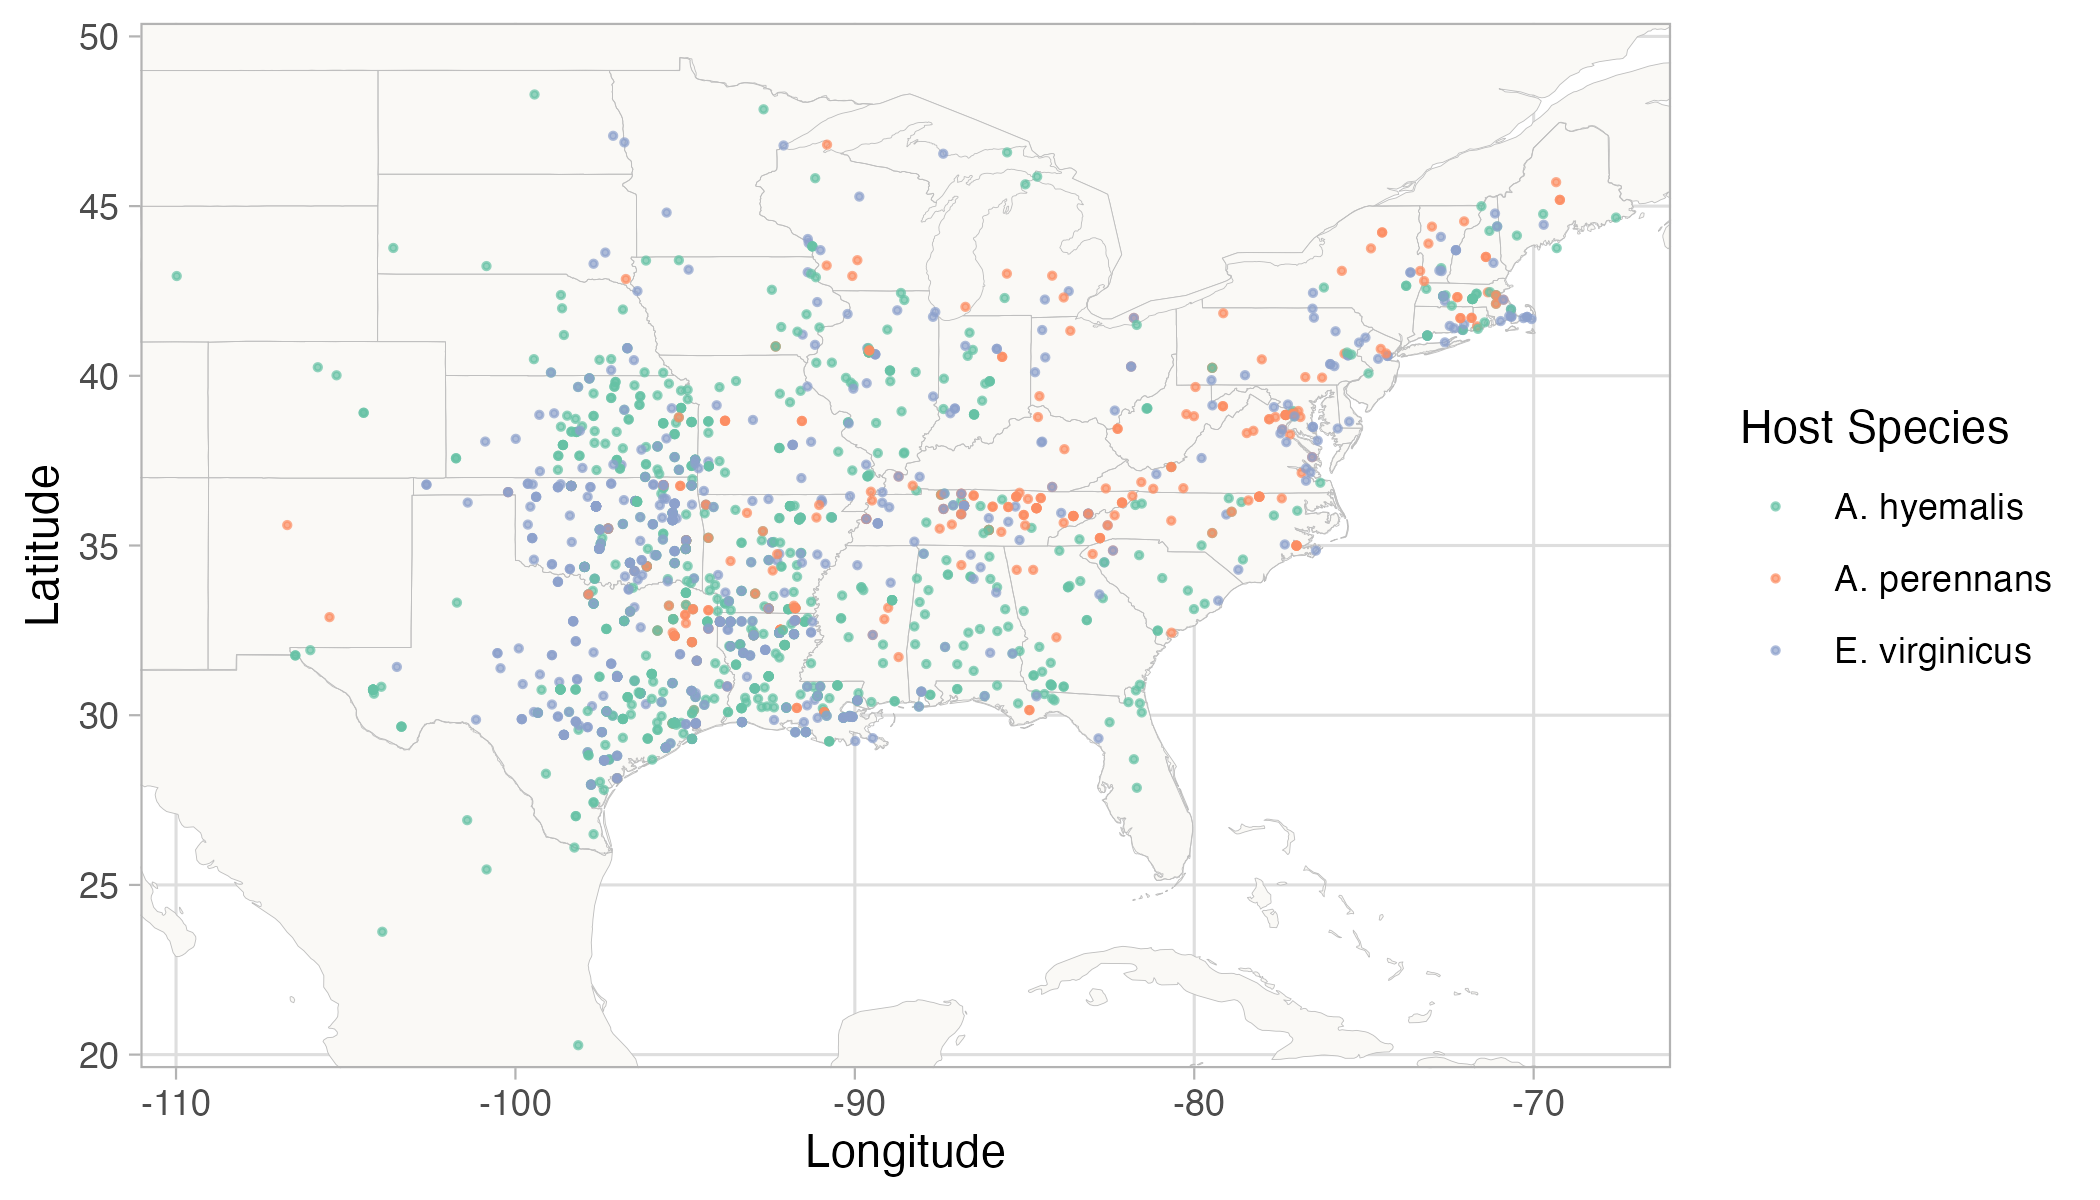
\includegraphics[width = \linewidth]{collections_map.png}
	\caption{\textbf{Collection locations of herbarium specimens of three grass host species across eastern North America that were sampled for \emph{Epichloë} endophyte presence or absence}.}
	\label{fig:map}
\end{figure}


\subsection*{Modeling spatial and temporal changes in endophyte prevalence}
We assessed spatial and temporal changes in endophyte prevalence across each host distribution, first quantifying the ``global'' trends, aggregating across space, and then examining spatial heterogeneity in the direction and magnitude of endophyte change (hotspots and coldspots) across the spatial extent of each host's distribution.
\tom{To appropriately account for the spatial non-independence of geo-referenced occurrences we used an approximate Bayesian method, Integrated Nested Laplace Approximation (INLA), to construct spatio-temporal models of endophyte prevalence.
INLA provides a computationally more efficient method of ascertaining parameter posterior distributions for certain models that can be formulated as latent Gausssian Models \cite{rue2009approximate}. 
Many common statistical models, including structured and unstructured mixed-effects models, can be represented as latent Gaussian Models. 
Fitting models with structured spatial effects is possible with MCMC sampling but can require long computation times, making INLA an effective alternative, which has been used to model spatial patterns in flowering phenology \cite{willems2022forest}, the abundance of bird species \cite{meehan2019spatial} and butterflies cite{crossley2022opposing}, the distribution of temperate trees \cite{engel2022spatial} as well as the population dynamics of endangered amphibians \cite{knapp2016large} and other ecological processes \cite{beguin2012hierarchical}.}{I think we need another sentence or two in this paragraph that provides an intuitive explanation for why INLA is the right approach for our analysis, written specifically for people who don't know what INLA is and don't want to know. I know the model includes a spatial decay term that controls spatial autocorrelation, a feature that I think is worth highlighting.}

First, to quantify global trends in endophyte prevalence, we modeled endophyte presence/absences of the $i^{th}$ specimen ($P_i$) as a Bernoulli response variable with expected probability of endophyte occurrence $\hat{P_i}$. 
We modeled $\hat{P_i}$ as a linear function of collection year and accounting for random effects associated with location ($l[i]$, a unique latitude-longitude combination), collector identity ($c[i]$), and scorer identity ($s[i]$) of the $i^{th}$ specimen.
\begin{subequations}
	\label{eq:trends}
	\begin{align}
		logit(\hat{P}_{i}) = \alpha_{l[i]} + \beta*year_i + \chi_{c[i]} + \omega_{s[i]} 
	\end{align}
\end{subequations}
Spatially-indexed random intercepts $\alpha_{l[i]}$ account for potential spatial autocorrelation between data points, and year slope $\beta$ describes the overall temporal trend in endophyte prevalence. 
We accounted for potential biases introduced during the process of collecting specimens as well as in scoring ability by including random effects specific to each collector $\chi$ and scorer $\omega$.
Previous work suggests that behavior of historical botanists and uneven sampling may introduce biases into ecological inferences made from historic collections \cite{kozlov2020biases}. 
Prolific collectors who contribute thousands of specimens may be more or less likely to collect certain species, or specimens with certain traits \cite{daru2018widespread}. 
Similarly, the process of scoring seeds for hyphae involved many student researchers who, even with standardized training, may vary in their likelihood of positively identifying \emph{Epichloë} hyphae. 
By including a random effect for collectors and for scorers, we accounted for variance across individual researchers that may bias our predictions of changes in endophyte prevalence.
\tom{Models for each host species were fit separately.}{It would be great to pull all species into one model and have them share variance terms for the random effects. I suspect such a model would give better and more stable estimates.}
\tom{}{I updated the notation in ways that make more sense to me, but you should check that this is true to the actual model (I think it is). Also, a more complete presentation of this model would show the variance terms for $\alpha$, $\chi$, and $\omega$. I presume the latter two are Gaussian but I don't know how to represent the distribution of $\alpha$.}


Second, to quantify how temporal trends may vary spatially, we repeated the modelling above, but incorporated a spatially-varying coefficient for collection year:
\begin{subequations}
	\label{eq:trends}
	\begin{align}
		logit(\hat{P}_{i}) = \alpha_{l[i]} + \beta_{l[i]}*year_i + \chi_{c[i]} + \omega_{s[i]} 
	\end{align}
\end{subequations}
The spatially-varying year slope $\beta_{l}$ allowed us to flexibly estimate variation in the temporal trajectory of endophyte change at locations across the study region.

\tom{For both models, spatially-structured random intercepts ($\alpha_{l}$) and slopes ($\beta_{l}$) were constructed using stochastic partial differential equations (SPDE) that depend on a covariance matrix according to the proximity of each collection location \citep{lindgren2011explicit,bakka2018spatial}. 
The covariance matrix was approximated using a Mat\'{e}rn covariance function, with each data point assigned a location according to the nodes of a mesh of non-overlapping triangles across our study area (Fig A2).}{This paragraph would be a place to describe the variance terms for the other random effects.}

We performed model fitting using the inlabru R package \citep{}, \tom{with vague priors}{I thought you needed informative priors on the spatial decay parameters}, and compared models with different sizes of mesh, \tom{which had little effect on the resulting model estimates}{That'sa good but you still need to state what mesh size you used and what that means, biologically.}.
Each \tom{mesh}{You have not defined what you mean by ``mesh''.} was bounded by the predicted host distribution, described below.
Posterior modes were \tom{stable}{Assessed how?} indicating that numeric convergence was successful.
We assessed model fit with graphical posterior predictive checks (Fig. A3).
\tom{The model performed adequately at classifying the historical data, comparing the accuracy of predictions from the model with observed data (avg. AUC = 0.77; Fig. A4). }{Maybe move this to validation section, and then have both in-sample and out-of-sample approaches.}

\subsection*{Modeling distributions of host species}
We modeled  epicloe host species distribution to predict their occurrences in space and time as continuous and binary maps of potential presences. 
These maps were used as a backbone to predict endophyte prevalence on epicloe host species. 
The species distribution models were built following the ODMAP (overview, data, model, assessment, prediction) protocol \citep{crossley2022opposing}. 
We used the observed presence of the host species collected from GBIF from 1990 to 2020. These occurrences were corrected for spatial autocorrelation due to sampling bias by thinning the occurrences to the spatial scale of the climatic variables. The climatic variables were temperature of the spring, precipitation of the spring  and precipitation of the summer. We preferred these variables because they were not correlated (Variance Inflation Factor \> 0.7) and also allowed the model to account for the influence of seasonal climate variation on species presence.
The occurrence data was split into 75\% for model training and 25\% for model testing. We fitted the model using maximum entropy (MaxEnt) using the maxent function in the package dismo \citep{hijmans2017package}. 
MaxEnt was preferred because it does not generate response curves that may cause unpredictable behavior when applied to new climates \citep{hijmans2006ability}.
 We used 10000 pseudo-absences as background points. 
 To convert the continuous predicted probabilities into binary presence - absence maps, we used the  training sensitivity (true positive rate) and specificity threshold (true negative rate) \citep{liu2005selecting}. 
The performances of the model were evaluated using the AUC \citep{jimenez2012insights}. 


\subsection*{Validating the model with an out-of-sample test}
We evaluated the predictive ability of the model using contemporary endophyte surveys as out-of-sample test data, \tom{an important but rarely used strategy in ecological studies \cite{tredennick2021practical}.}{This is the type of thing to emphasize in the intro? Are there any other collections-based papers that have done anything like this?? None to my knowledge.} 
We used data from contemporary surveys of endophyte prevalence  in \emph{A. hyemalis} and \emph{E. virginicus} in Texas and the southern US. 
Surveys of \emph{E. virginicus} were conducted in 2013 as described in \citet{sneck2017variation}, and \tom{surveys of \emph{A. hyemalis} took place between 2015 and 2020}{We have added more recent AGHY survey data. I am not sure if you have access to this but you should definitely use it. Karl or I can point you to the right file.}.
Population surveys of \emph{A. hyemalis} were initially designed to cover longitudinal variation in endophyte prevalence towards its range edge, while surveys of \emph{E. virginicus} were designed to cover latitudinal variation along its range edge. 
In total, we visited 43 populations of \emph{A. hyemalis} and 20 populations of \emph{E. virginicus} across the south-central US, with emphasis on Texas and neighboring states (Fig \tom{A4}{This is now A6. Good reminder to use the ref function.}).
During surveys, we collected seeds from up to 30 individuals per location  (average number of plants sampled: 22.9).
We quantified the endophyte status of each individual with staining microscopy as described for the herbarium surveys (with 5-10 seeds scored per individual), and calculated the prevalence of endophytes within the population (proportion of symbiotic plants divided by the number of sampled plants).
For each population, we compared the observed fraction of endophyte-symbiotic hosts to the predicted probability of endophyte occurrence $\hat{P}$ derived from the model based on location and year, with collector and scorer random effects fixed at zero. 
\tom{The contemporary survey period (2013-2020) is at the most recent edge of the time period encompassed by the historical observations used for model fitting.
We compared the model's prediction for these locations to the observed population prevalence.}{It is not clear if you are testing model 1 (``global trend'') or model 2 (``spatially varying trends'').}

\subsection*{Assessing the role of climate drivers}
We assessed how the magnitude of climate change may have driven changes in endophyte prevalence by assessing correlations between changes in climate and changes in endophyte prevalence predicted from our spatial model at evenly spaced pixels across the study area.
We first downloaded monthly temperature and precipitation rasters from the PRISM climate group \citep{daly2013prism} covering the time period between 1895 and 2020 using the 'prism' R package \citep{Rprism2015}. 
Prism provides reconstructions of historic climate variables across the United States by spatially-interpolating weather station data \citep{diLuzio2008constructing}. 
We calculated 30-year climate normals for annual and seasonal mean temperature and cumulative precipitation for the recent (1990 to 2020) and historic (1895 to 1925) periods.
We used three four-month seasons within the year (Spring: January, February, March, April; Summer: May; June, July, August; Autumn: September, October, November, December). 
This division of seasons allowed us to quantify differences in climate associated with the two ``cool'' seasons, when we expect our focal species to be most biologically active (\emph{A. hyemalis} flowering phenology: Spring; \emph{E. virginicus}: Spring and Summer; \emph{A. perennans}: Fall). 
In addition to mean climate conditions, environmental variability itself can influence population dynamics \cite{tuljapurkar_population_1982} and changes in variability are a key prediction of climate change models \cite{stocker2013technical, ipcc_2021}.
Therefore we calculated the coefficient of variation (CV) during each period for each annual and seasonal climate driver as the interannual standard deviation divided by the mean across each 30-year period.
We then took the difference between recent and historic periods for the mean and CV for each climate driver \tom{(Fig. A5)}{This is Figure A7 -- Can you make the color scale on these diverging at zero?}.
Because initial analyses indicated a high degree of collinearity between seasonal and annual changes in temperature, we used annual temperature only, along with annual and seasonal precipitation, in the subsequent analysis.
All together, this left us with measurements of change in 10 potential climate drivers: the mean and coefficient of variation of annual temperature, as well as the mean and coefficient of variation of cumulative annual precipitation, cumulative spring precipitation, cumulative summer precipitation, and cumulative autumn precipitation \jacob{(Fig A8-A9)}{ The species names are not clear  on Fig A9. I suggest increase the font siize }.

To evaluate whether areas that have experienced the greatest changes in endophyte prevalence (hotspots of endophyte change) are associated with high degrees of change in climate (hotspots of climate change), \tom{we modeled spatially varying slopes of endophyte change through time ($\beta_{l}$) as a linear function of environmental covariates, with a Gaussian error distribution. }{I think we need to account for uncertainty in the slopes. They are outputs of a (quasi) Bayesian model so we should be able to propagate all the uncertainty in the posterior disgtribution.}
Calculating correlations from many pixels across the study region risks articially inflating confidence in our results due to large sample sizes, and \tom{so we repeated this calculation using only a random subsample of 100 pixels across the study region}{100 seems like a low number to me. What if we did this for all of the herbarium collection locations?}.
\tom{}{Are the methods above repeated for each species separately?}
\tom{}{I cut the notation for the Gaussian model for now because it is a pretty simple model and the notation may be overkill, plus because I changed your tau's to beta's there were betas on both sides of the tilde, which was confusing/annoying. Happy have the notation back if you prefer it. I am also a little confused because the appendix has spearman correlations but there are no methods here for where those come from.}


%We evaluated how predicted changes in endophyte prevalence ($\Delta{P}$) correlated with %changes in seasonal climate at a grid of points across the study area using linear regression.

%\begin{subequations}
	%\label{eq:climate}
	%\begin{align}
		%\Delta{P} \sim Normal(\mu, \sigma)\\
		%\mu = \beta_{0} + \alpha_{1}*\Delta{Precip_{spring}} + %\alpha_{2}*\Delta{Precip_{summer}} + \alpha_{3}*\Delta{Precip_{autumn} }+ \\ %\alpha_{4}*\Delta{Temp_{spring}} + \alpha_{5}*\Delta{Temp_{summer}}  + %\alpha_{6}*\Delta{Temp_{autumn}} 
%	\end{align}
%\end{subequations}

 %The change in prevalence is determined by an intercept $\beta_{0}$ slopes specific to the seasonal %changes in preciptation ($\alpha_{1}$, $\alpha_{2}$, and $\alpha_{3}$) and in mean %temperature ($\alpha_{4}$, $\alpha_{5}$, and $\alpha_{6}$).
 %We fit models for each host species separately with rINLA using default vague priors.
		
\section*{Results}
\subsection*{How has endophyte prevalence changed over time?}
We found that endophyte prevalence increased within the examined specimens over the last two centuries for all three host species (Fig. 4). 
On average, \emph{A. hyemalis} and \emph{E. virginicus} both increased from ~30 \% to over 70\% prevalence across the study region, and \emph{A. perennans} increased from ~ 15\% to over 70\% prevalence.
\josh{Our model indicates a higher certainty that overall temporal trends are positive for \emph{A. hyemalis} and \emph{A. perennans} than for \emph{E. virginicus} (99\% probability of a positive overall year slope in \emph{A. hyemalis}, 89\% probability of a positive overall year slope in \emph{A. perennans}, and 58\% probability of a positive overall year slope in \emph{E. virginicus}) .}{These numbers are currently outdated. I am making some adjustments to models, and will update with final model}

\begin{figure}[H]
	\centering
	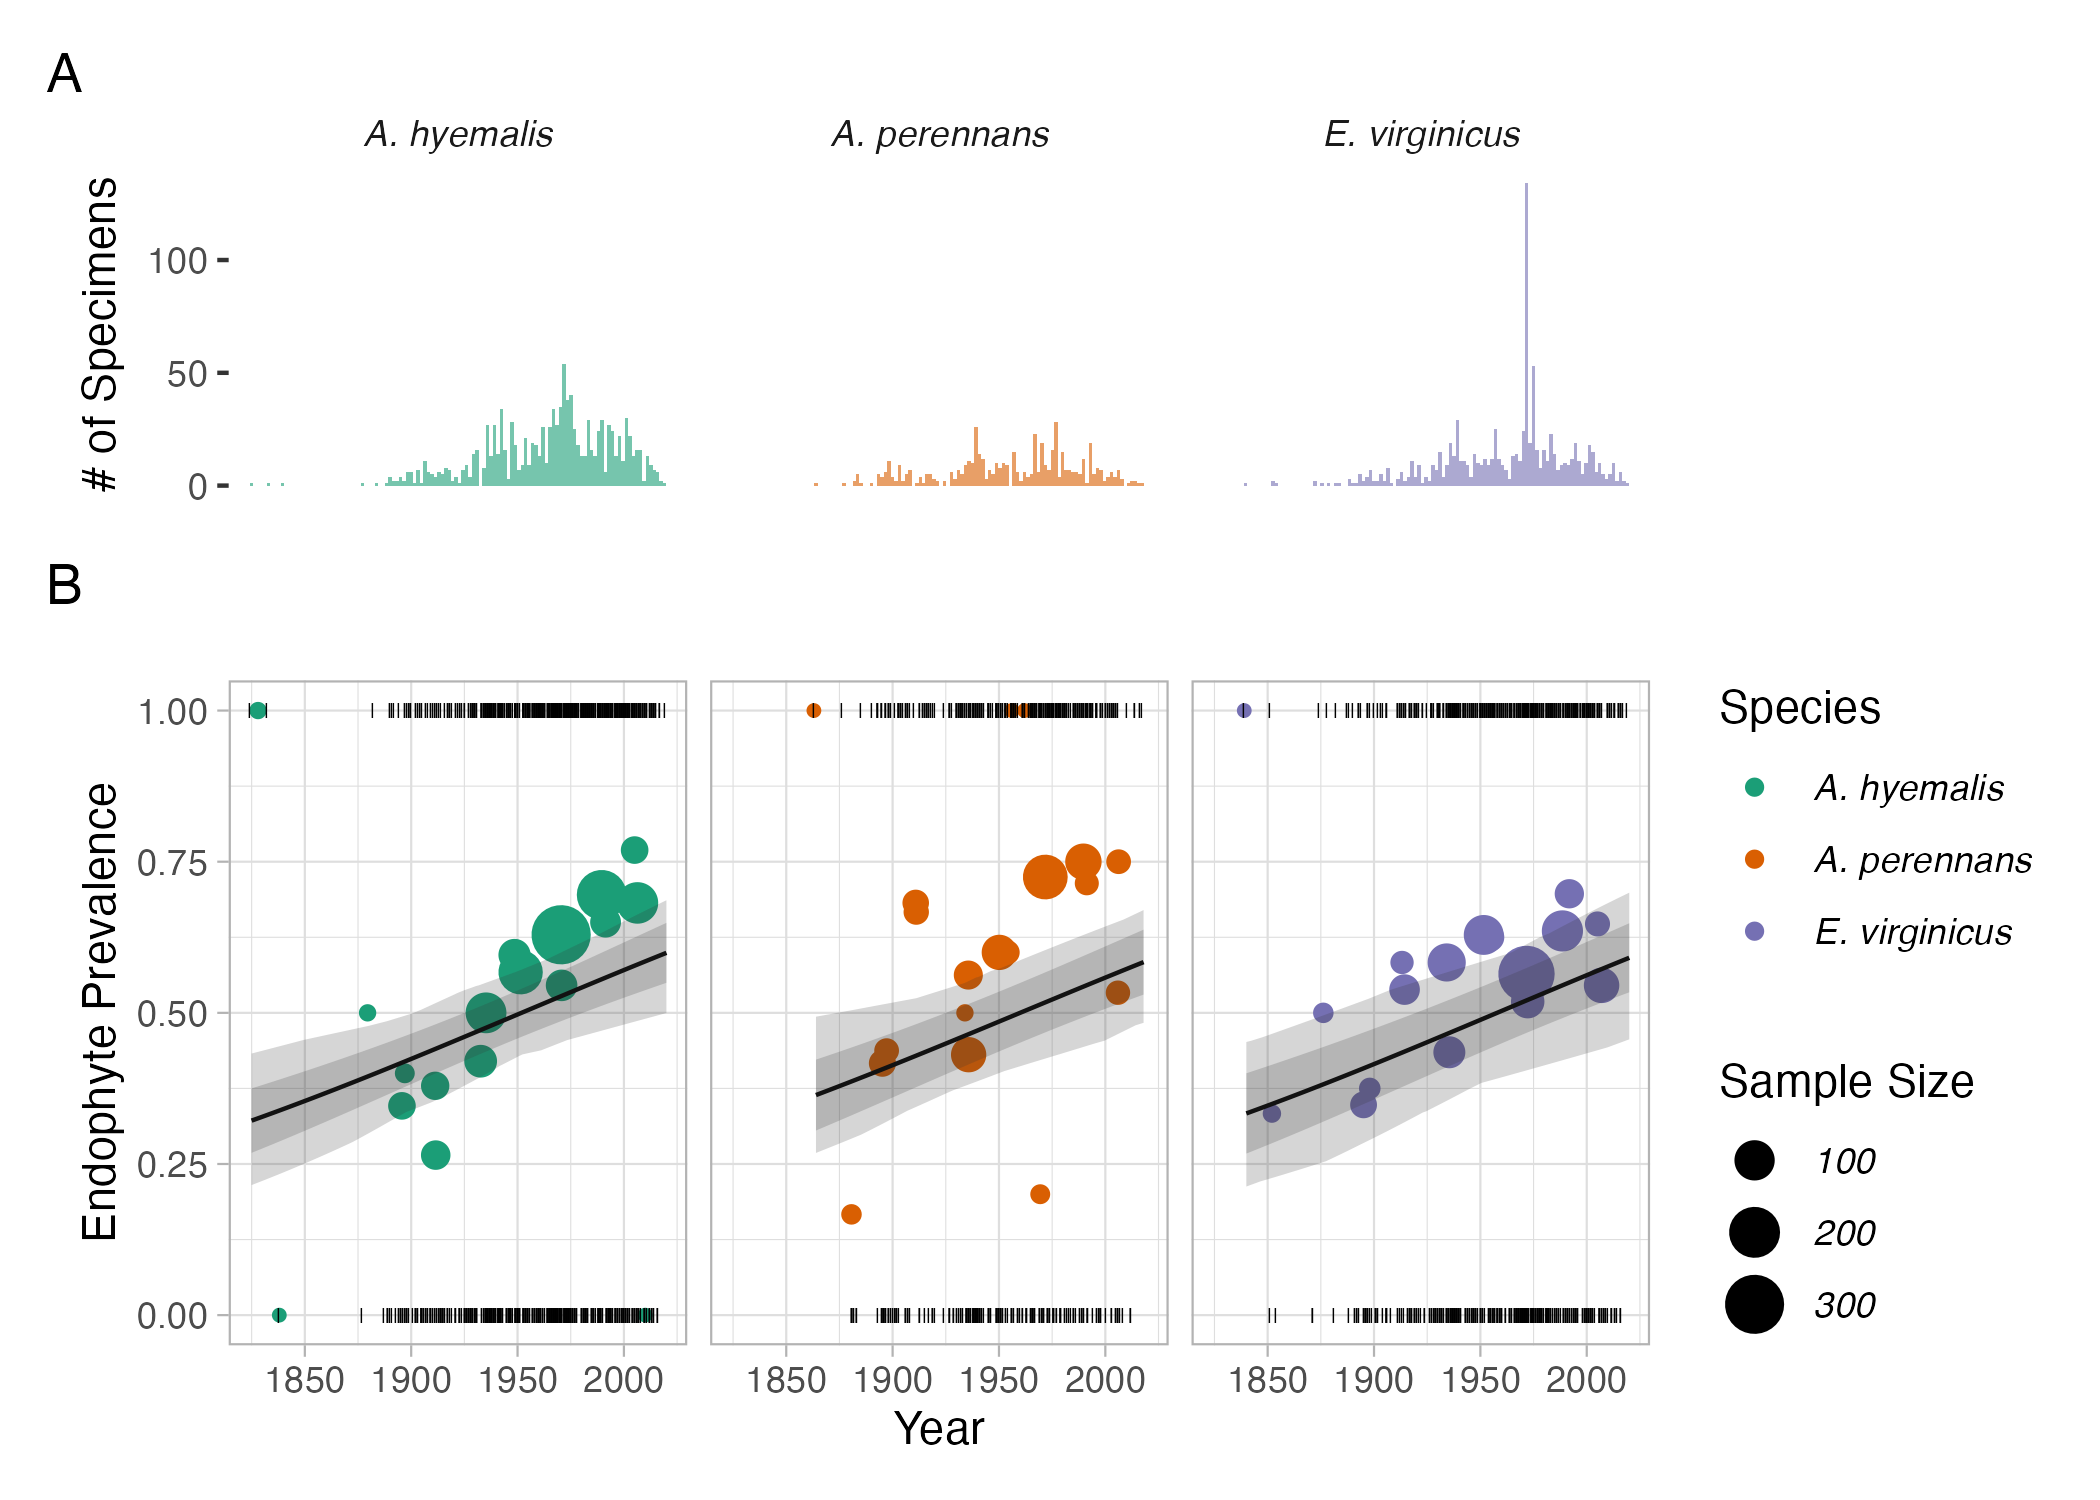
\includegraphics[width = \linewidth]{year_plot.png}
	\caption[Temporal trends in endophyte prevalence.]{Temporal trends in endophyte prevalence. (A) Histograms show the frequency of collection through time for each host species. (B) Colored points are binned means of the observed endophyte presence/absence data (black dashes). Colors represent each host species and point size is determined by the number of specimens. Lines show predicted mean endophyte prevalence over the study period along with the 50\%  and 95\% CI bands.}
	\label{fig:temporal}
\end{figure}




\subsection*{How spatially heterogenous are temporal trends in endophyte prevalence?}
Our model revealed hotspots of change in endophyte prevalence . 
While there was an overall increase in endophyte prevalence, these changes varied across the host species' ranges (Fig. 3).
In some regions, posterior estimates of our spatially varying temporal trends, $\tau$, indicate that \emph{A. hyemalis} and \emph{A. perennans} experienced increases in percent prevalence by as much as 4\% per year over the study period, while  \emph{E. virginicus} experienced increases up to around 1.5 \% per year. 
In other regions, there were negligible changes. Notably, the symbionts of \emph{E. virginicus} experienced only slight increases in prevalence, and were less spatially variable than the other two species. 
\josh{Regions that start with low endophyte prevalence, as in the southwestern portion of the range of \emph{A. hyemalis}(Fig. A1), also experienced negligible change, suggesting that this may be driven more by the absence of the endophyte.}{more discussion material, but putting it here for now.}
Predicted trends for \emph{A. perennans} show certain areas of both large increase and of large decrease, however this species, for which we have the fewest samples, has the largest uncertainty.
The posterior estimates of our spatially varying temporal trends, indicate relatively narrow certainty (\josh{need to compute}{}).

\begin{figure}[H]
	\label{fig:svc_time_map}
	\centering
	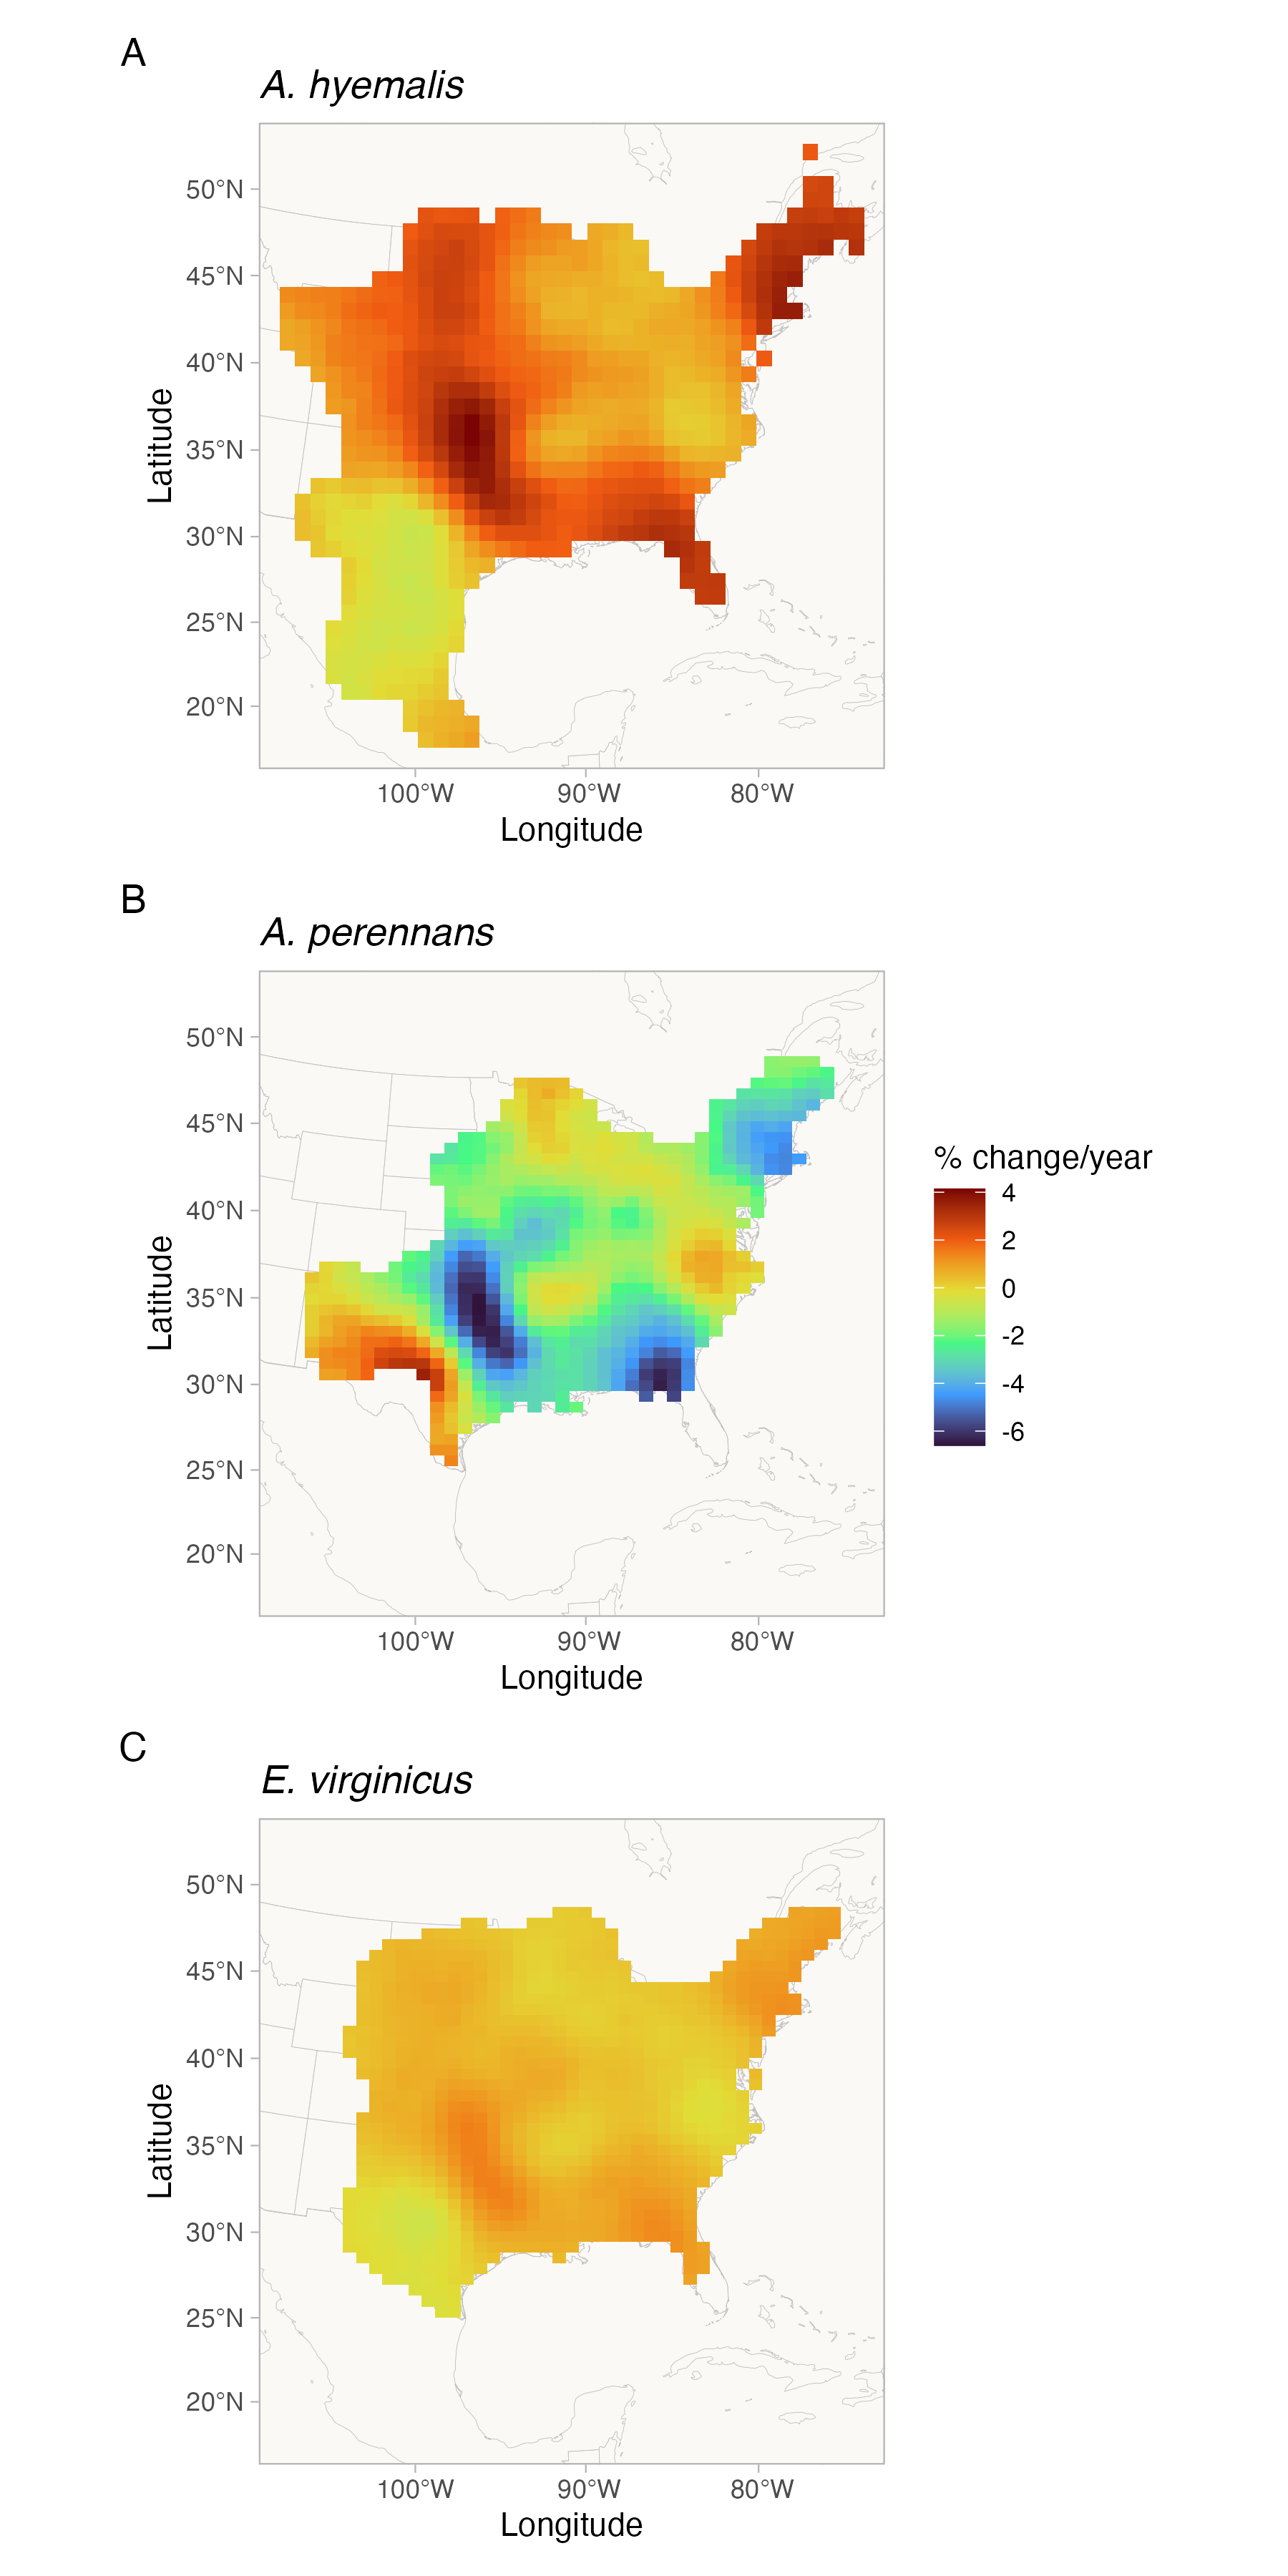
\includegraphics[width = .6\linewidth]{svc_time_map.png}
	\caption[Predicted posterior mean of spatially-varying slopes representing change in endophyte prevalence for each host species.]{Predicted posterior mean of spatially-varying slopes representing change in endophyte prevalence for each host species. Color indicates the relative change in predicted endophyte prevalence.}
\end{figure}









\subsection*{Assessing collector and scorer influences on predicted endophyte prevalence}
We quantified temporal and spatial trends in endophyte prevalence while accounting for potential biases introduced by collectors and by individuals who quantified endophyte presence/absence with the use of random effects. 
We found no evidence that collector biases influenced our results. 
Collector random effects were consistently small; Fig 4A, and models fit with and without this random effect provide qualitatively similar results.
The identity of individual scorers did contribute to observed patterns in endophyte prevalence.
For example, 3 of the 16 scorers were more likely than average to assign positive endophyte status, as indicated by 95\% credible intervals that do not overlap 0) (Fig 4B). 
However, this may have been driver by differences in scorers biases during the seed scoring process, or by unintended spatial clustering of the specimens scored by each scorer. 
Interpreting our models with the inclusion of the scorer effect thus provides conservative estimates of the absolute magnitude of changes in endophyte prevalence.

\begin{figure}[H]
	\label{fig:random_fx}
	\centering
	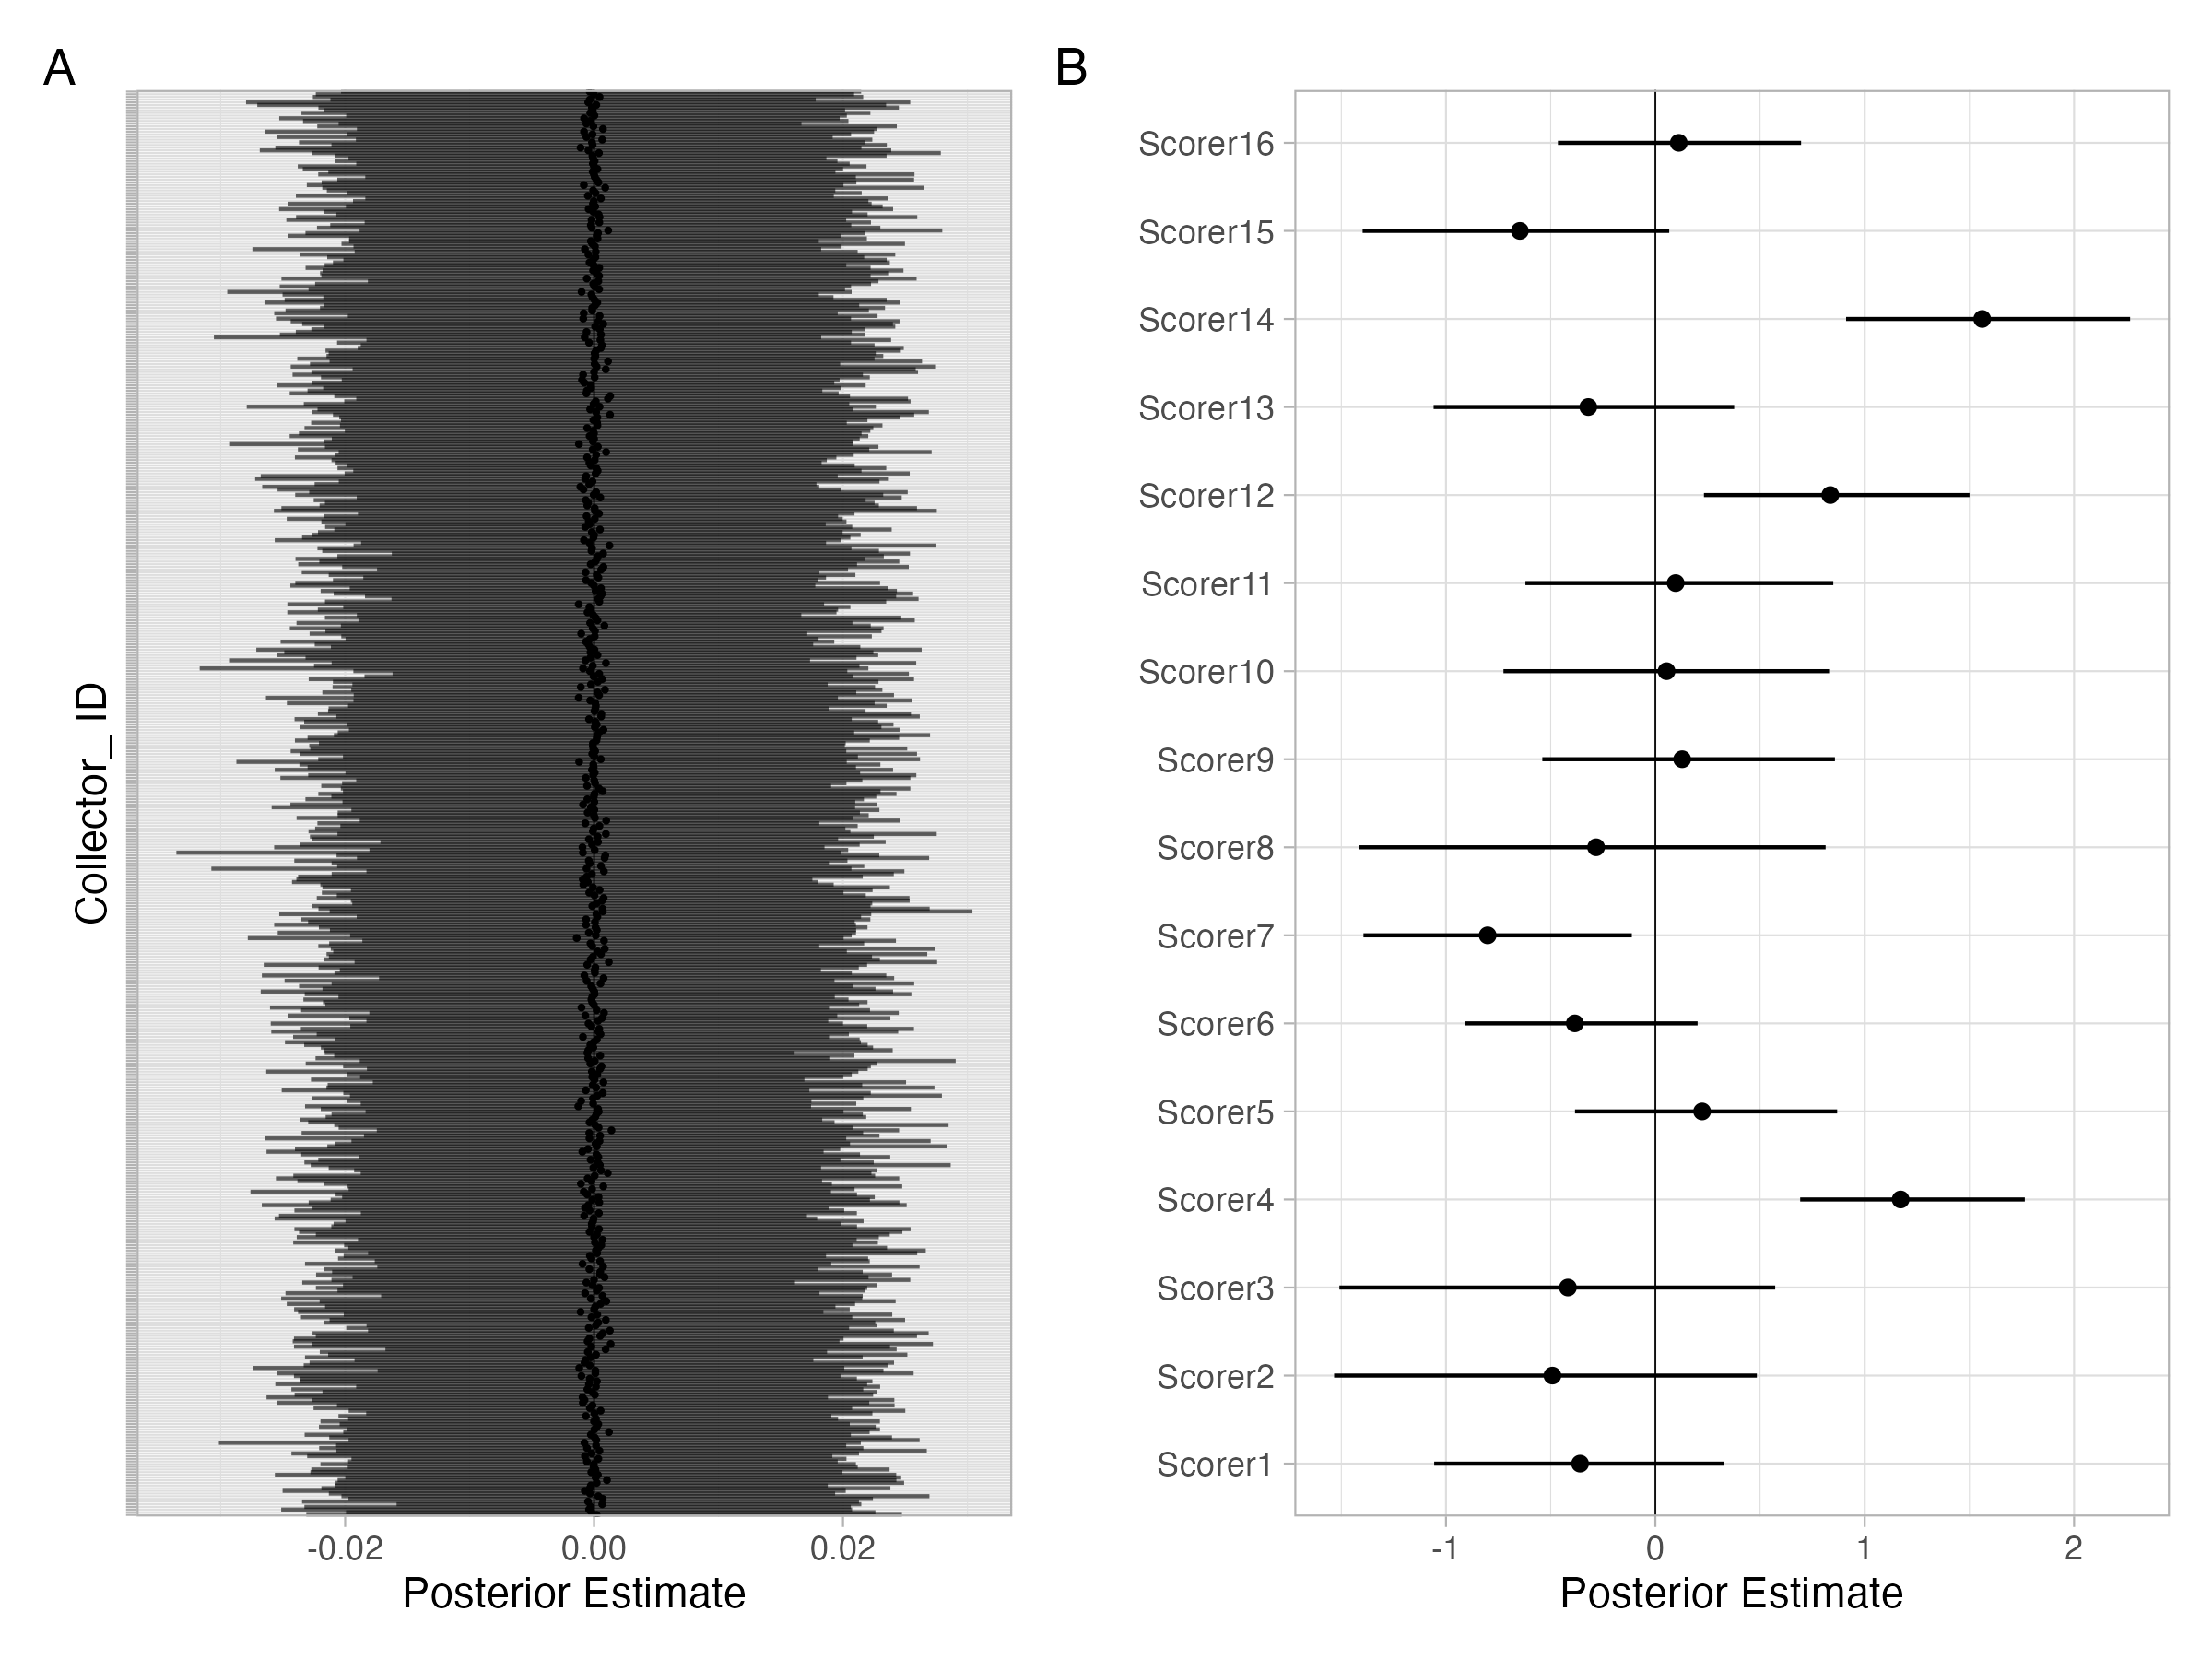
\includegraphics[width = .8\linewidth]{random_fx_plot.png}
	\caption{\textbf{Posterior estimates of (A) collector and (B) scorer random effects.} Points show the posterior mean along with 95\% CI for random effects estimate from 532 collectors and 16 scorers.}
\end{figure}


%\subsubsection*{How does endophyte prevalence vary across space?}
%Across space, there were clear trends in endophyte prevalence which varied between species (Fig. 5).
%We mapped predictions of endophyte prevalence across the area encompassing the sampled herbarium specimens for each species, and area smaller than the full geographic distribution of each species in nature.
%\emph{Elymus virginicus} had higher prevalence towards the northern portions of the collection range. 
%In contrast, \emph{Agrostis hyemalis} had highest prevalence towards the center of its collection range with regions of low prevalence towards the northeast and towards its western range edge.
%\emph{Agrostis perennans} had  highest prevalence towards the westernmost portion of its collection range.
%There is considerable uncertainty in the spatial pattern of endophyte prevalence (See Fig. A10 for projections of the 95\% credible interval), however these broad spatial patterns are consistent across the low and high end of model predictions. 

\begin{figure}[H]
	\label{fig:svc_space_map}
	\centering
	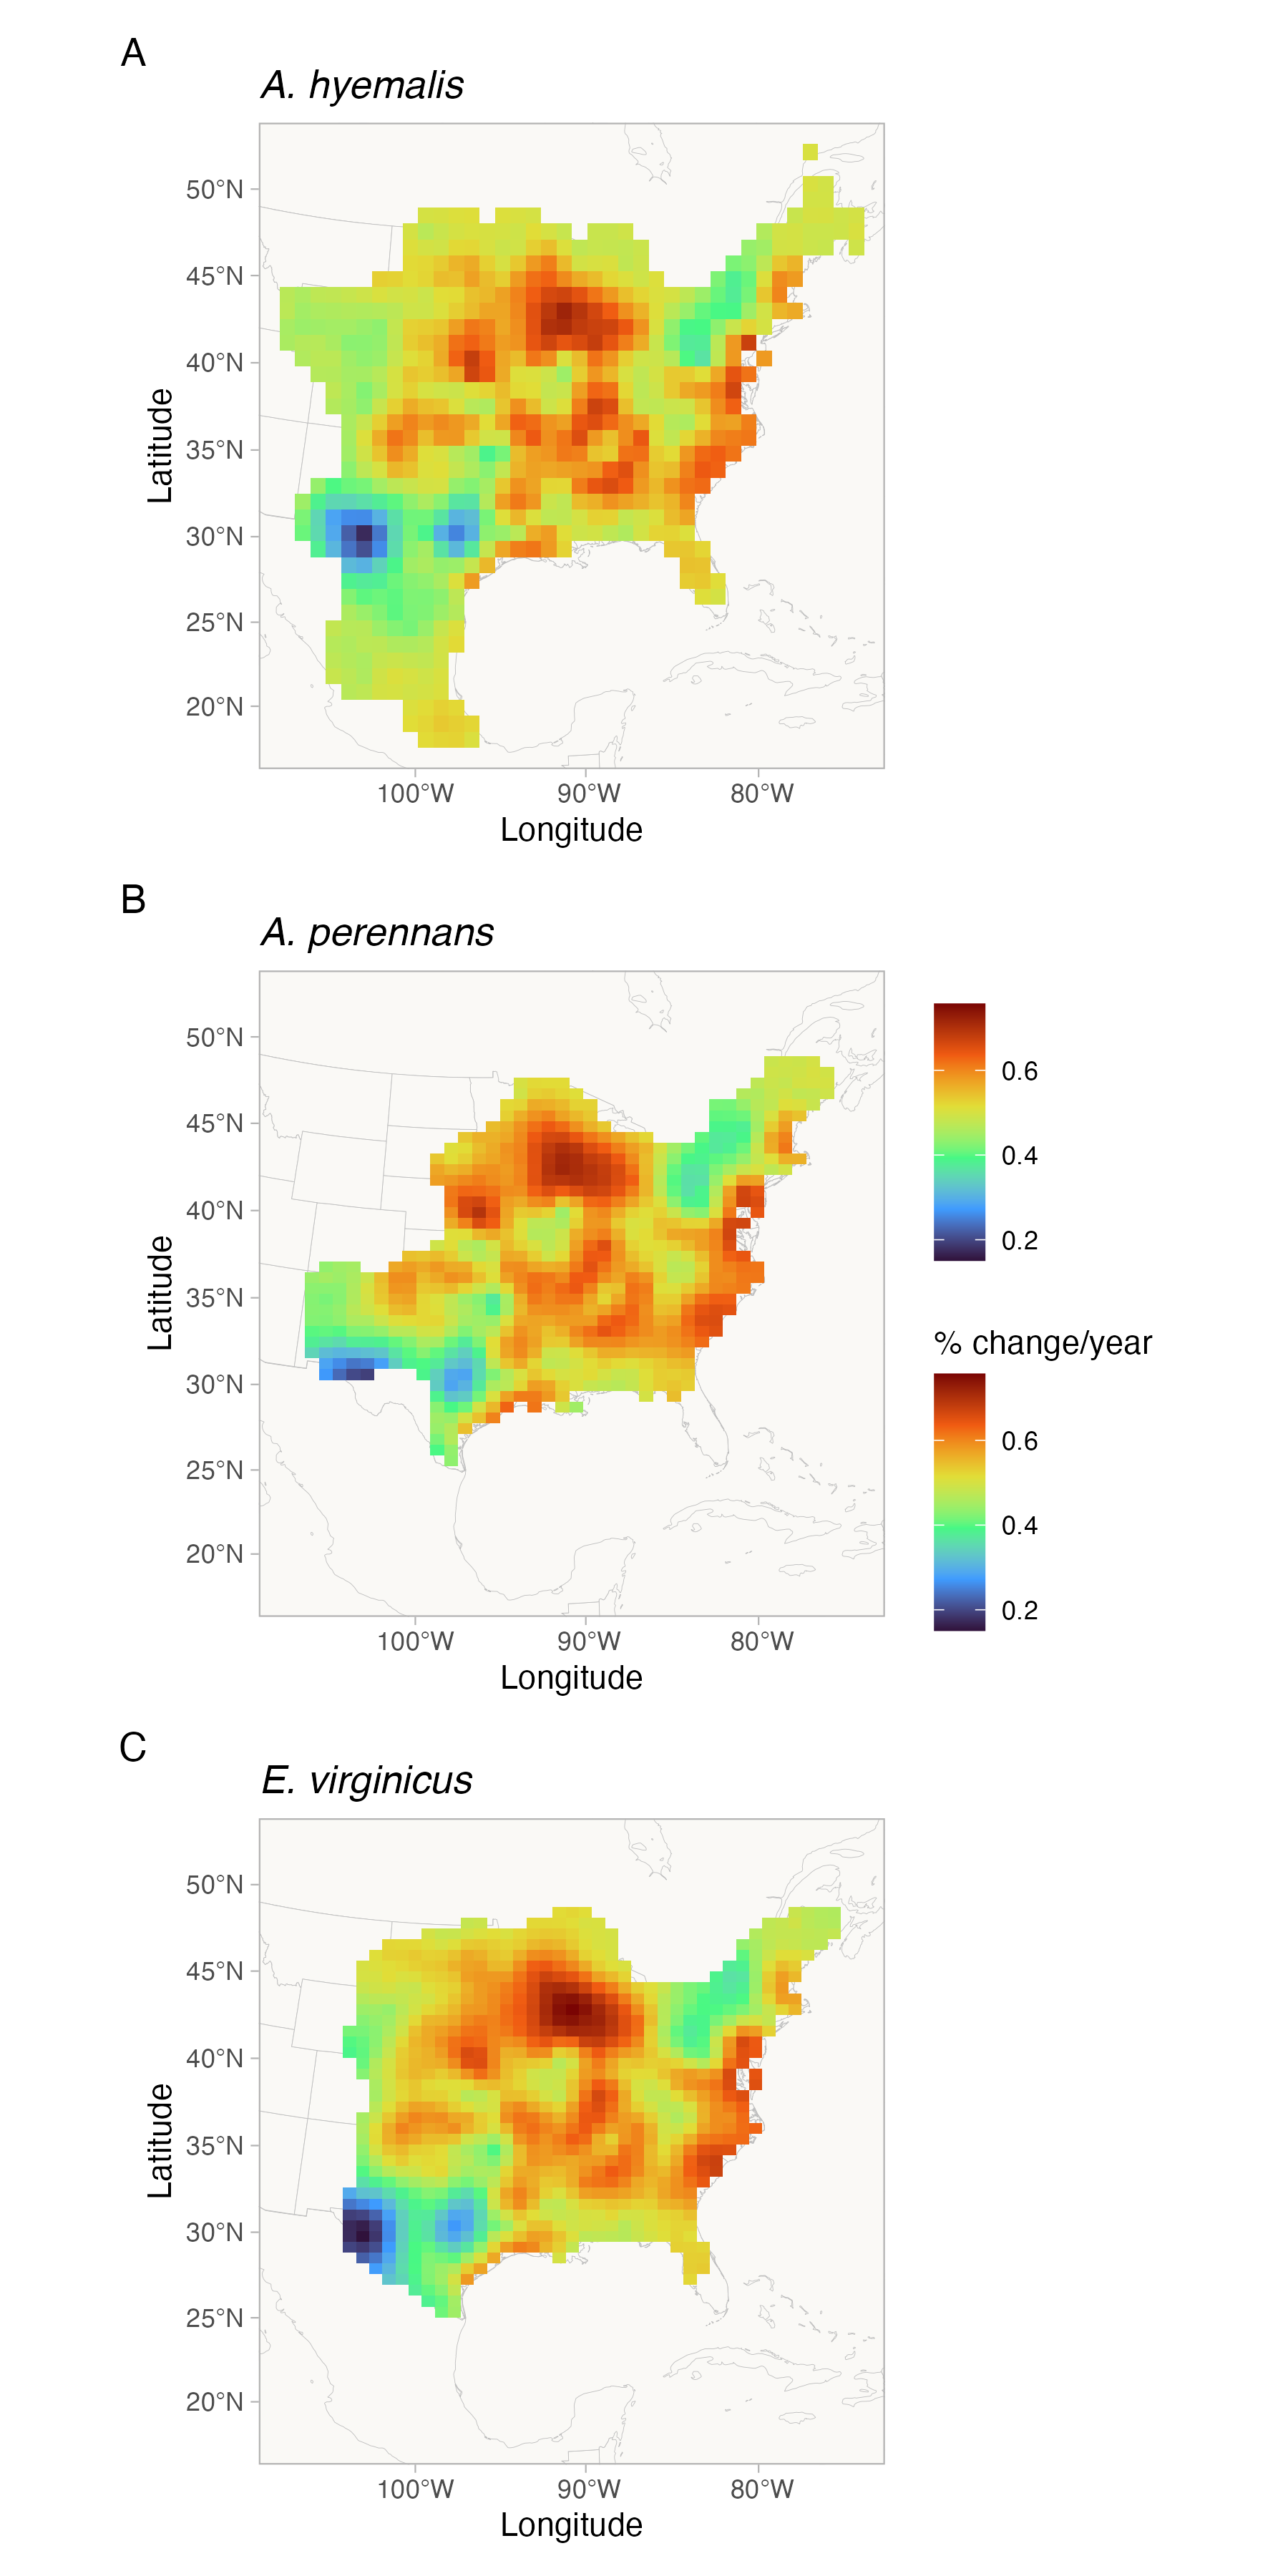
\includegraphics[width = .6\linewidth]{svc_space_map.png}
	\caption{\textbf{Mean predicted endophyte prevalence for each host species (columns) in 1925 (top row) and 2020 (bottom row)}. Color indicates mean predicted rate of endophyte prevalence across the predicted distribution of each species.}
\end{figure}





\subsection*{What is the relationship between variation in temporal trends in endophyte prevalence and changes in climate drivers?}

We found that trends in endophyte prevalence were strongly associated with seasonal climate change drivers (Fig. 6).
For the majority of the study region, the climate has become wetter and cooler over the last century (Fig. A7-A8), a consequence of regional variation in global climate change \cite{ipcc_2021}. 
Within the study region, spatially heterogeneous environmental changes were predictive of changes in endophyte prevalence. 
For example, strong increases in prevalence within \emph{E. virginicus} were most associated with declines in Summer precipitation  (a negative correlation in Fig. 7) as well as with increases in the year-to-year variability of annual temperature (a positive correlation in Fig. 7). 
Changes were also associated with reductions in average annual temperatures, and increases in year-to-year temperature variability.
\emph{A. perennans} endophyte prevalence increased most strongly in regions that experienced reduced spring precipitation and reduced variability in annual temperature.
Although these correlations were weaker, changes in \emph{A. perennans} endophyte prevalence were also associated with increased in increases in annual precipitation and increasing autumn precipitation. 
For \emph{A. hyemalis}, endophyte prevalence increased most strongly in regions that experienced reductions in autumn precipitation variability. 
Correlations using only a subsampling of pixels were qualitatively similar to these results (Fig. A11), suggesting that the patterns we find are not spurious associations.

%These associations are in line with expectations that endophyte symbiosis provides drought tolerance to their hosts, particularly during \emph{E. virginicus}'s \tom{summer growing season}{It is a stretch to say that this species has a summer growing season.}. 
%For \emph{A. perennans}, which flowers in the late Summer and Autumn, increases in autumn precipitation along with increases in variability in annual precipitation, were strongly assocated with increasing endophyte prevalence.  
%While this result is contrary to the expectation that endophyte provide drought tolerance, this species typically is associated with wetter microhabitats, and it also \tom{suggests a role for endophytes to play in buffering the negative consequences of demographic variability \citep{lewontin_population_1969}}{I would save for discussion}.  
%For \emph{A. hyemalis}, which flowers in the Spring, changes in endophyte prevalence were more weakly associated with seasonal changes in climate drivers than for the other two species.
%It was, however, the only species' for which greater increases in endophyte prevalence were associated with regions that experienced increases in average annual temperatures.\tom{}{Is this a significant association, however you want to define that? Or could this result have occurred by chance?}
\josh{}{Only have plotted results for AGHY right now.}
\begin{figure}[H]
	\centering
	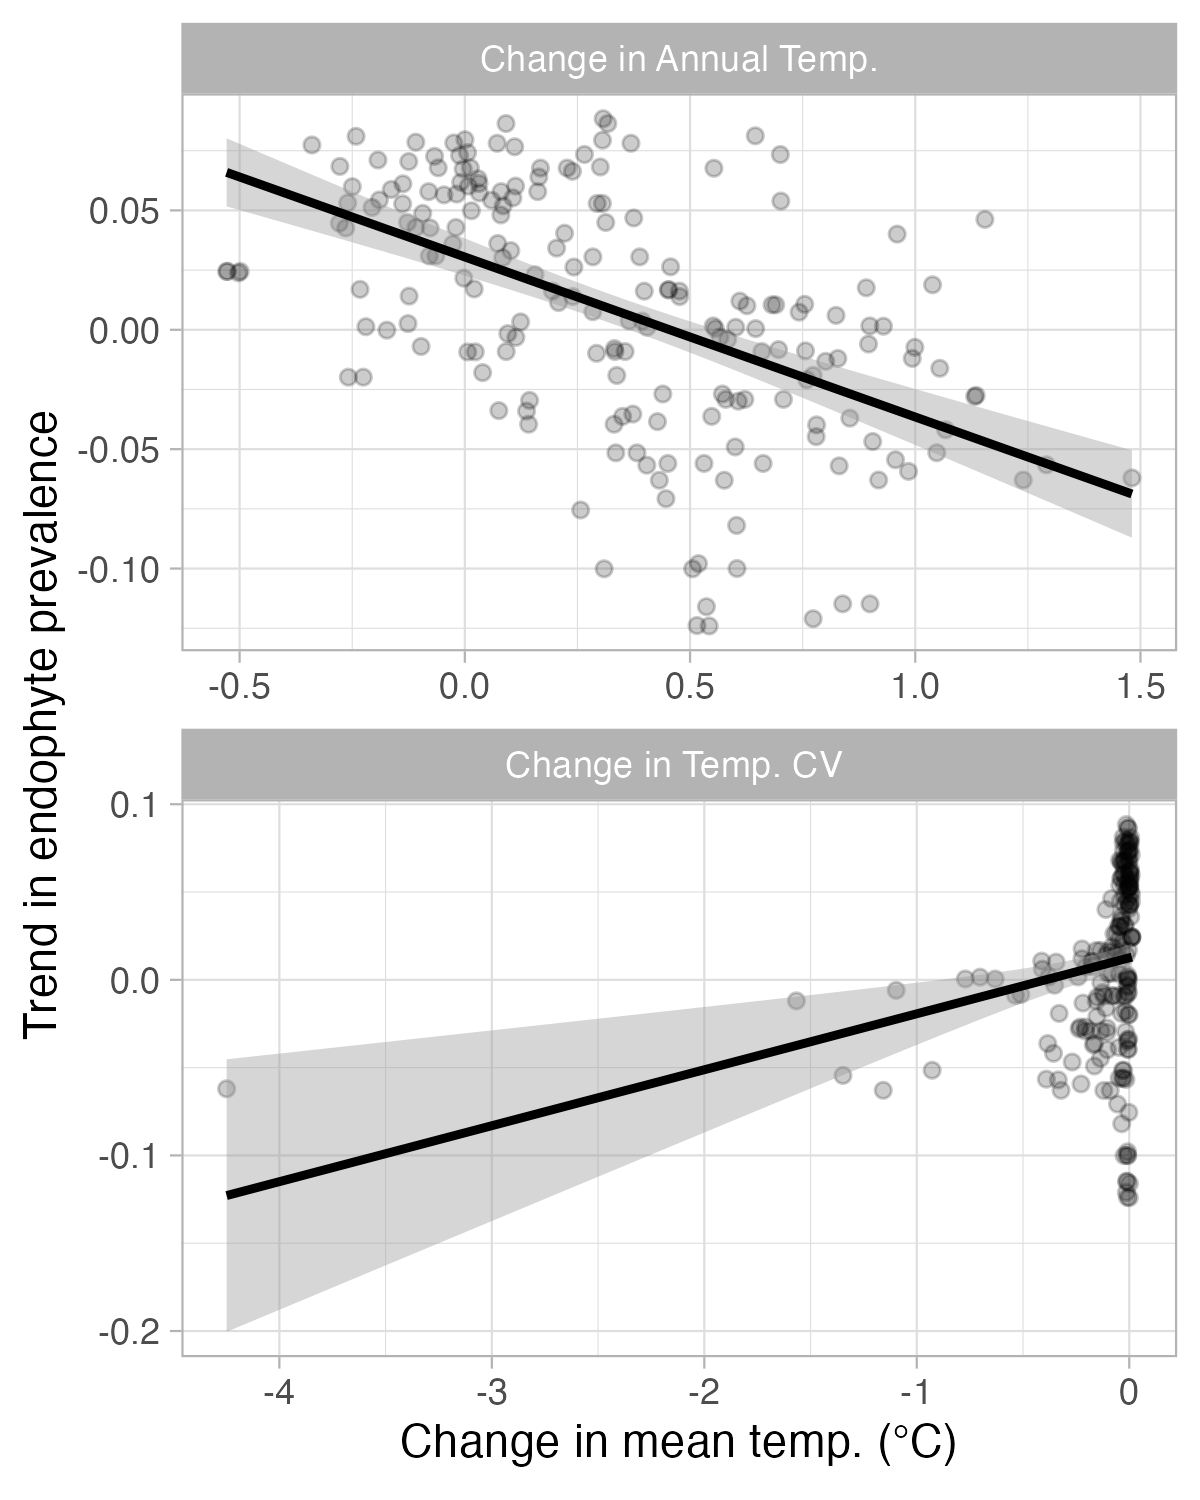
\includegraphics[width = .7\linewidth]{tmean_regression_plot_ESA.png}
	\caption{\textbf{Correlations between changes in climate drivers and changes in endophyte prevalence.} Color denotes the Spearman correlation coefficient between the relative rate of change in endophyte prevalence and the change in annual mean temperature ($^oC$) and total annual and seasonal precipitation (mm), as well as the change in the coefficient of variation of each climate driver. Positive correlation coefficients indicate that greater increases in a climate driver were associated with larger increases in endophyte prevalence, while negative values indicate that . Asteriks denote correlation coefficients $> .3$ or $< -.3$.}
\end{figure}

\begin{figure}[H]
	\centering
	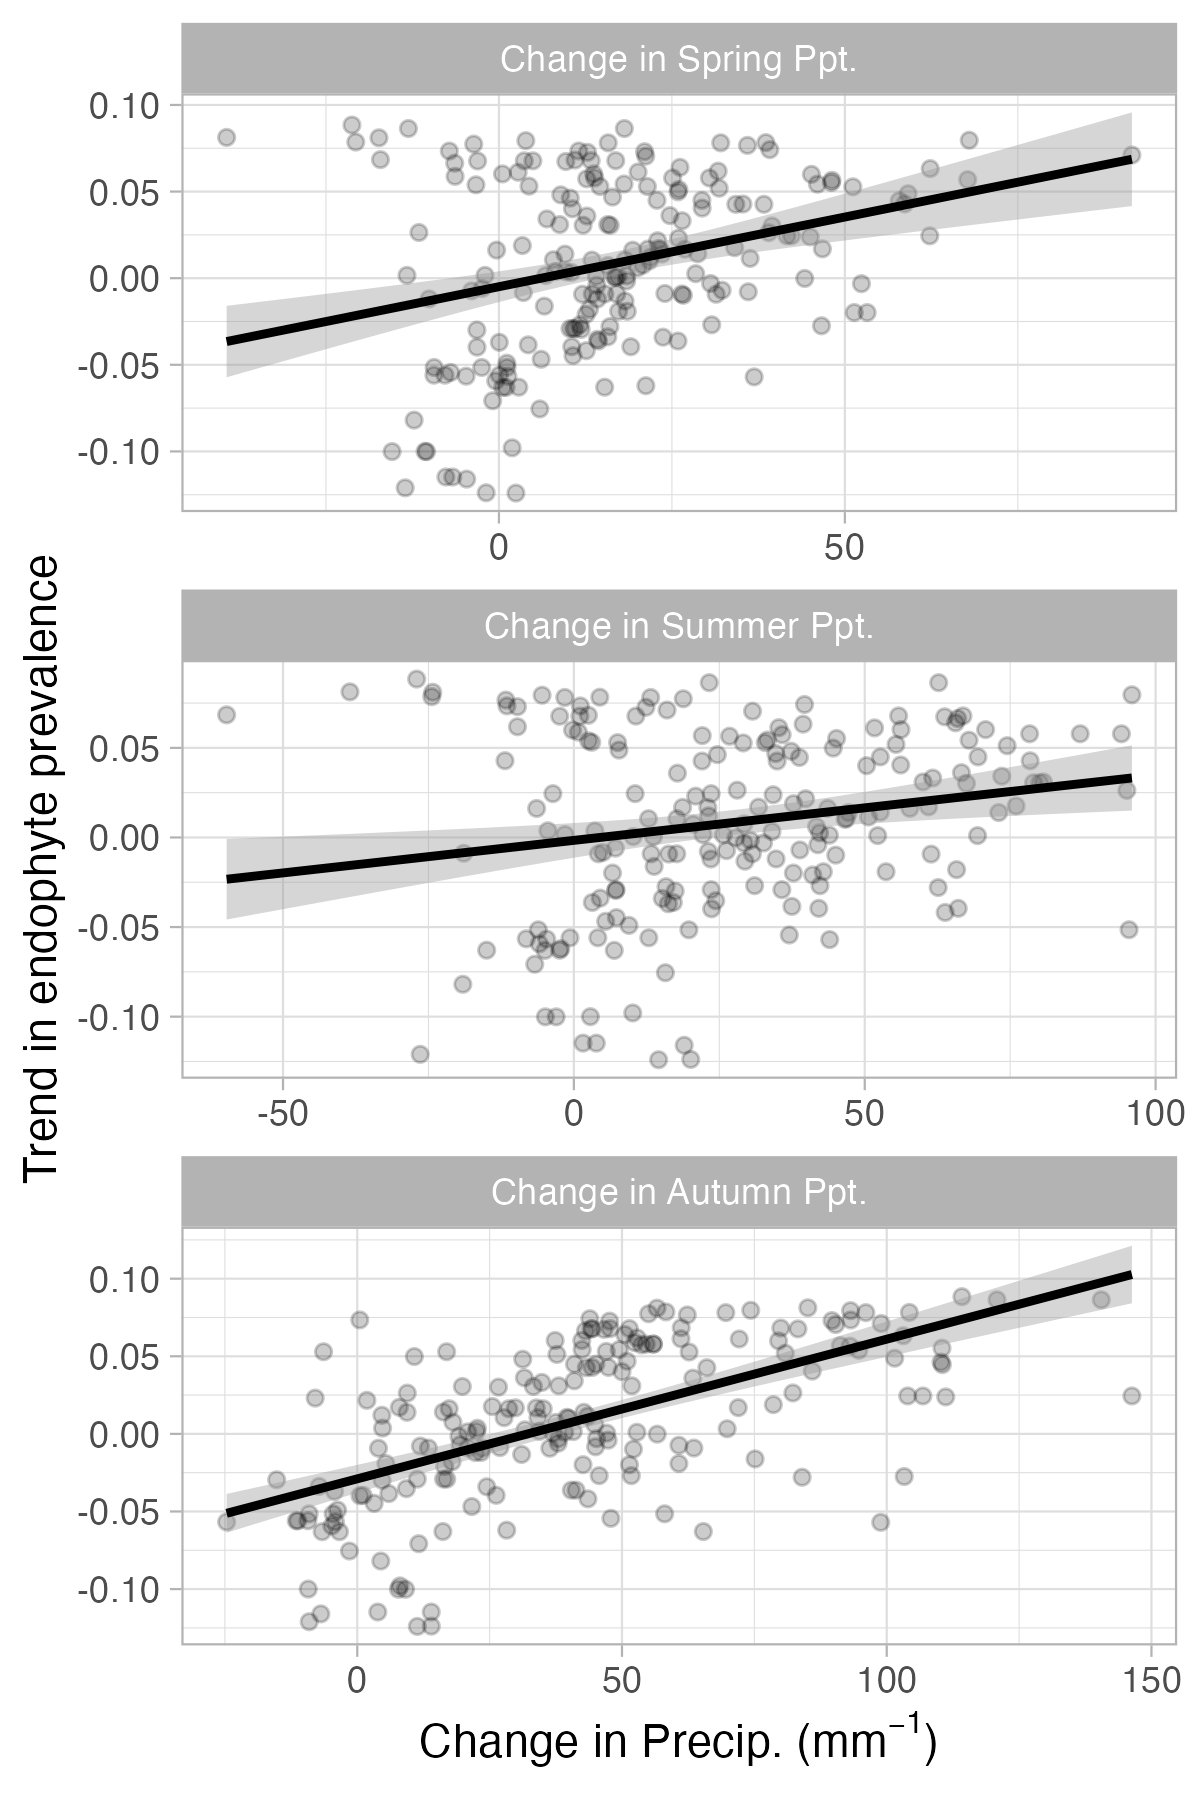
\includegraphics[width = .7\linewidth]{ppt_regression_plot_ESA.png}
	\caption{\textbf{Correlations between changes in climate drivers and changes in endophyte prevalence.} Color denotes the Spearman correlation coefficient between the relative rate of change in endophyte prevalence and the change in annual mean temperature ($^oC$) and total annual and seasonal precipitation (mm), as well as the change in the coefficient of variation of each climate driver. Positive correlation coefficients indicate that greater increases in a climate driver were associated with larger increases in endophyte prevalence, while negative values indicate that . Asteriks denote correlation coefficients $> .3$ or $< -.3$.}
\end{figure}


\begin{figure}[H]
	\centering
	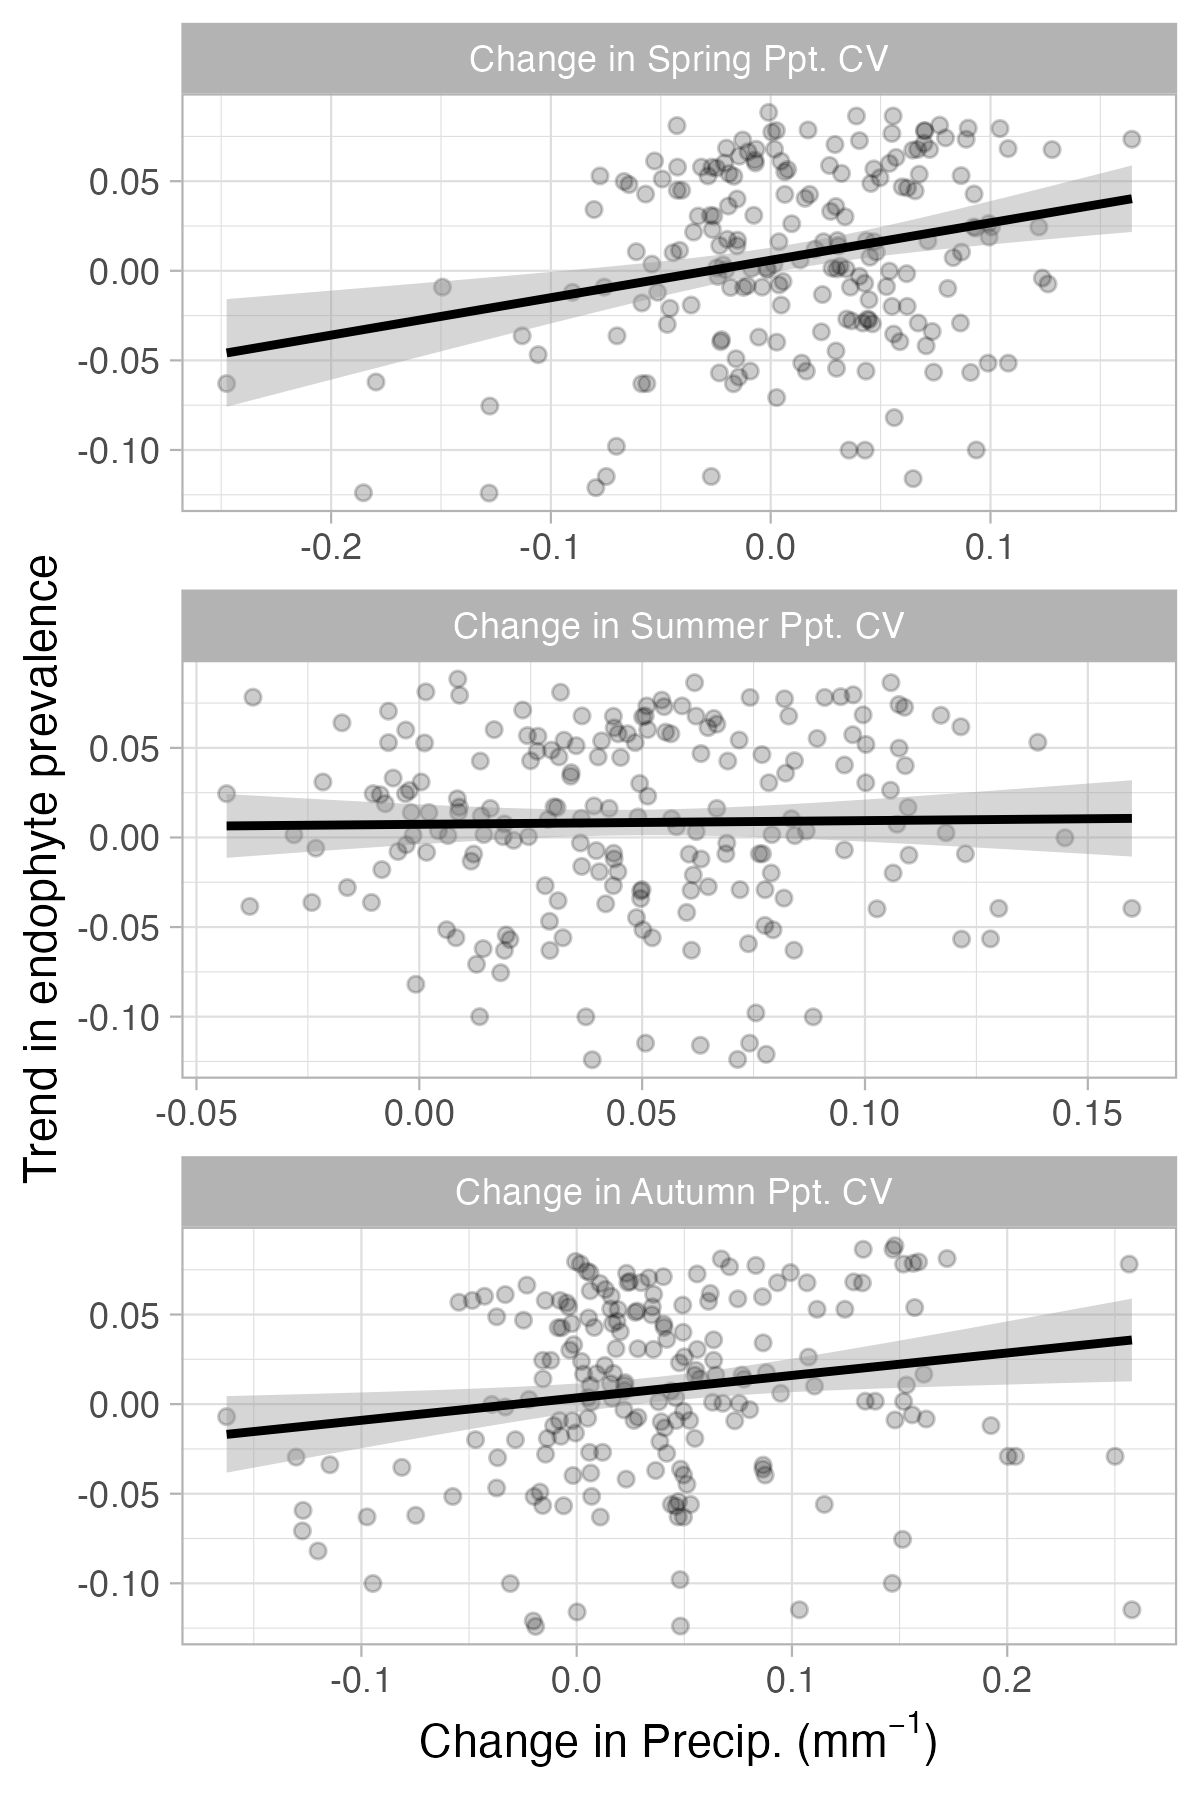
\includegraphics[width = .7\linewidth]{ppt_CV_regression_plot_ESA.png}
	\caption{\textbf{Correlations between changes in climate drivers and changes in endophyte prevalence.} Color denotes the Spearman correlation coefficient between the relative rate of change in endophyte prevalence and the change in annual mean temperature ($^oC$) and total annual and seasonal precipitation (mm), as well as the change in the coefficient of variation of each climate driver. Positive correlation coefficients indicate that greater increases in a climate driver were associated with larger increases in endophyte prevalence, while negative values indicate that . Asteriks denote correlation coefficients $> .3$ or $< -.3$.}
\end{figure}



\subsubsection*{Performance on test data}
We found that while the model predicts broader regional trends in endophyte prevalence present in the contemporary survey data such as declining endophyte prevalence towards western longitudes in \emph{A. hyemalis} (Fig. 6 B-C), however the contemporary data contains additional variability at smaller scales not captured by our sampling of herbarium specimens.
We interpreted this to mean that the model captured regional spatial dynamics, but underpredicts local scale dynamics. 
We discuss potential model improvements in the Discussion.

\begin{figure}[H]
	\centering
	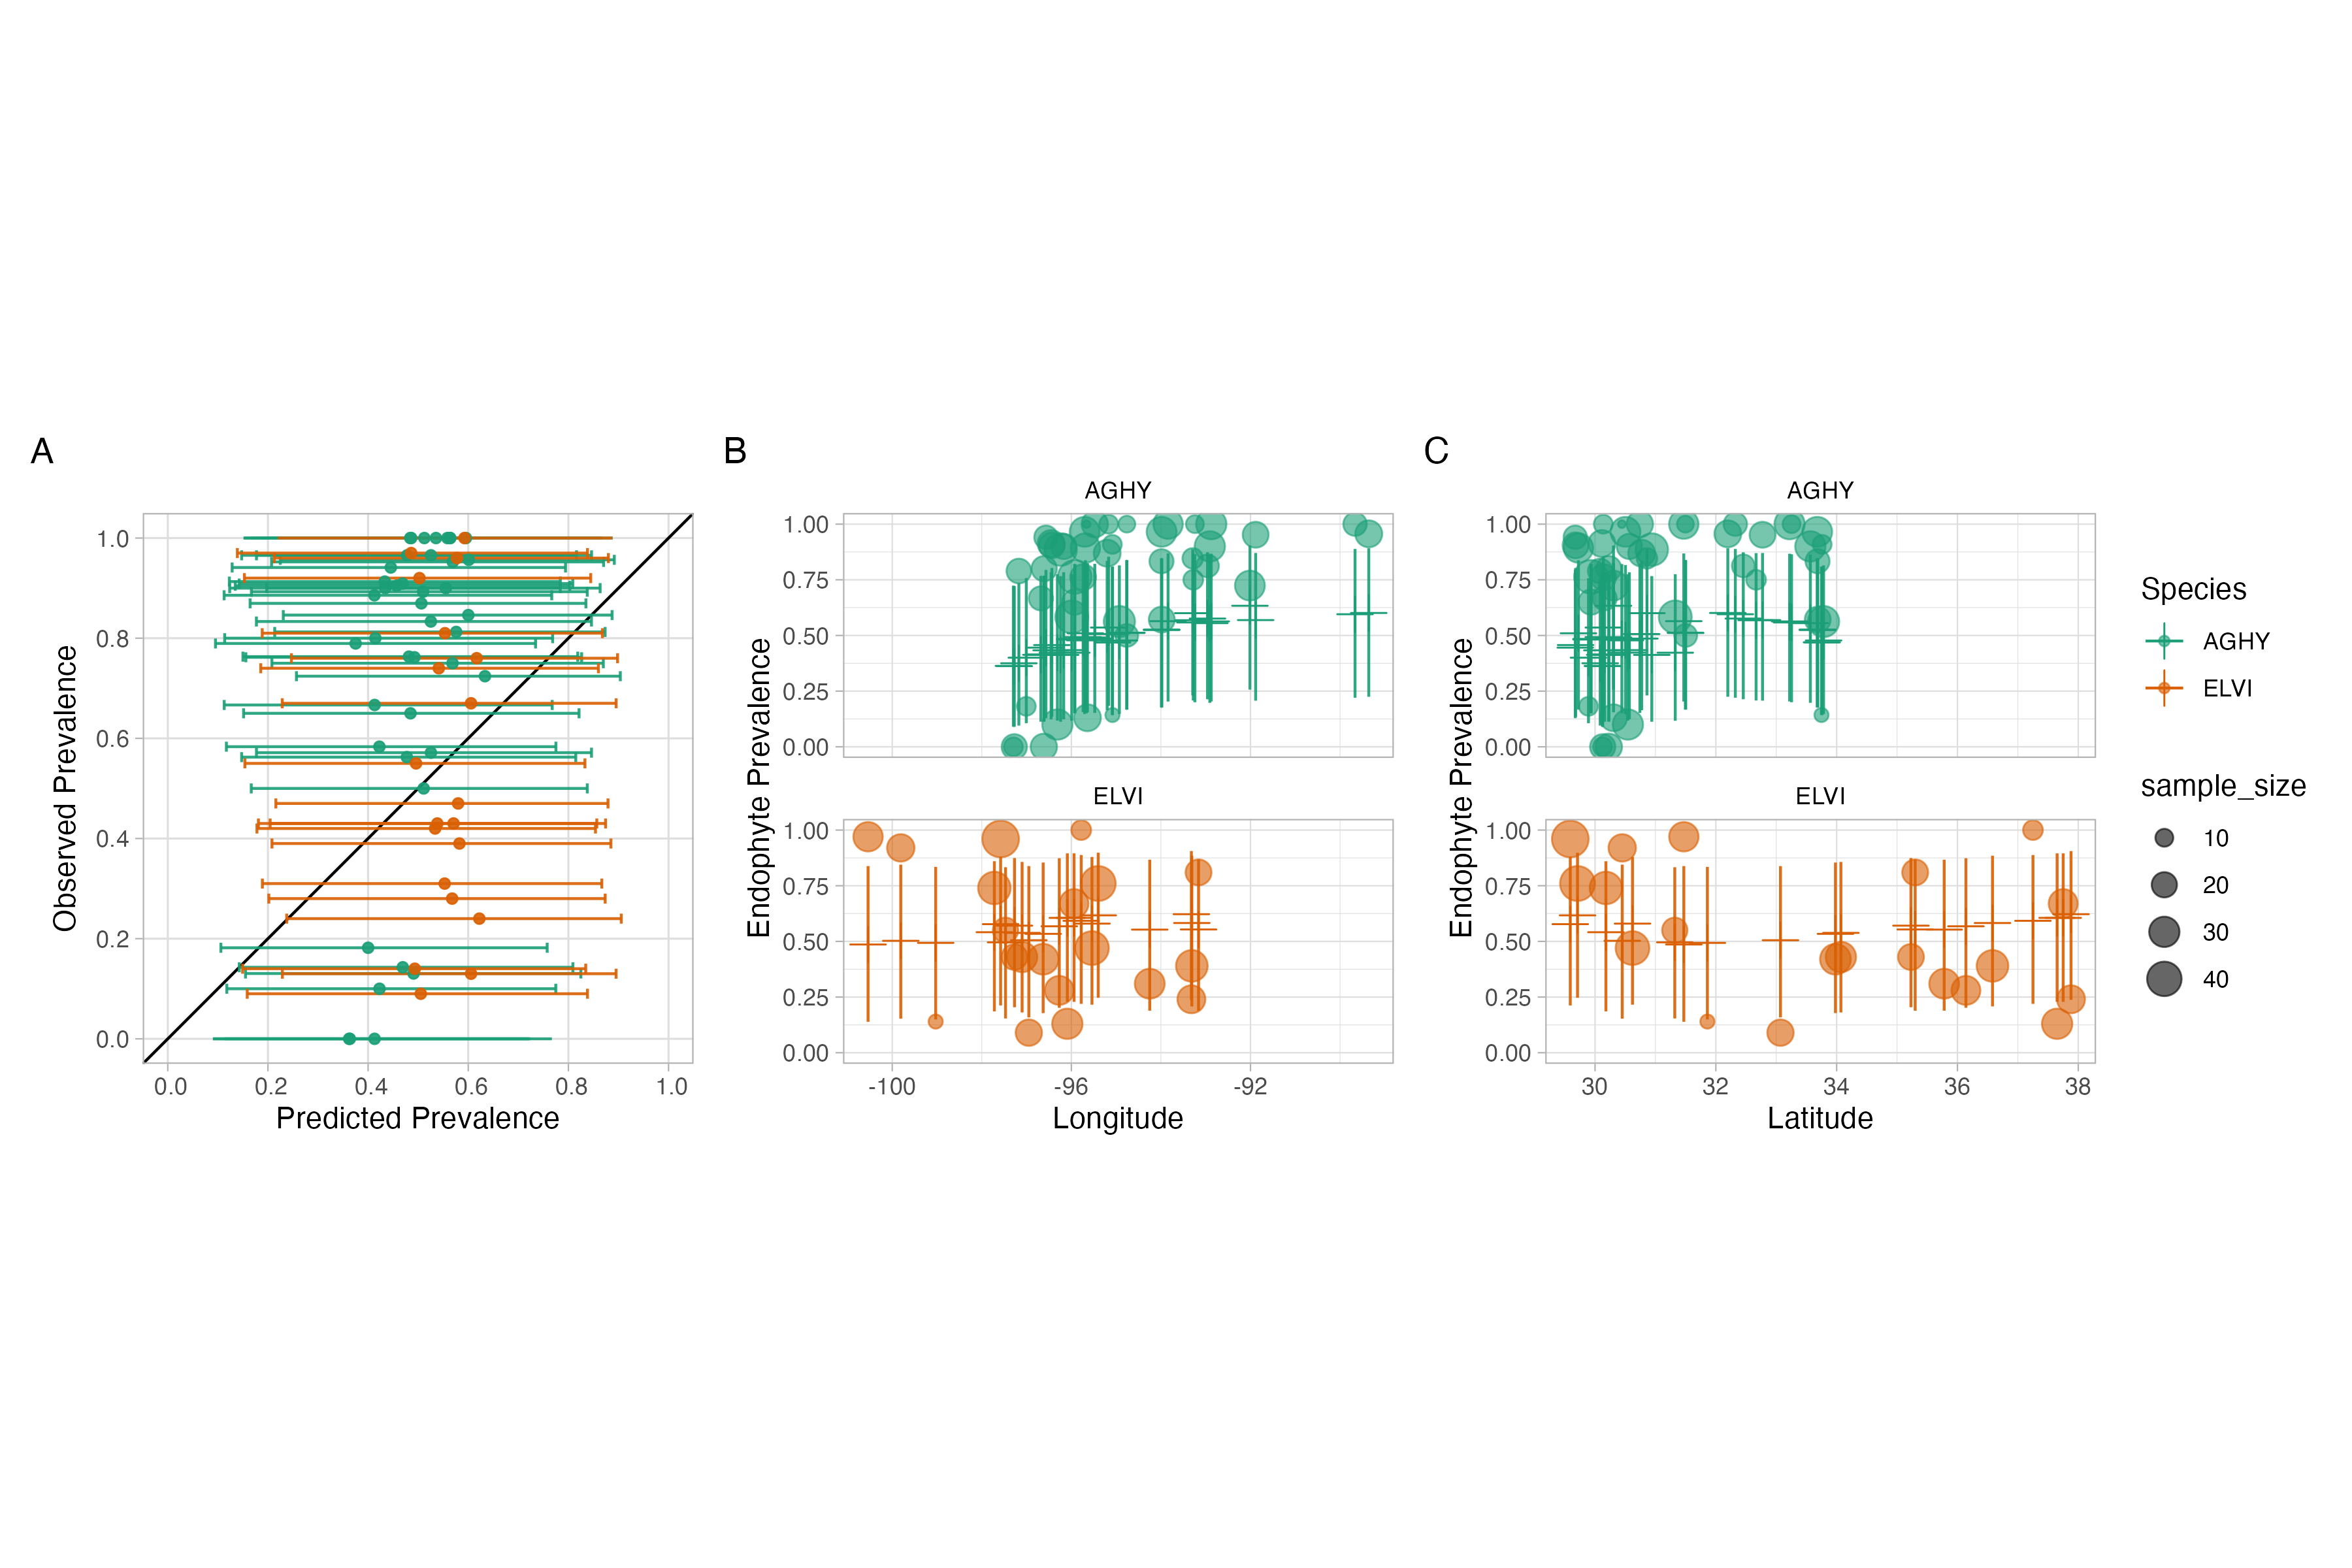
\includegraphics[width = \linewidth]{contemp_test_plot.png}
	\caption{\textbf{Predicted vs observed endophyte prevalence for contemporary test data.} (A) The model, trained on historic herbarium collection data, performed modestly at predicting contemporary endophyte prevalence in \emph{A. hyemalis}, as indicated by some overlap of predicted 95\% CI with the 1:1 line, however contemporary test data generally had more variance between populations than model predictions. The model did recapitulate broader regional trends across (B) longitude and (C) latitude. Point size in panels B and C reflect sample sizes of contemporary endophyte population surveys.}
\end{figure}

\section*{Discussion}
Our examination of historic plant specimens revealed a cryptic biotic reponse to climate change. 
For the three host species we examined, there have been clear increases in fungal endophyte prevalence over the last two centuries.
Increases in prevalence of \emph{Epichloë}, which are vertically transmitted, can potentially be interpreted as adaptive changes that improve the fitness of their hosts under stressful conditions.
This interpretation is in line with theory predicting that the positive fitness feedback caused by vertical transmission leads beneficial symbionts to rise in prevalence within a population \cite{fine1975vectors}.
We found that trends in endophyte prevalence varied across the distribution of each species in assocation with observed changes in climate drivers, suggesting that the endophytes have contributed to host resilience under environmental change.
Taken together, this suggests a strengthening of the mutualism over the last two centuries.


Differences between the responses of each host species underscore that while all of these $C_3$ grasses share similar broad-scale distributions, each engages in unique biotic interactions and has unique niche requirements.
We identified hotspots of change for \emph{A. perennans}, which experienced the strongest absolute changes in endophyte prevalence (Fig. 5).
Declines in the southern portion of its range and increases in the north suggest a potential poleward range shift of endophytic plants. 
Based on previous work demonstrating that endophytes can shield their hosts from drought stress \cite{decunta2021systematic}, we generally predicted that drought conditions could be a driver of increasing endophyte prevalence. 
In line with this expectation, increasing prevalence for this species was associated with decreasing precipitation, most strongly with autumn-season declines (Fig. 7). 
\emph{A. perennans} typically blooms in the autumn.
Endophytes could be playing a role helping hosts weather autumn-season droughts while the species is dormant. 
It may be useful to investigate whether lagged climate effects are important predictors of host fitness in this system \cite{evers2021lagged}. 
To our knowledge, the response of the symbiosis in \emph{A. perennans} to drought has not been examined experimentally, but in a greenhouse experiment, endophytes had a positive effect on host reproduction under shaded, low-light conditions \citep{davitt2010costs}. 
\emph{Epichloë} endophytes have been connected to a suite of non-drought related fitness benefits including herbivore protection \citep{brem2001epichloe}, salinity resistence \citep{wang2020effects}, and mediation of the soil microbiome \citep{roberts2015rhizosphere} 
These effects are potentially mediated by the diverse bioactive alkaloids and other signaling compounds they produce \citep{saikkonen2013chemical}.
The strong increase in symbiotic \emph{A. perennans} could be explained, at least in part, by these diverse benefits. 
\emph{A. hyemalis} experienced more consistently positive increases in endophyte prevalence related to changes in spring temperature and precipitation.  
This result is in line with previous work demonstrating drought benefits in a greenhouse manipulation with this species \citep{davitt2011understanding} that led us to expect  that endophyte prevalence should similarly increase at a greater rate in regions that have experienced increasing drought.
%It is possible that the study region has not experienced a magnitude of climate change great enough to cause larger changes in endophyte prevalence for this species. 
%Weak associations with drought could also be explained by climate-driven changes in the rate of imperfect transmission (the generation of non-symbiotic offspring from symbiotic hosts), which could counterbalance endophyte-mediated fitness benefits \citep{donald2021context}. 
For \emph{E. virginicus}, which experienced the most modest changes in endophte prevalence overall, we found a strong relationship between temporal trends and  changes in the mean and variability of temperature, as well as with decreases in summer precipitation.
Surveys by \citet{sneck2017variation}, used as part of the test data in this study, identified a drought index (SPEI) that integrates precipitation with estimated evapotranspiration as an important predictor of endophyte prevalence.
While we show consistent increasing trends in prevalence between the three species, the mechanisms that explain these changes may be diverse and idiosyncratic. 

Our spatially-explicit model predicted regions of both high and low endophyte prevalence, suggesting that symbiotic and non-symbiotic host plants have overlapping, but non-identical niche requirements.
Endophytes fitness benefits potentially explain the spatial distribution of prevalence by allowing their hosts to persist in environments where they otherwise could not \citep{afkhami2014mutualist, kazenel2015mutualistic}.
For example, fitness benefits of the symbiosis could explain high predicted prevalence in \emph{E. virginicus} towards the north or in \emph{A. hyemalis} towards its range center coinciding with strong environmental gradients.
Previous population surveys for endophytes, which were used as test data for our model, found similar latitudinal trends in prevalence in these species \citep{sneck2017variation,rudgers2009benefits}, but at smaller scales. 
While the model recreated these large-scale spatial trends, test data was more variable. 
Using test data to validate our model predictions allows us to evaluate places to improve the model's ability to perform well at out-of-sample prediction, which will be particularly important for predicting host and symbiont niche-shifts under future climate change.
Lack of information on local variability may simply be a feature of data derived from herbarium specimens. 
Even though they are samples from local populations, they are single specimens that are aggregated over in broad-scale model estimates.
Poor predictive ability at local scales in this grass-endophyte system is not surprising, as previous studies have found that local variation, even to the scale of hundreds of meters can structure endophyte-host niches \cite{kazenel2015mutualistic}. 
\citet{sneck2017variation} also identified host genotype as an important predictor of endophyte prevalence in \emph{E. virginicus}.
Other studies have found factors including land-use history \cite{vikuk2019infection} and the biotic environment, including herbivory \cite{rudgers2016long}, to be important predictors of endophyte ecology.
Incorporating available climatic and soil layers as covariates is an obvious first step that could improve predictions.
Towards the goal of predicting the dynamics of microbial symbioses under climate change, models that integrate data from local and regional scales would be an important step to bridge the gap that often exists between large but broad bioclimatic and biodiversity data and small but local data on biotic interactions.  \cite{miller2019recent, isaac2020data}


Our analysis advances the use of herbarium specimens in global change biology in two ways. 
First and foremost, this is the first study to link long-term changes in microbial symbioses to changes in climate using specimens from natural history collections.
The responses of microbial symbioses are a rich target for future studies within museum specimens, particularly those that take advantage of advances in sequencing technology.
While we used relatively coarse presence/absence data based on fungal morphology, other studies have examined historic plant microbiomes using molecular sequencing and sophisticated bioinformatics techniques, but these studies have so far been limited to relatively few specimens at limited spatial extents \cite{yoshida2015computational, heberling2019utilizing, bieker2020metagenomic, gross2021hidden, bradshaw2021global}. 
Continued advances in capturing historic DNA and in filtering out potential contamination during specimen storage \citep{daru2019novel, bakker2020herbarium, raxworthy2021mining} will be imperative in the effort to scale up these efforts. 
This scaling up will be essential to be able to quantify changes not just in the prevalence of symbionts, but also in symbionts' intraspecific variation and evolutionary responses to climate change, as well as  in changes in the wider microbial community. 
Answering these questions as well as the unknown questions that future researchers may ask also reiterates the value in capturing meta-information during ongoing digitization efforts at herbaria around the world and during the accession of newly collected specimens \citep{lendemer2020extended}.
Second, we accounted for several potential biases in the data observation process that may be common to many collections-based research questions by using a spatially-explicit random effects model. 
Spatial autocorrelation \cite{willems2022forest}, potential biases introduced by the sampling habits of collectors \citep{daru2018widespread}, and variation between contemporary researchers during the collection of trait data, if not corrected for could lead to over-confident inference about the strength and direction of historic change.
Previous studies that have quantified the effects of collector biases typically find them to be small  \cite{davis2015herbarium,meineke2019herbarium}, and we similarly did not find that collector has a strong effect on the results of our analysis.
Fitting this model in a Bayesian framework allows for full propagation of uncertainty.

Ultimately, a central goal of global change biology is to generate predictive insights into the future of natural systems. 
While this survey of historic endophyte prevalence is necessarily correlative, it serves as a foundation to develop better predictive models of the response of microbial symbioses to climate change. 
Combining the insights from this type of regional-scale survey with field experiments and physiological data could be invaluable. 
While we found that climate is strongly correlated with endophytes' temporal responses, we do not know why trends in prevalence were weak in some areas or how endophytes would respond to more extreme changes in climate.
For example, transplanting symbiotic and non-symbiotic plants beyond the range edge of \emph{A. hyemalis} could tell us whether persistent low endophyte prevalence in that area is a result of environmental conditions that lead the symbiosis to negative fitness consequences, or is a result of some historical contingency or dispersal limitation that has thus far limited the presence of symbiotic hosts from a region where they would otherwise flourish and provide resilience.
While we observed evidence of mutualism resilience, more extreme environmental changes than those observed in our study could potentially push one or both partners beyond their physiological limit, leading to the collapse of the mutualism. 
Our analysis thus far is agnostic to changes in the distributions of hosts. 
Mechanistic models could connect the responses of both host and symbionts to abiotic climate drivers integrating dispersal processes. 
Beyond host-microbe symbioses, building these types of models would work towards quantitatively attributing biotic responses to anthropogenically driven climate change, similar to methods in climate science and economics \citep{stott2010detection, carleton2016social}.
%Elymus genotype
%Agrostis weedy



	%%%%%%%%%%%%%%%%%%%%%
	% Acknowledgments
	%%%%%%%%%%%%%%%%%%%%%
	% You may wish to remove the Acknowledgments section while your paper 
	% is under review (unless you wish to waive your anonymity under
	% double-blind review) if the Acknowledgments reveal your identity.
	% If you remove this section, you will need to add it back in to your
	% final files after acceptance.
	
	\section*{Acknowledgments}
	We thank Jessica Budke for help in drafting our initial destructive sampling plan, and to the many members of herbarium staff who facilitated our research visits, as well as to the hundreds of collectors who contributed to the natural history collections. 
	Several high schooler and undergraduate researchers contributed to data collection, including A. Appio-Riley, P. Bilderback, E. Chong, K. Dickens, L. Dufresne, B. Gutierrez, A. Johnson, S. Linder, E. Scales, B. Scherick, K. Schrader, E. Segal , G. Singla, and M. Tucker.
	This research was supported by funding from National Science Foundation (grants 1754468 and 2208857) and by funding from the Texas Ecolab Program.


	%%%%%%%%%%%%%%%%%%%%%
	% Statement of Authorship
	%%%%%%%%%%%%%%%%%%%%%
	% This section should also be commented out while your MS is undergoing
	% double-blind review. The specifics should of course be adapted to
	% your paper, but the paragraph below gives some hints of possible
	% contributions.
	
	\section*{Statement of Authorship}
	

	
	\section*{Data and Code Availability}
	
	On initial submission, you may use this section to provide a URL for editors and reviewers that is `private for peer review'. After acceptance, this section must be updated with correct, working DOIs for data deposits (typically on the Dryad Digital Repository, ) and code deposits (such as in Zenodo). 
	
	\section*{Appendix A}
	\renewcommand{\thefigure}{A\arabic{figure}}
	\setcounter{figure}{0}
	
		\renewcommand{\thetable}{A\arabic{table}}
	\setcounter{equation}{0}  % reset counter 
	\setcounter{figure}{0}
	\setcounter{table}{0}
	
	\begin{figure}[H]
		\centering
		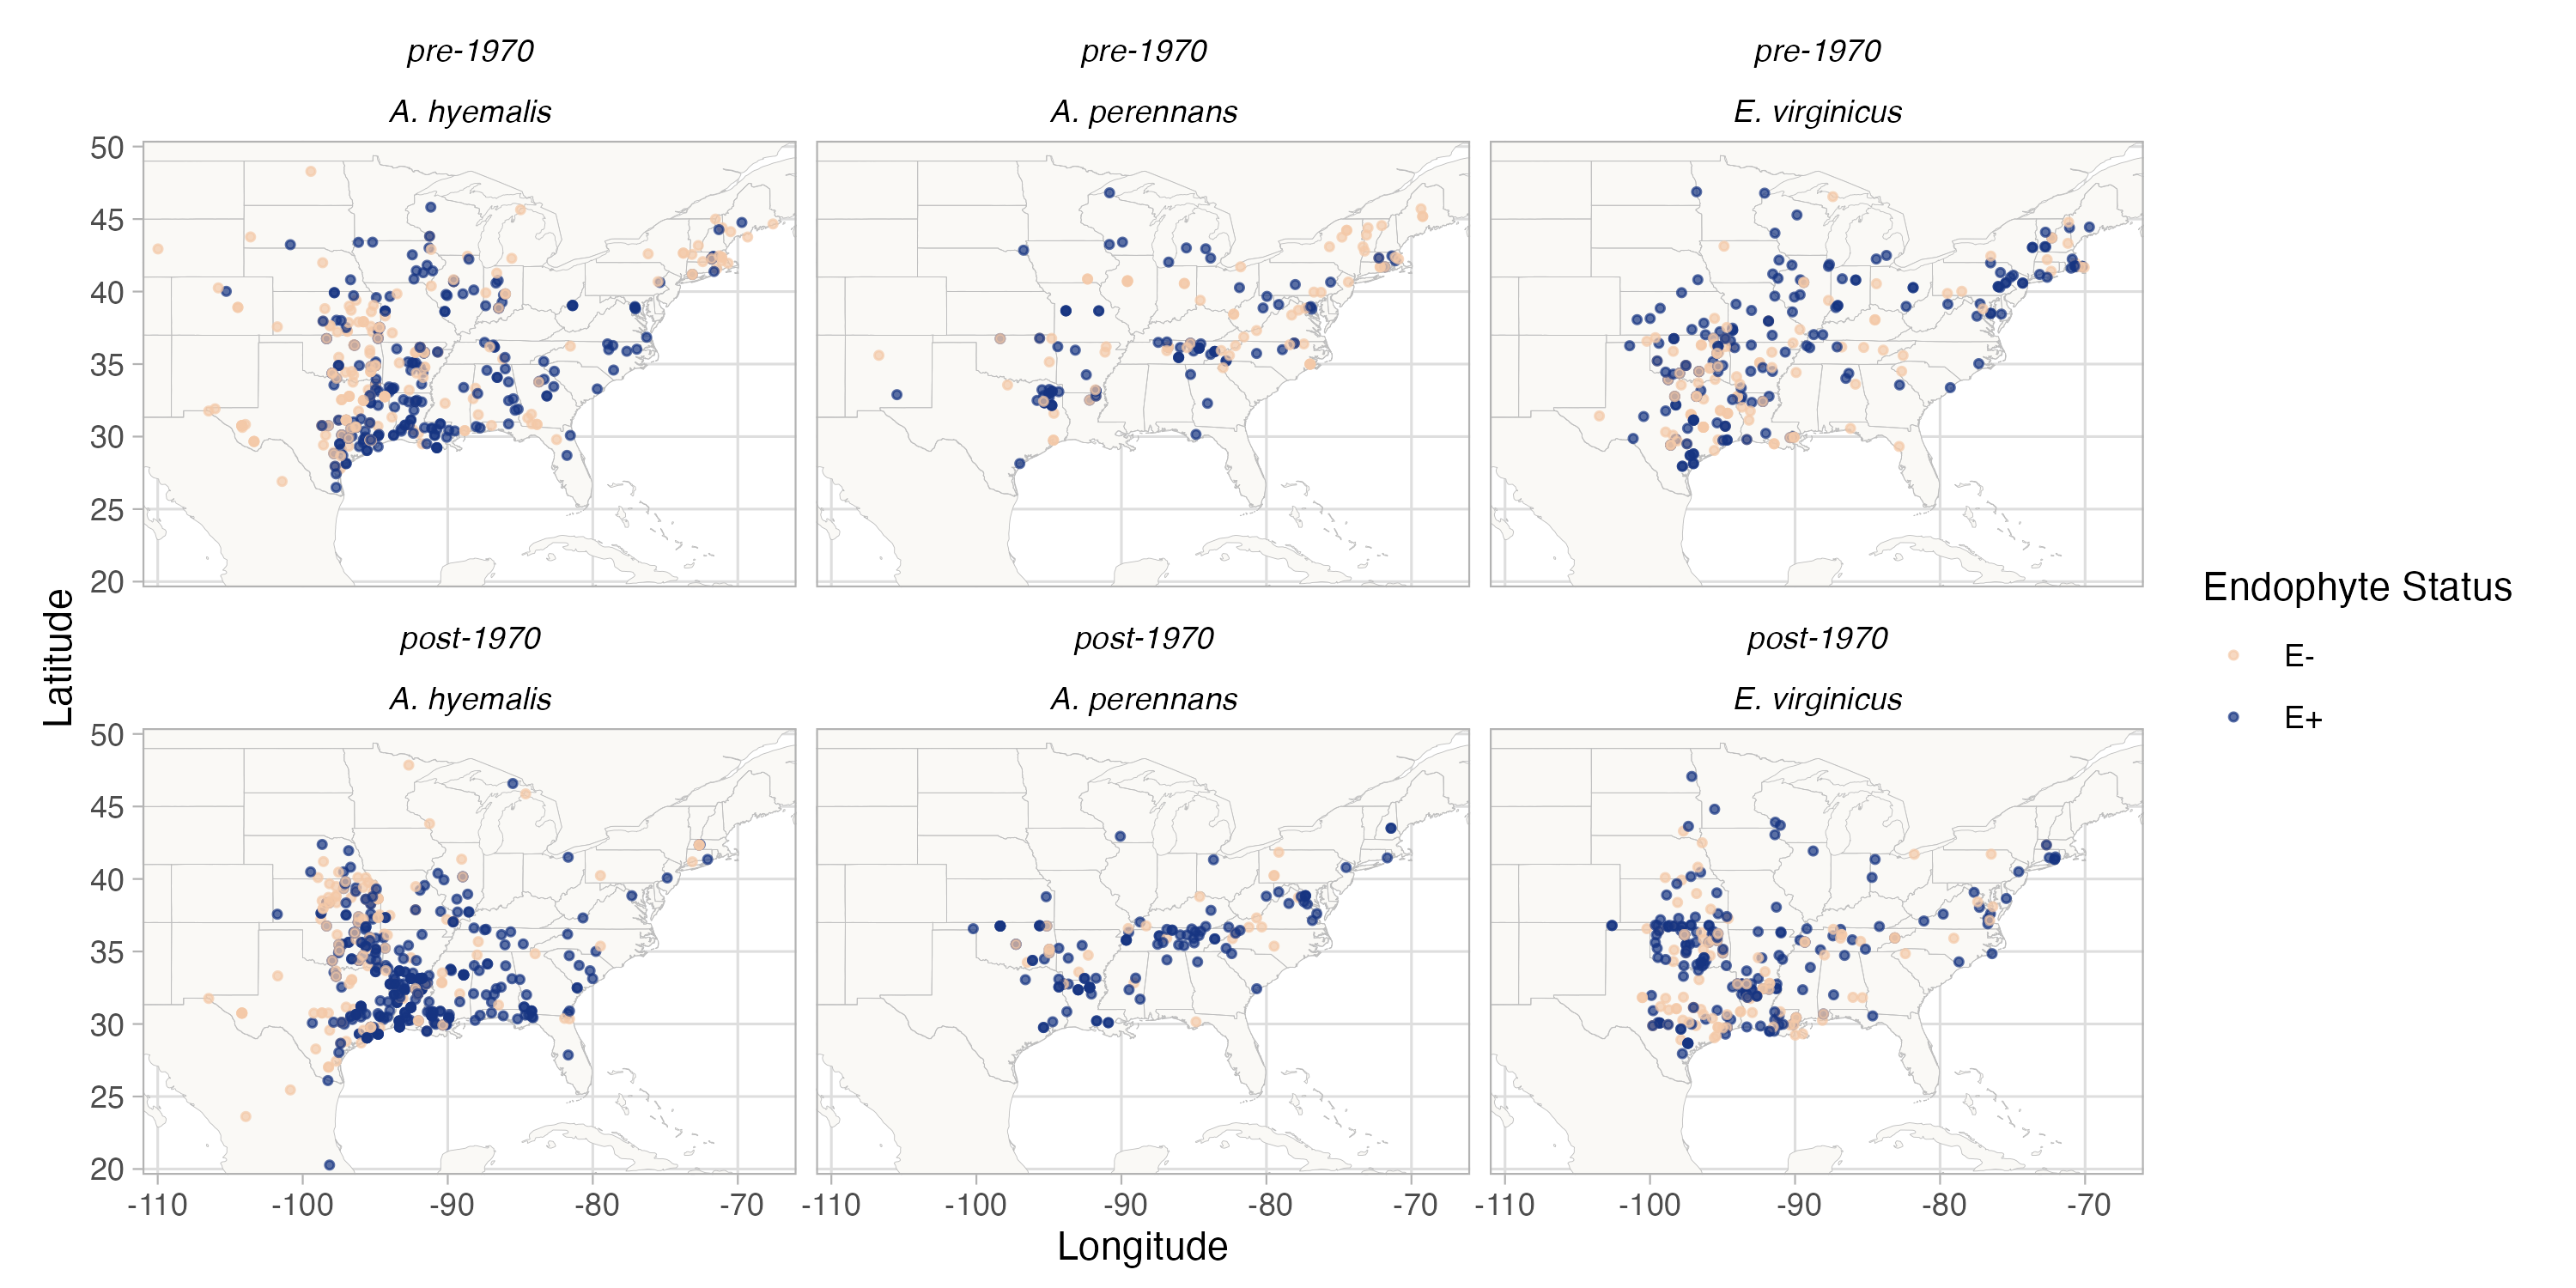
\includegraphics[width = \linewidth]{endo_status_map.png}
		\caption{\textbf{Endophyte presence/absence in specimens of each host species.} Points show collection locations colored according to whether the specimen contained endophytes ( E+; blue points) or did not contain endophytes (E-, tan points) and are faceted based on collection period.}
	\end{figure}
	
	\begin{figure}[H]
		\centering
		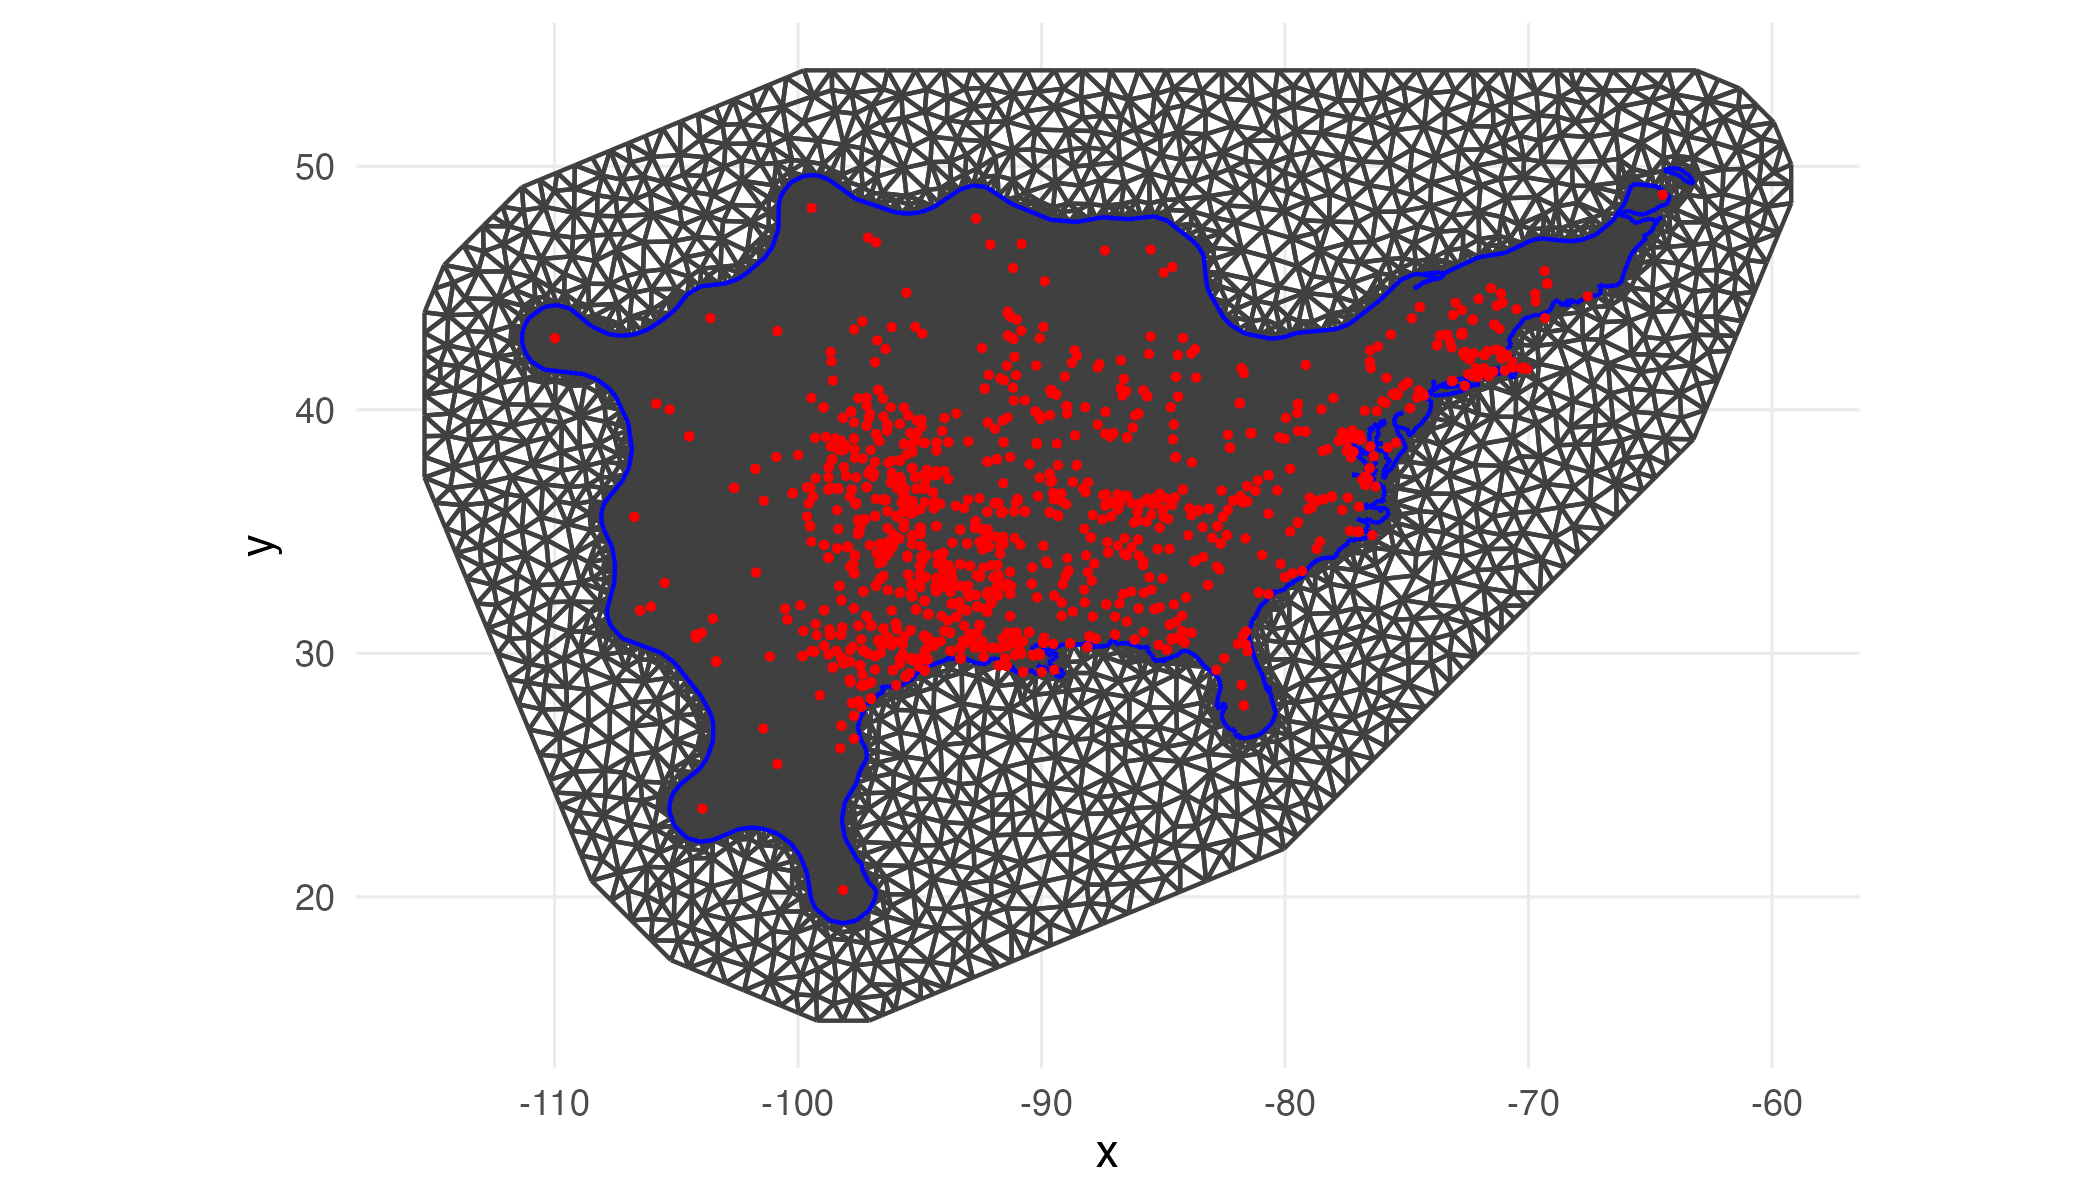
\includegraphics[width = \linewidth]{mesh_plot.png}
		\caption{\textbf{Delauney triangulation mesh used to estimate spatial dependence between data points}. Grey lines indicate edges of triangles used to define distances between observations. Red points indicate locations of sampled herbarium specimens, and the blue outlines show the international borders used to define the edge of the mesh along coastlines.}
	\end{figure}

\begin{figure}[H]
	\centering
	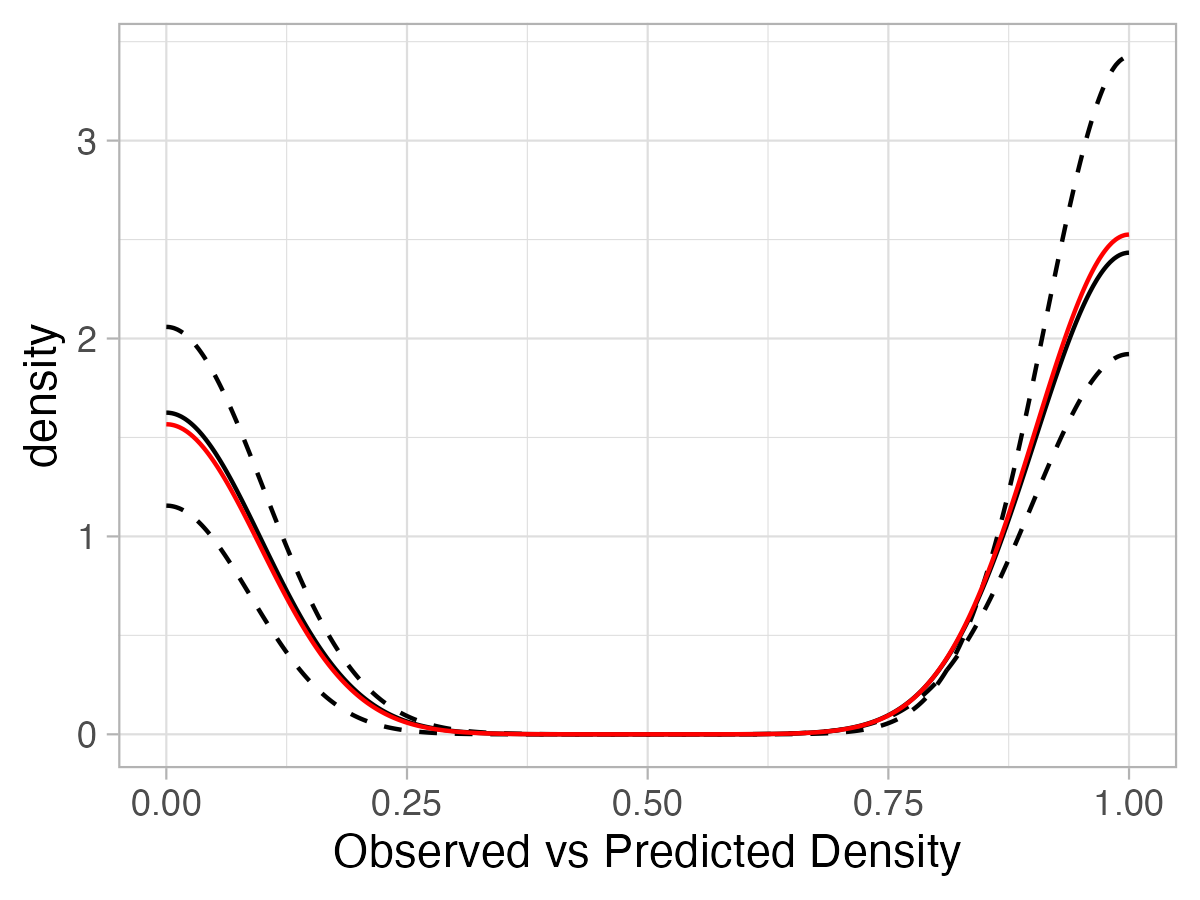
\includegraphics[width = .8\linewidth]{density_plot.png}
	\caption{\textbf{Consistency between real data and simulated values indicate that the fitted model accurately describes the data}. Graph shows density curves for the observed data (red) along with the mean(solid) and 95\% CI (dashed) of simulated values (black).}
\end{figure}

	
	\begin{figure}[H]
		\centering
		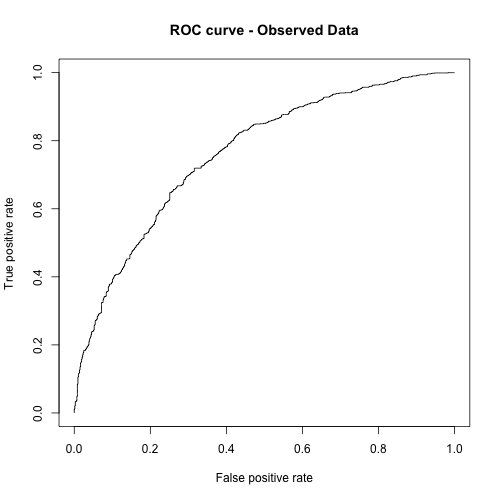
\includegraphics[width = .5\linewidth]{ROC_plot.png}
		\caption{\textbf{ROC plot showing model performance classifying observations according to endophyte status.} The curves show adequate model performance for observed (top) and test (bottom) data. The AUC for each is 0.77.}
	\end{figure}

\begin{figure}[H]
	\centering
	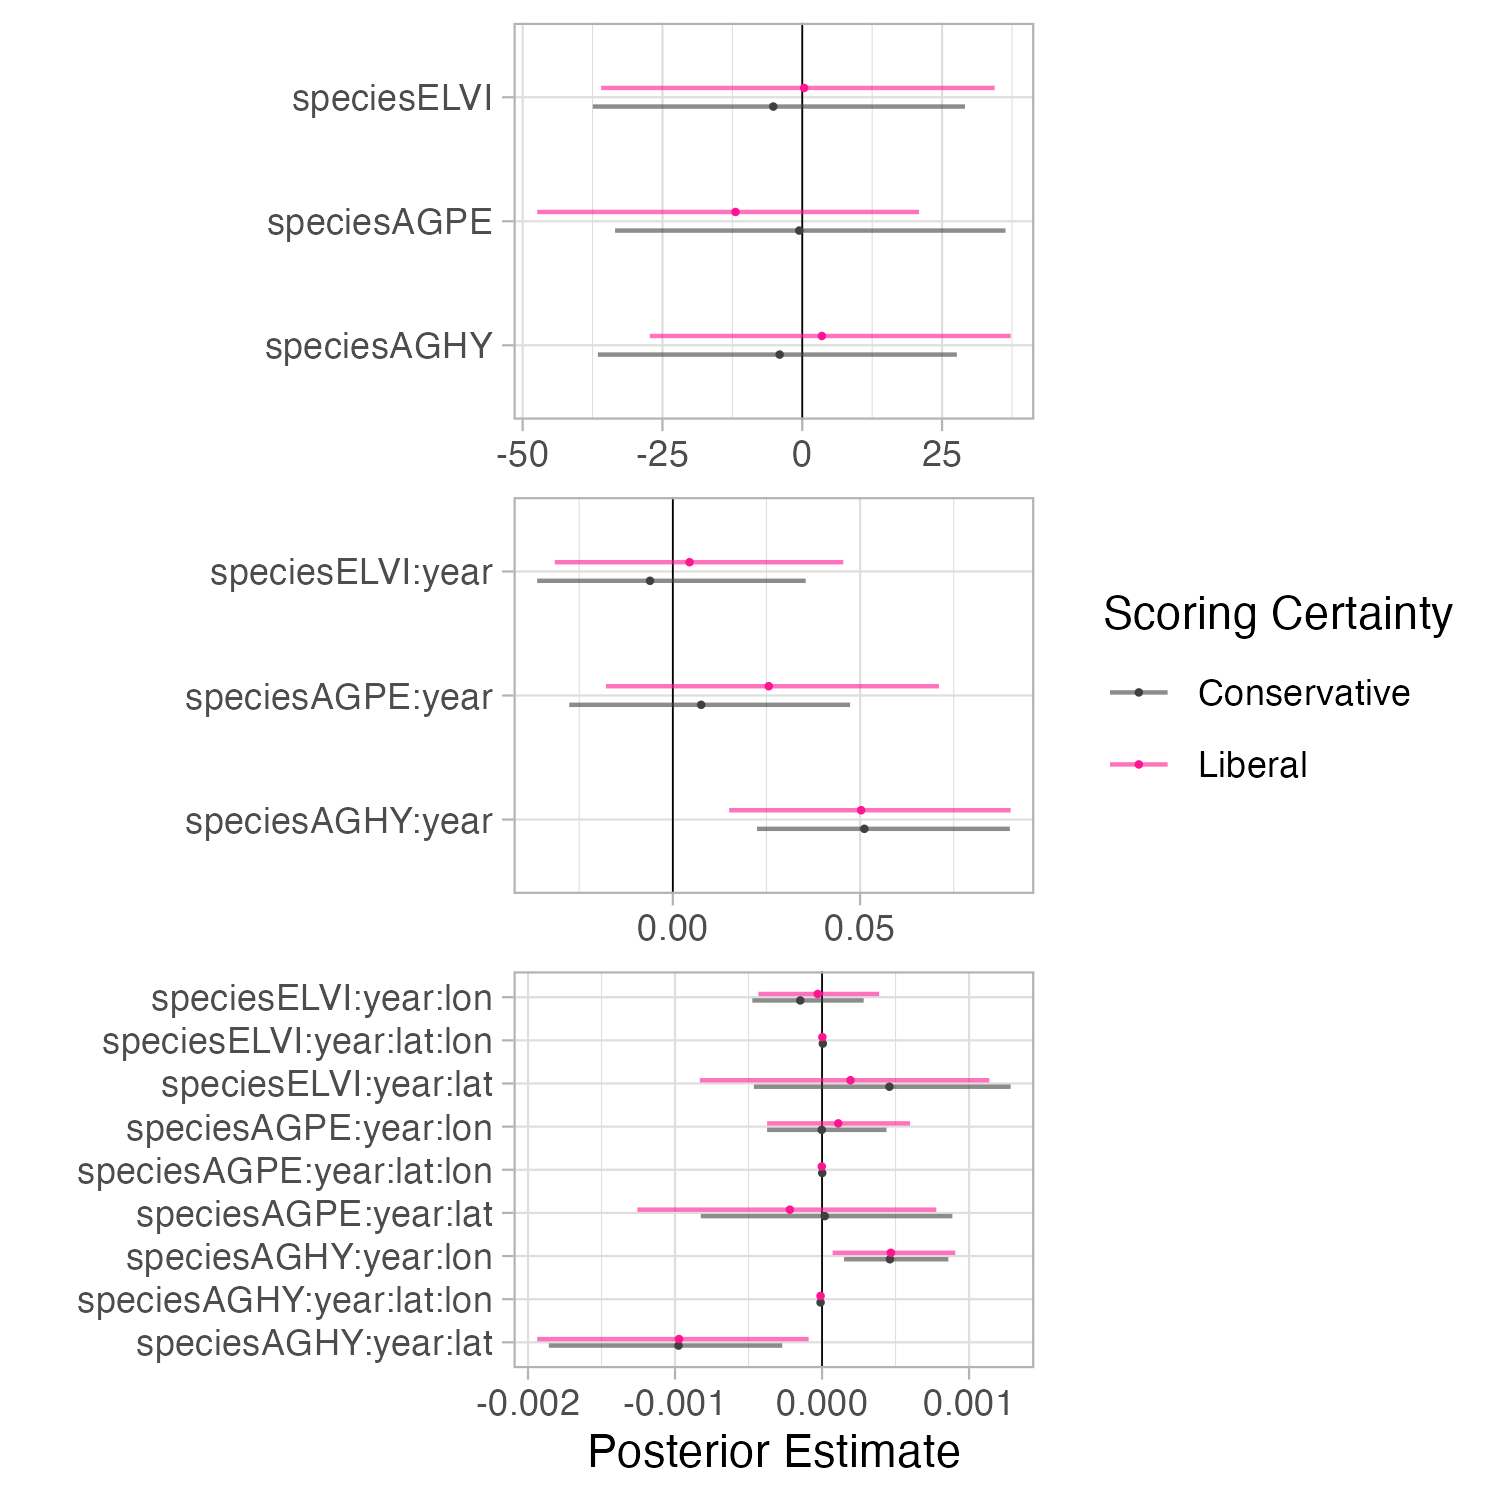
\includegraphics[width = \linewidth]{fixed_plot.png}
	\caption{\textbf{Comparison of posterior estimates of fixed effects when using Liberal or Conservative endophyte scores.}}
\end{figure}

\begin{figure}[H]
	\centering
	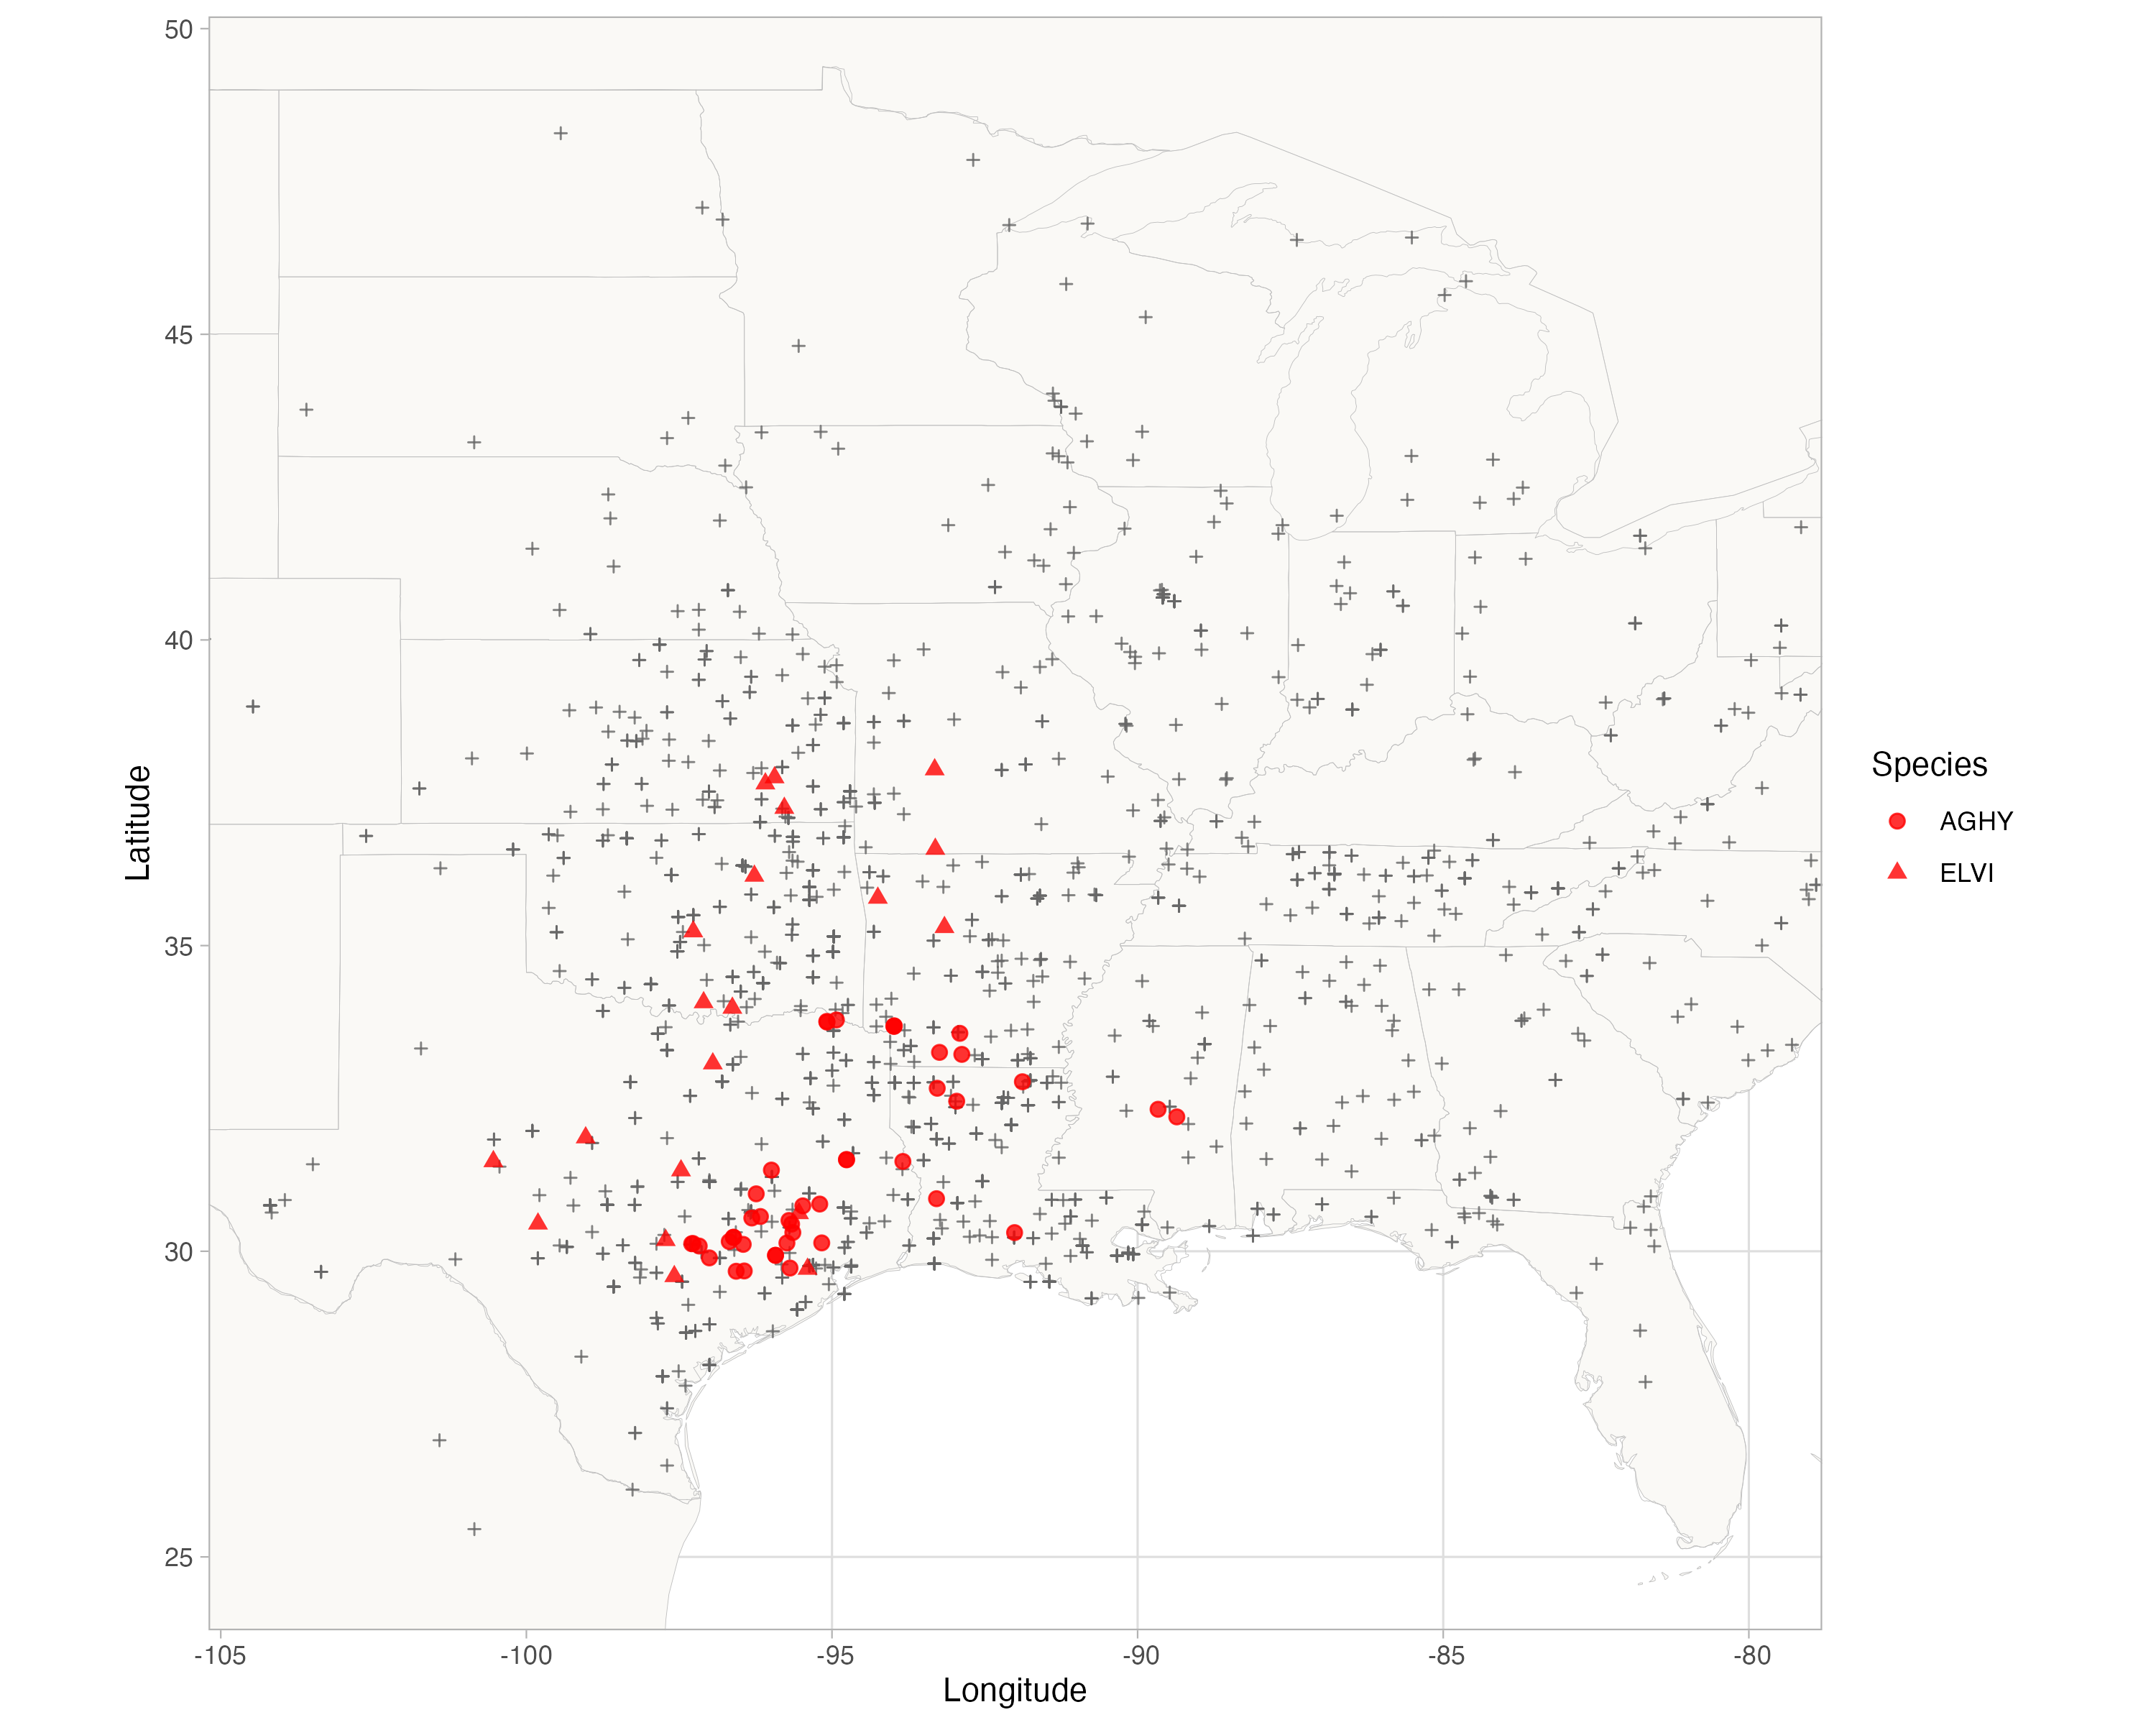
\includegraphics[width = \linewidth]{test_data_map.png}
	\caption{\textbf{Locations of contemporary surveys of endophytes in \emph{A. hyemalis} used as "test" data (red points), relative to the historical collection data (black crosses).}}
\end{figure}

	\begin{figure}[H]
	\centering
	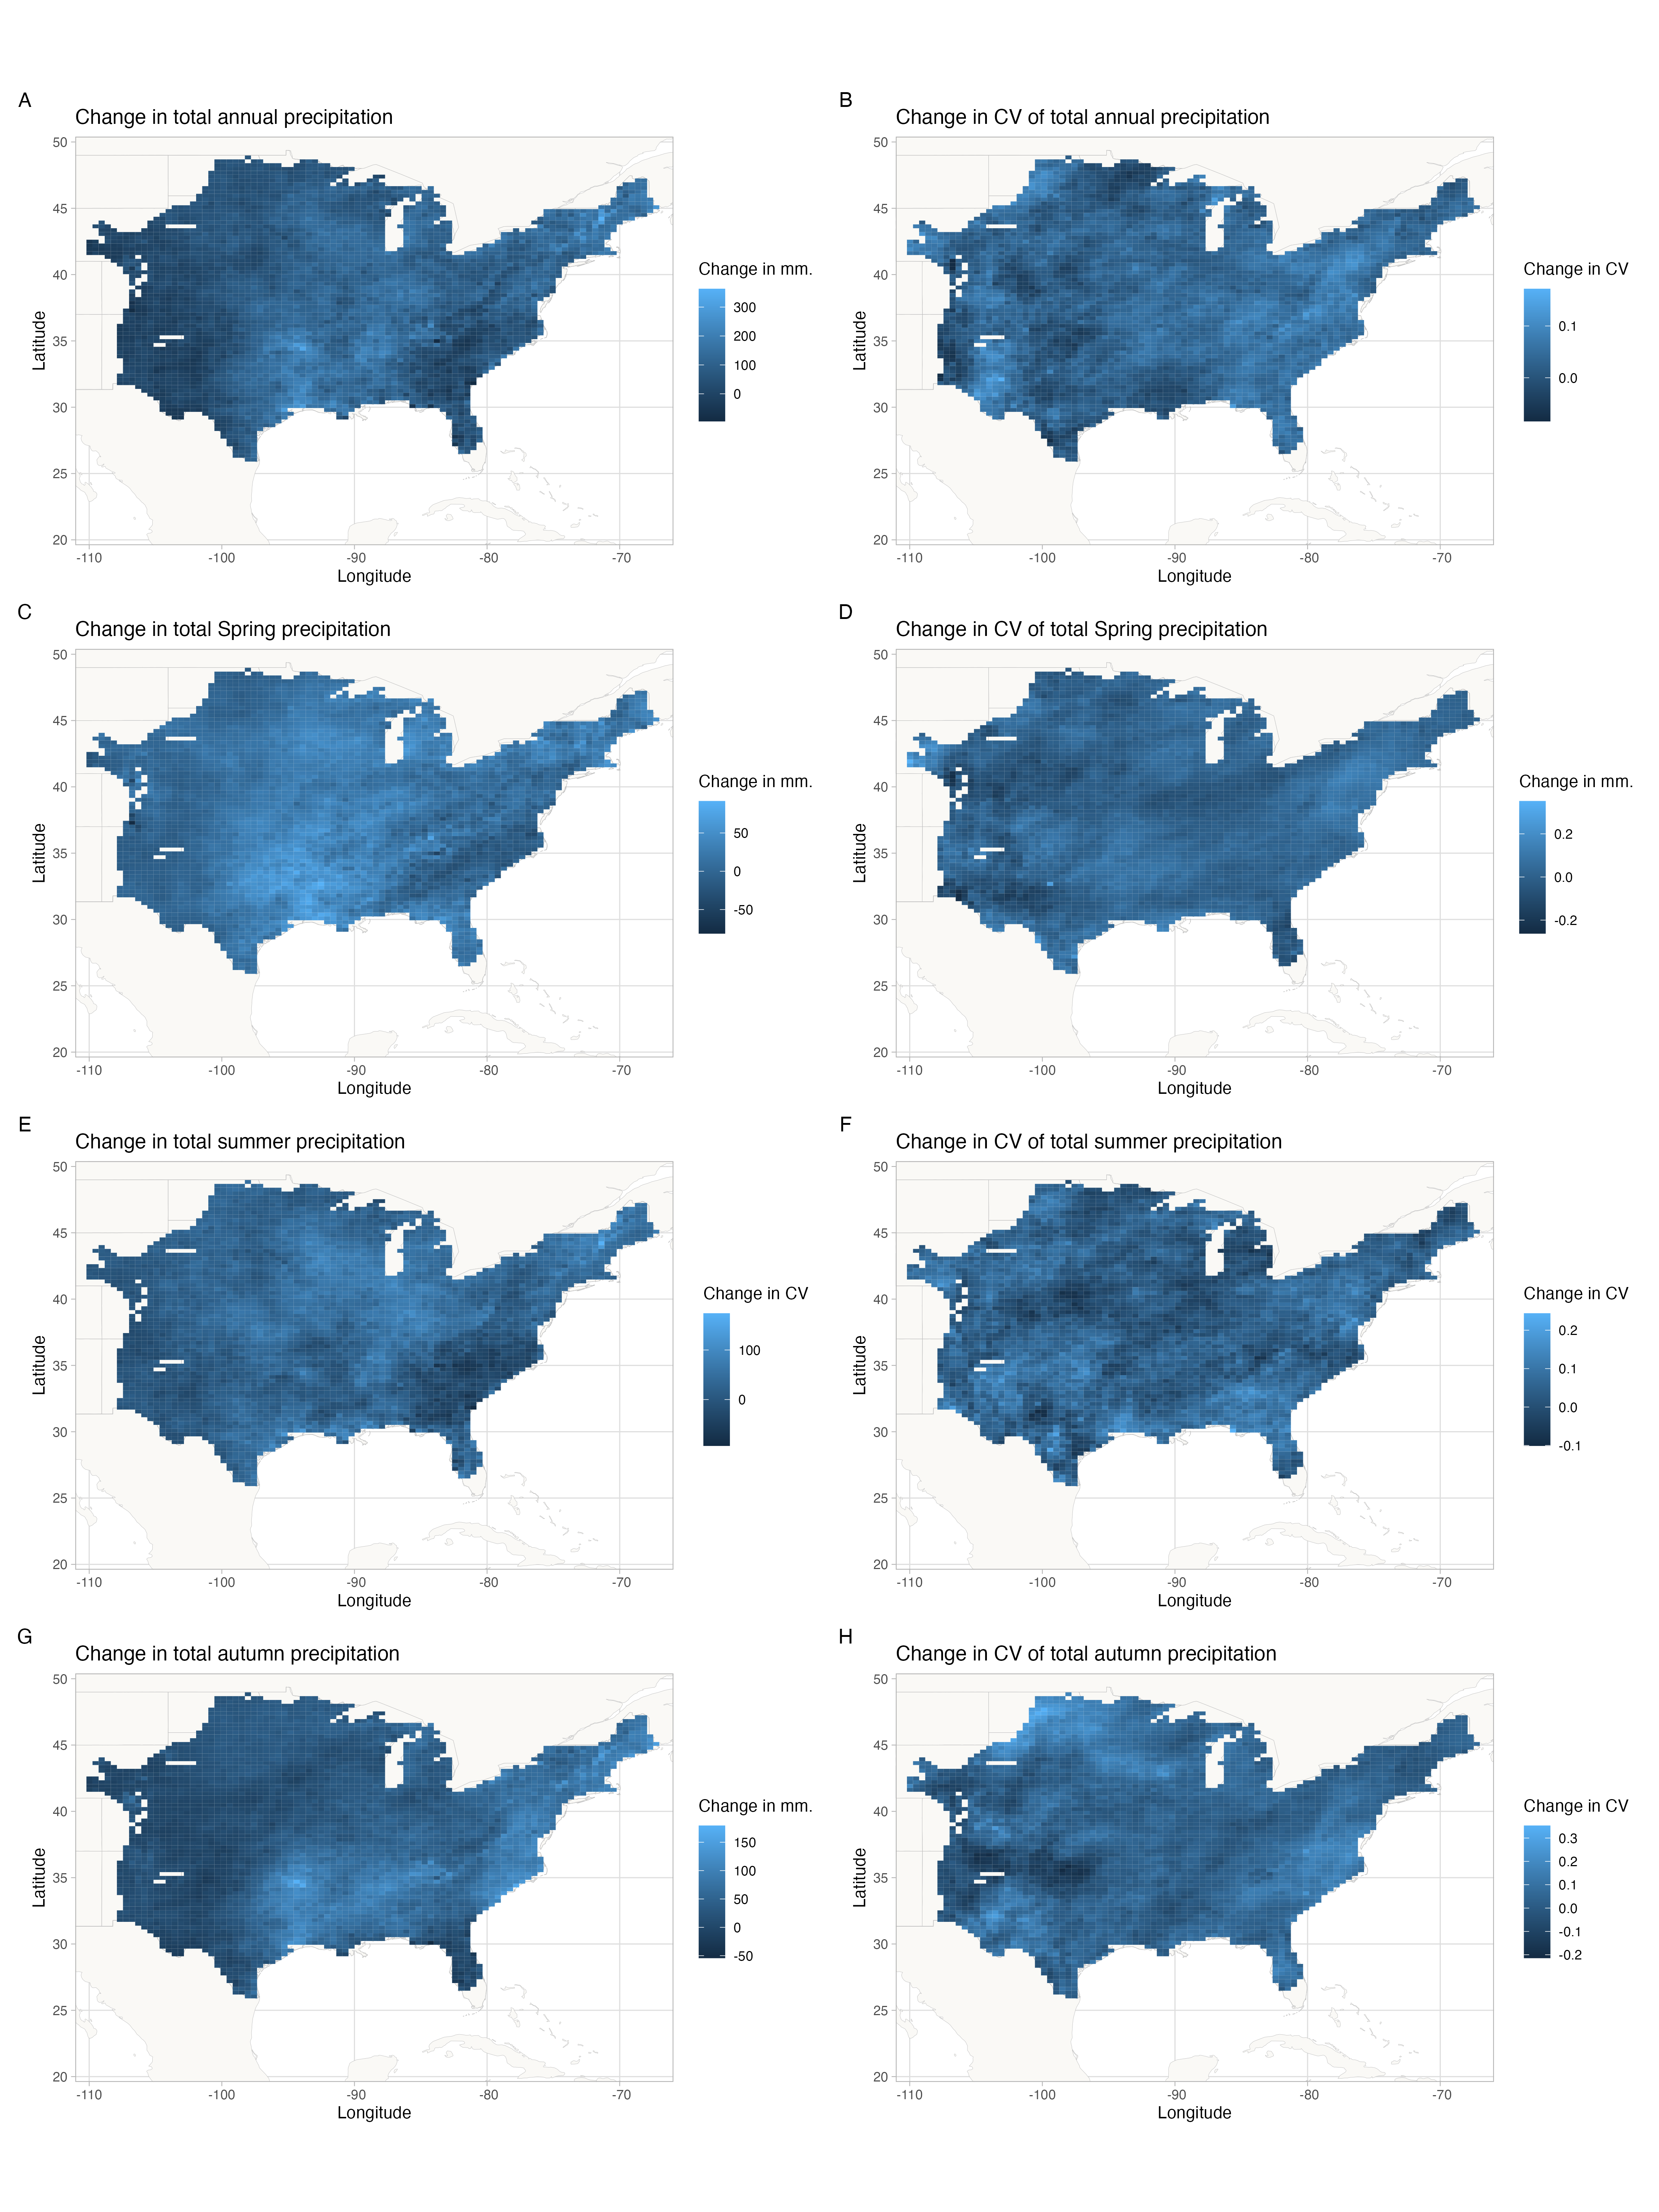
\includegraphics[width = .8\linewidth]{ppt_change_maps.png}
	\caption{\textbf{Change in precipitation between the periods 1895-1925 and 1990-2020.} Color represents change in annual or seasonal total precipitation (A,C,E,G) and in the coeffiecient of variation of annual or seasonal total precipitation (B,D,F,H). Maps show the study area of \emph{A. hyemalis}. Map pixels used in correlation analysis with endophyte change were pulled from studies areas specific to each host species. }
\end{figure}

	
	\begin{figure}[H]
		\centering
		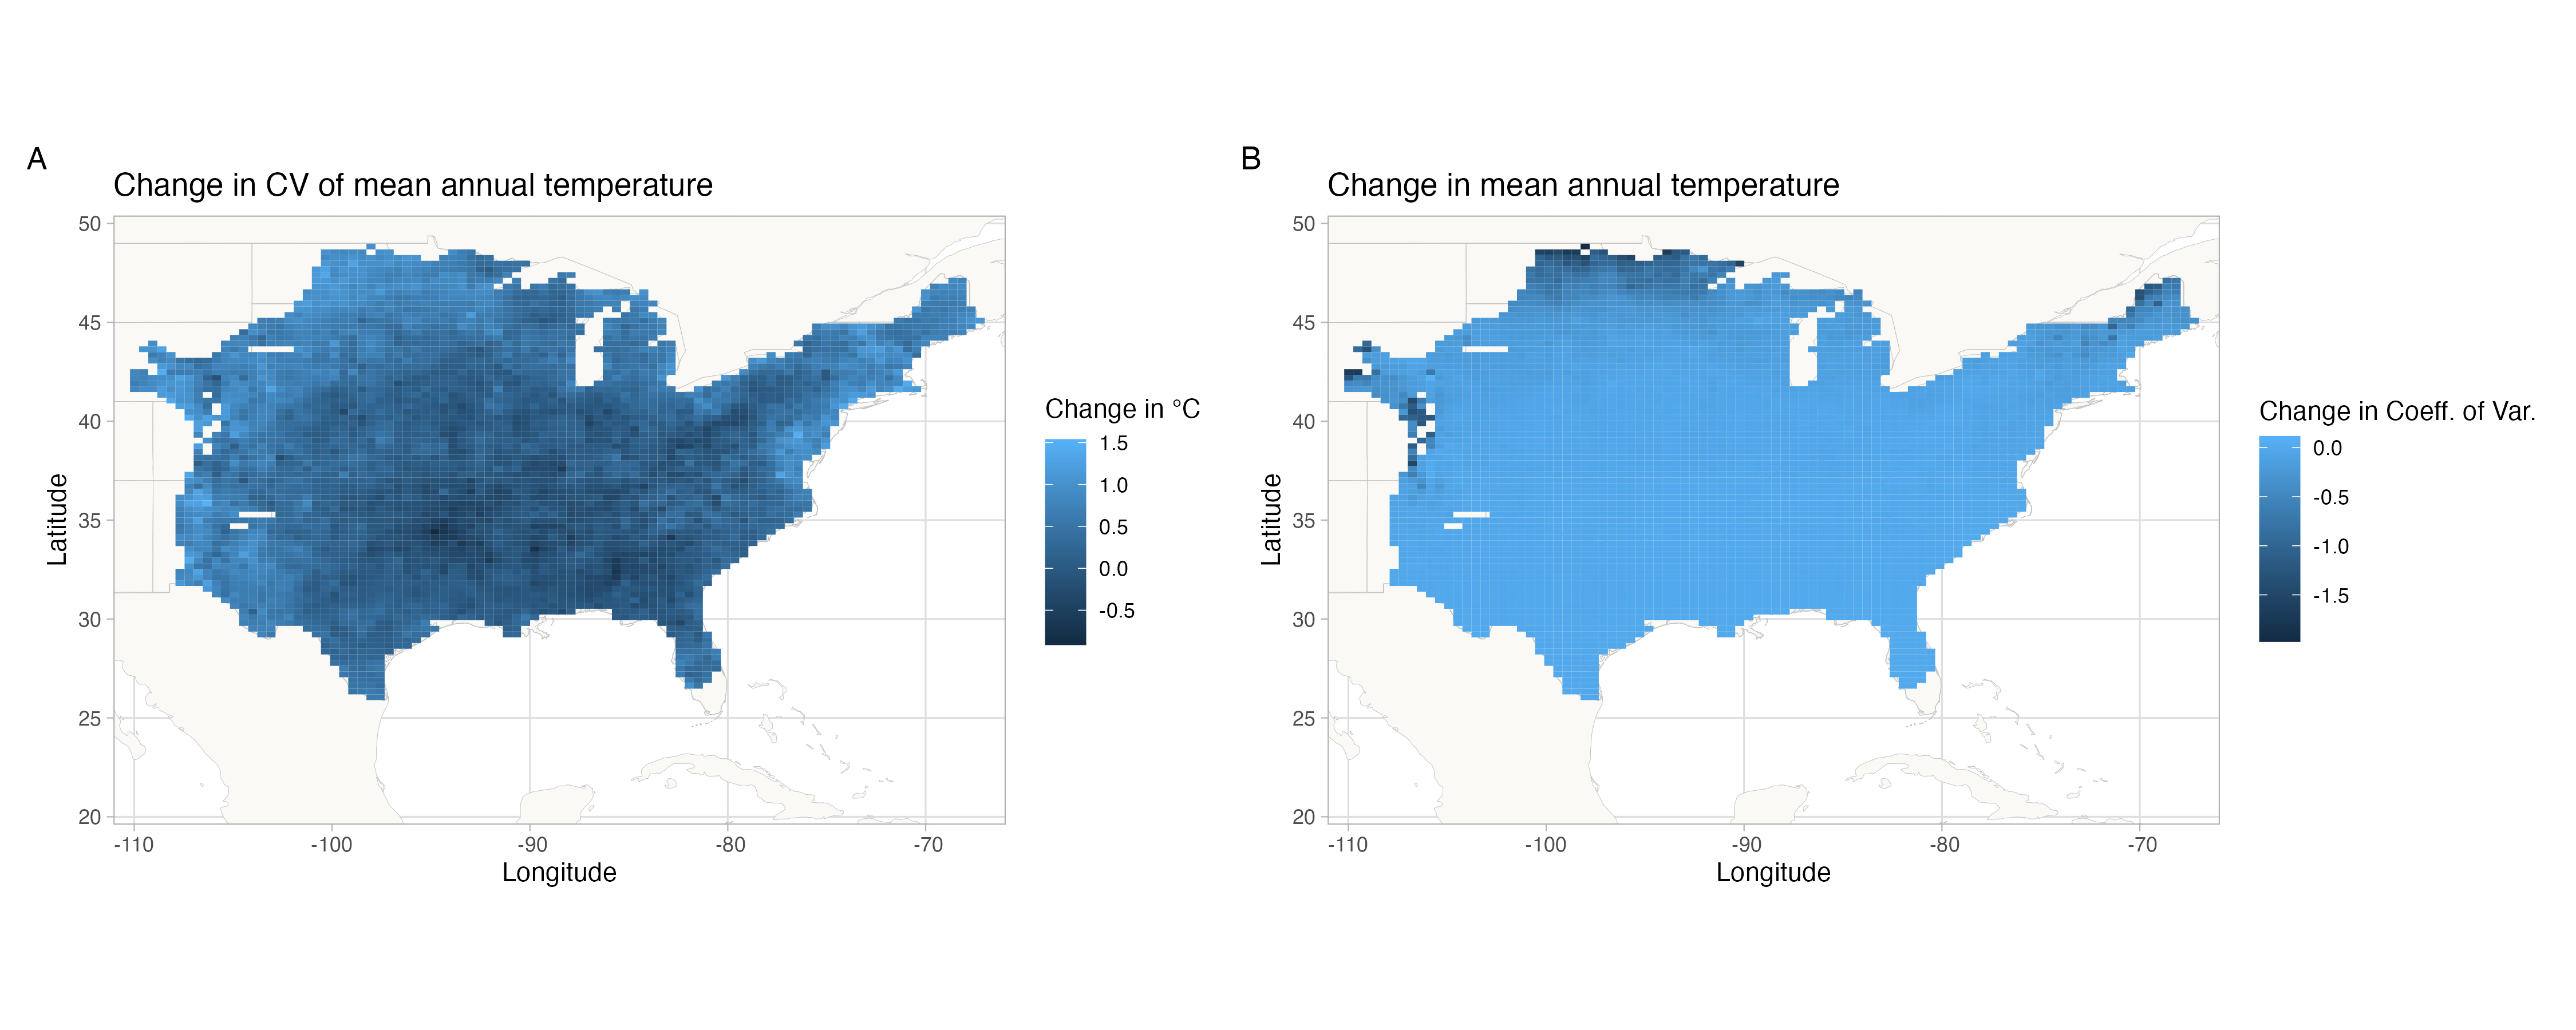
\includegraphics[width = \linewidth]{tmean_change_maps.png}
		\caption{\textbf{Change in temperature between the periods 1895-1925 and 1990-2020.} Color represents change in annual mean temperature (A) and in the coeffiecient of variation of annual mean temperature (B). Maps show the study area of \emph{A. hyemalis}. Map pixels used in correlation analysis with endophyte change were pulled from studies areas specific to each host species.}
	\end{figure}



\begin{figure}[H]
	\centering
	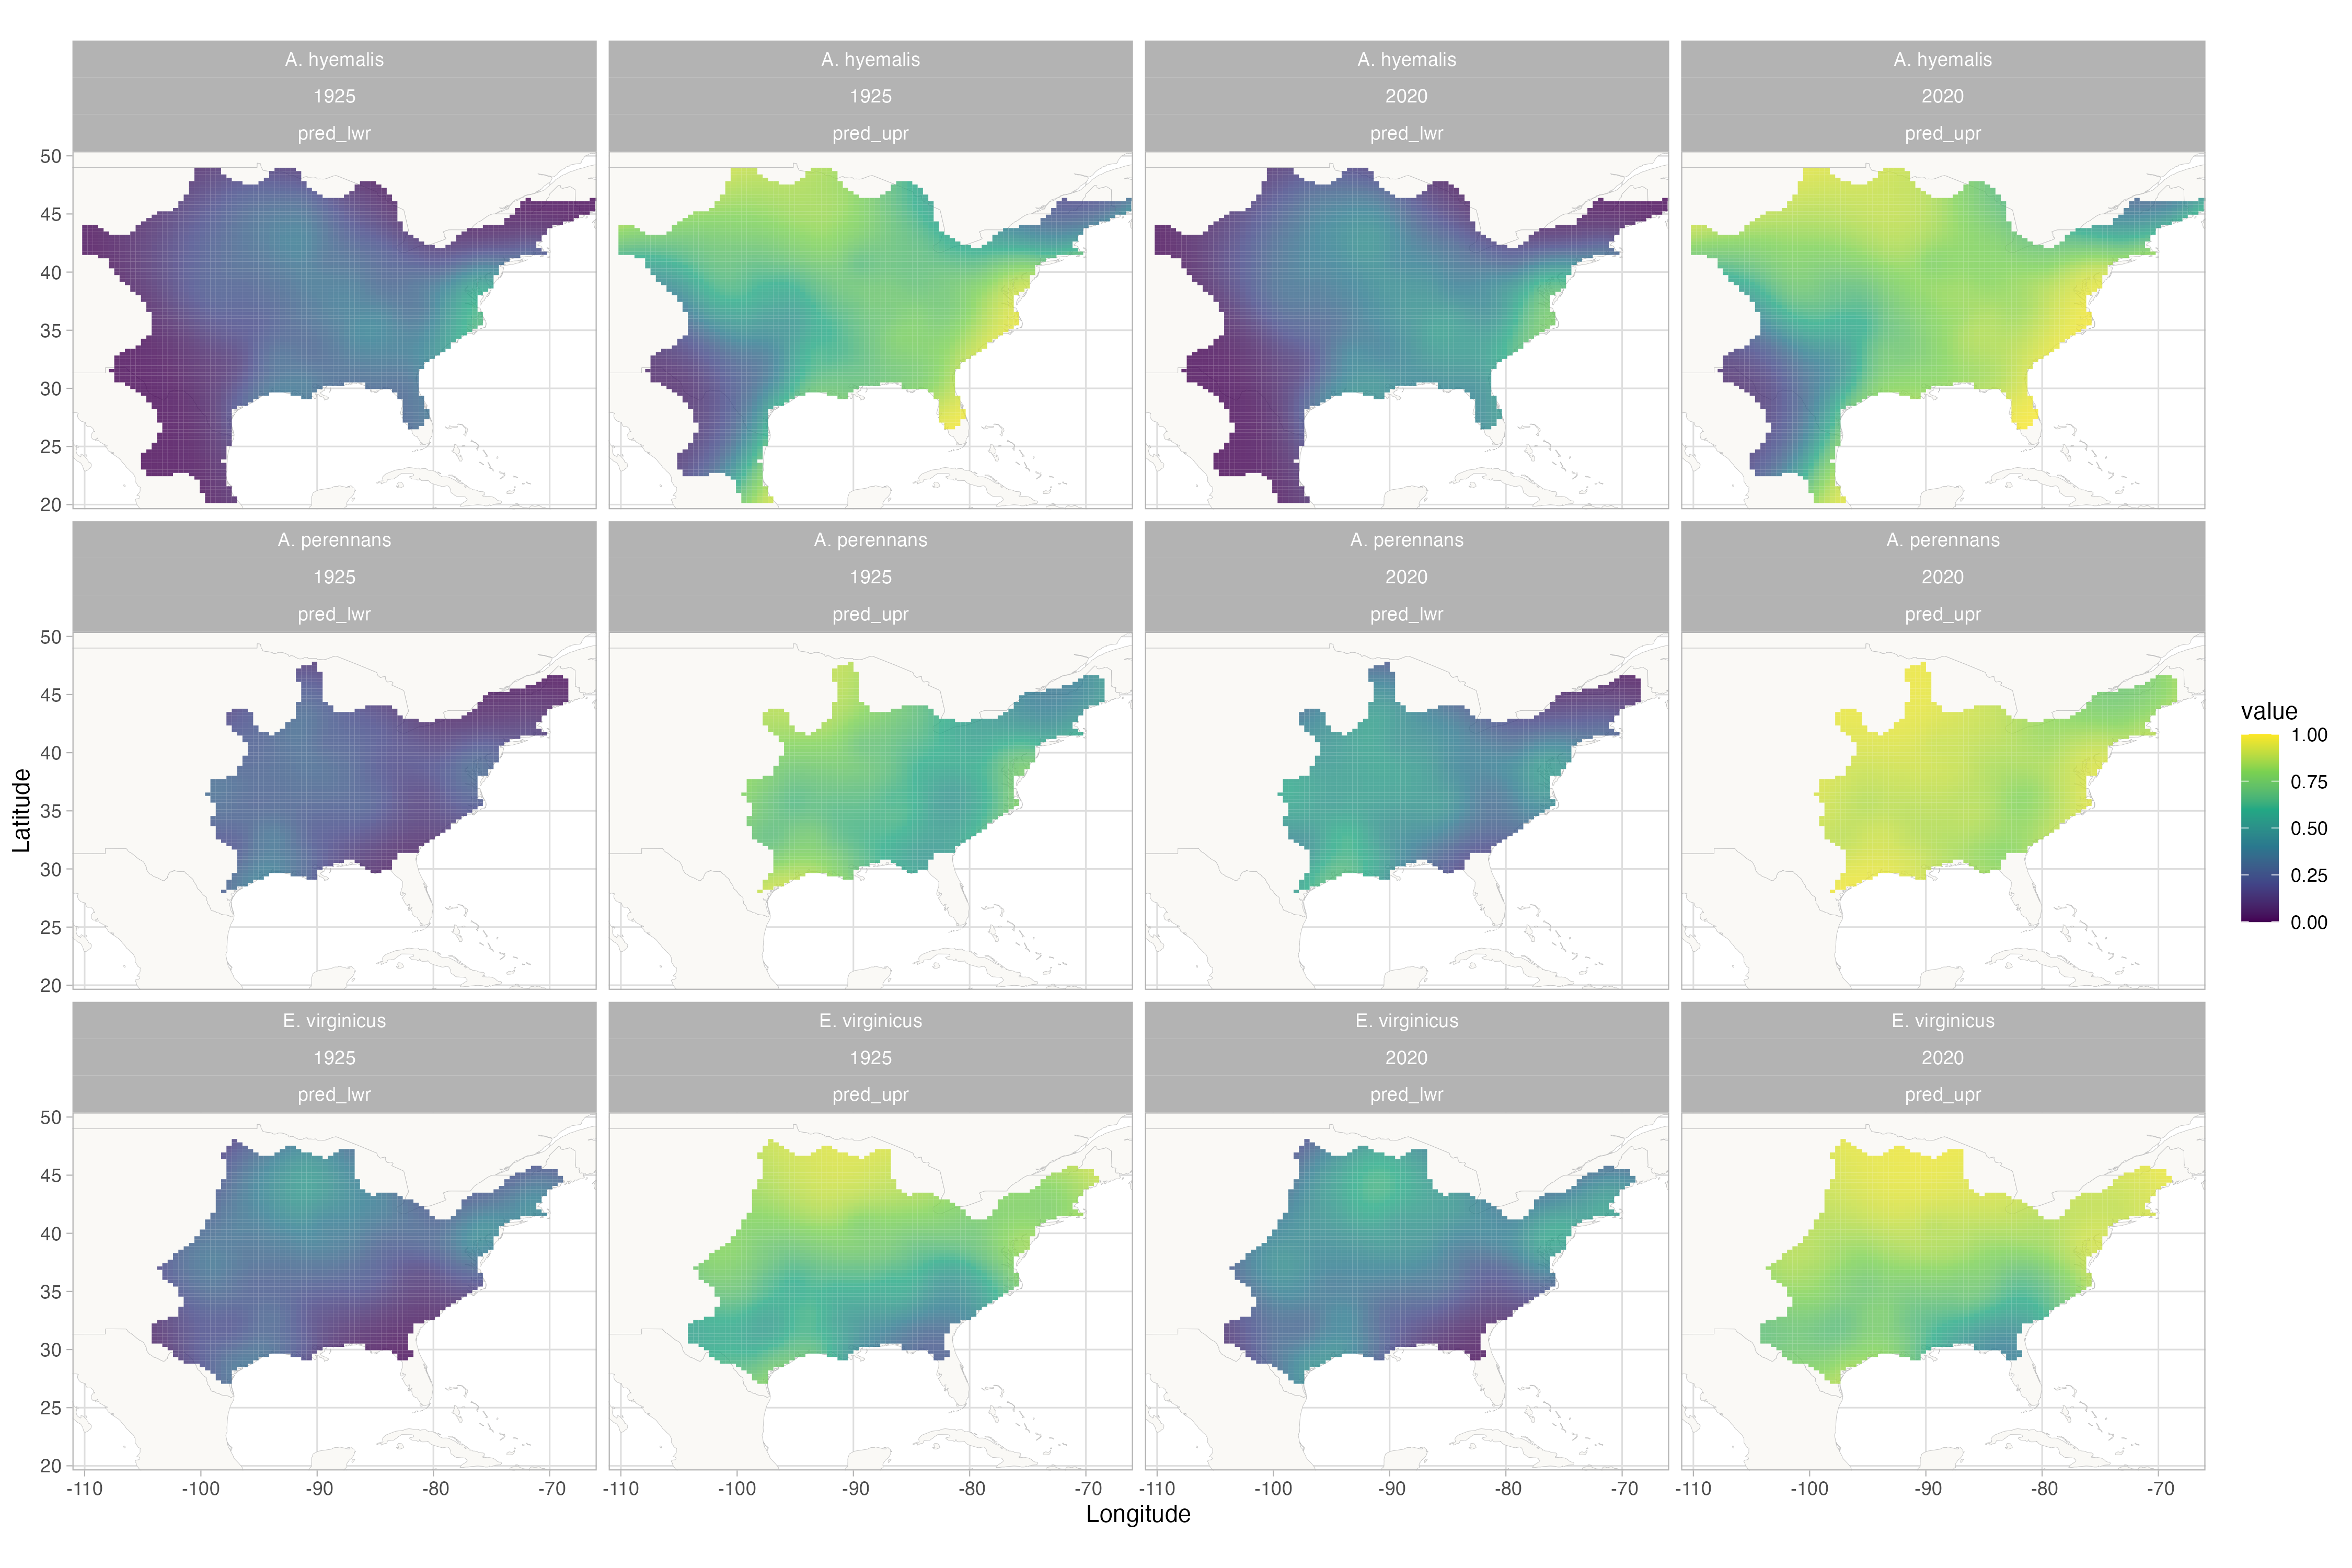
\includegraphics[width = \linewidth]{prevalence_map_CI.png}
	\caption{\textbf{Uncertainty associated with spatial trends in endophyte prevalence.} Color represents change in predicted endophyte prevalence. Panels show upper and lower 95\% posterior probability for each host species between 1925 and 2020.}
\end{figure}


\begin{figure}[H]
	\centering
	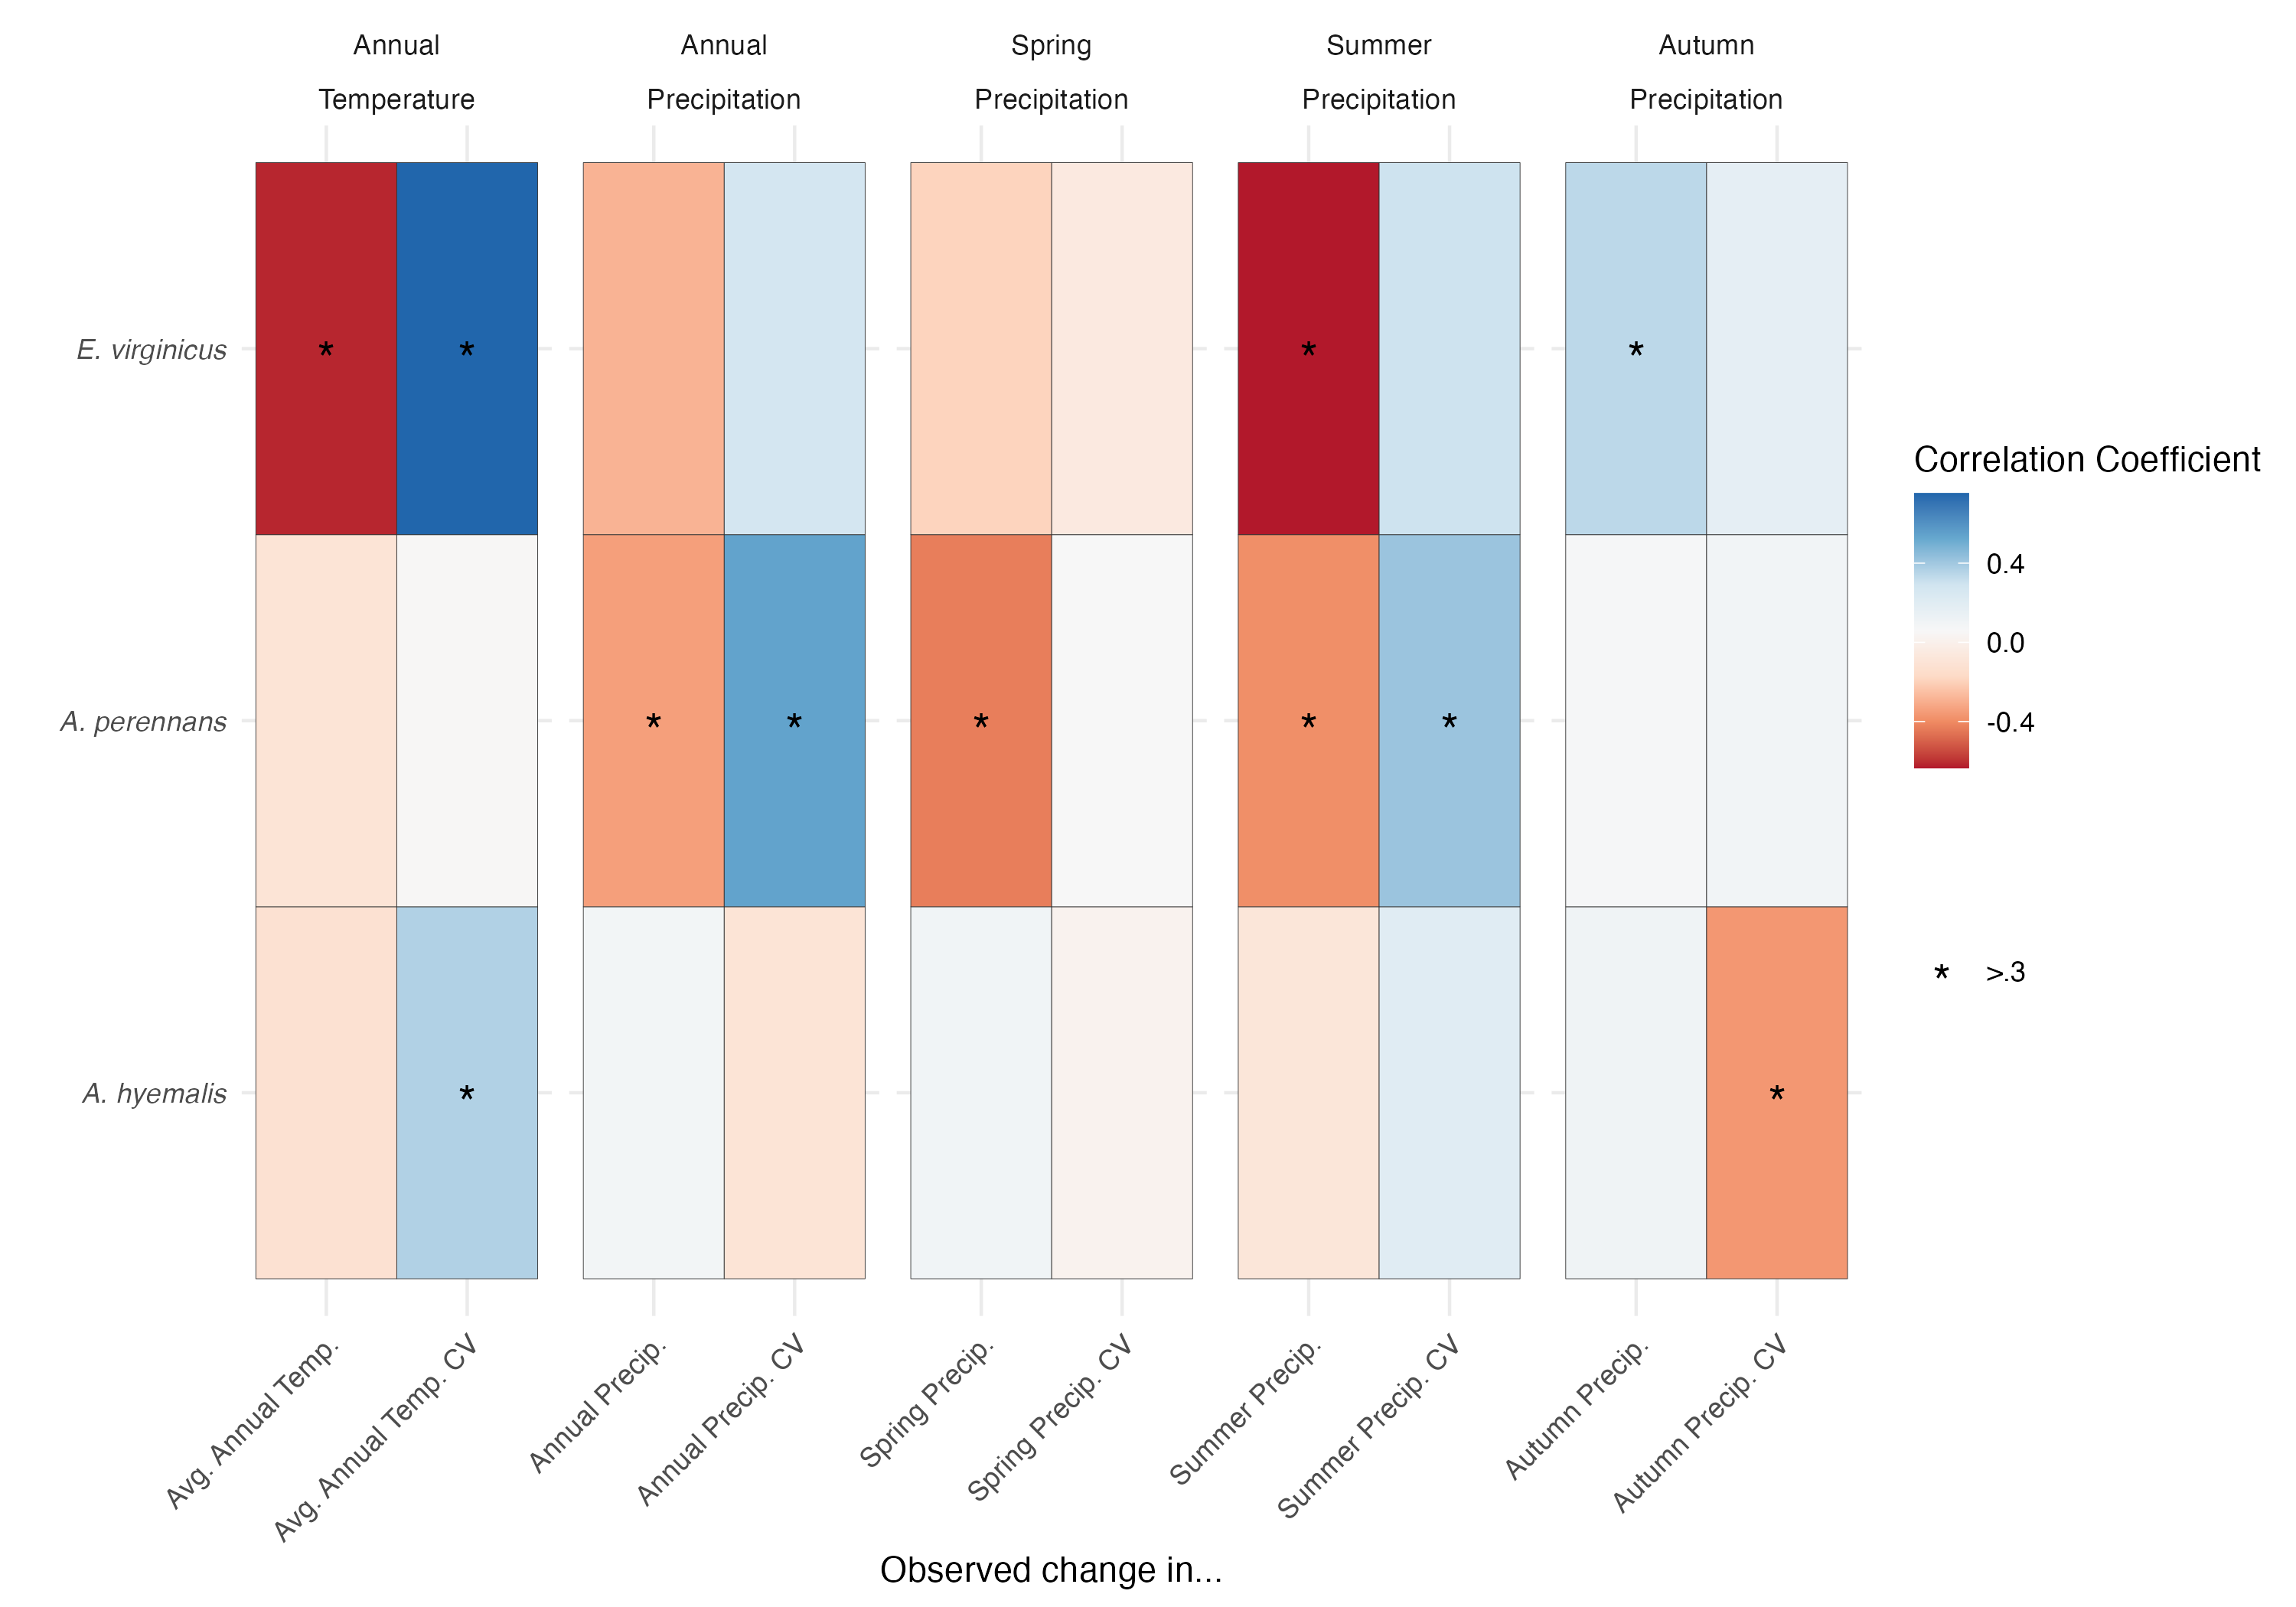
\includegraphics[width = \linewidth]{climate_corr_heatmap_subsample.png}
	\caption{\textbf{Correlations between changes in climate drivers and changes in endophyte prevalence from a random sample of 100 pixels across the study region.} Color denotes the Spearman correlation coefficient between the relative rate of change in endophyte prevalence and the change in annual mean temperature ($^oC$) and total annual and seasonal precipitation (mm), as well as the change in the coefficient of variation of each climate driver. Positive correlation coefficients indicate that greater increases in a climate driver were associated with larger increases in endophyte prevalence, while negative values indicate that . Asteriks denote correlation coefficients $> .3$ or $< -.3$.}
\end{figure}


	
	\begin{table}[h]
		\caption{Summary of herbarium samples across collections}
		\label{Table:herbaria}
		\centering
		\begin{tabular}{llll}\hline
			Herbarium Collection        & AGHY        & AGPE      &      ELVI\\ \hline
			Botanical Research Institute of Texas &   341   &    189&    176    \\
			Louisiana State University &     71  & --  &   61       \\
			Mercer Botanic Garden &   3    & --     &     6\\
			Missouri Botanic Garden& 78 & 39& 31\\
		    Texas A\&M &  73&-- & 49 \\
		    University of Kansas & 134 & -- &  20\\
		    University of Oklahoma & 65 &30&  91\\
		    University of Texas  \& Lundell   &  169& 41& 99\\		    				 			     			     
			Oklahoma State University&     30  &   --    &  69 \\ \hline
		\end{tabular}
		\bigskip{}

	\end{table}
	
	
	
	
	% In most cases, authors should typeset supplementary material in a separate,
	% author-supplied PDF. For author-supplied PDFs, please consult the
	% AmNat_supp_template.tex document, available from
	% https://www.journals.uchicago.edu/journals/an/instruct 
	%
	% By contrast, the Appendix instructions below apply to cases in which
	% a brief appendix is to appear in print after the main body of the article.
	% That notably includes descriptions of methods, tables defining parameters,
	% and other material necessary for reproducing the MS's results.
	%
	% Please reset counters for the appendix (thus normally figure A1, 
	% figure A2, table A1, etc.).
	%
	% Most AmNat articles have no more than one print appendix. If your article
	% has more than one, counters for each appendix should match the letter of
	% that appendix. For example, tables in Appendix B should be numbered table B1, % table C2, etc. This applies to tables, equations, and figures.
	%
	% It's better not to use the \appendix command, because we have some
	% formatting peculiarities that \appendix conflicts with.
	
	%%%%%%%%%%%%%%%%%%%%%
	% Bibliography
	%%%%%%%%%%%%%%%%%%%%%
	% You can either type your references following the examples below, or
	% compile your BiBTeX database and paste the contents of your .bbl file
	% here. The amnatnat.bst style file should work for this---but please
	% let us know if you run into any hitches with it!
	%
	% If you upload a .bib file with your submission, please upload the .bbl
	% file as well; this will be required for typesetting.
	%
	% The list below includes sample journal articles, book chapters, and
	% Dryad references.
	\newpage{}
\bibliographystyle{plainnat}
\bibliography{endo_herbarium}
	
	\newpage{}
	

	
\end{document}

